\documentclass[12pt,a4paper,bibliography=totocnumbered,listof=totocnumbered]{article}

% u.U. muss Koma-Skript Package ueber MikTeX deinstalliert und neu installiert werden
% Hilft das nicht, so sollte statt scrartcl die Dokumentenklasse article verwendet werden
\usepackage[backend=bibtex,style=alphabetic, natbib=true]{biblatex}
\usepackage[ngerman]{babel}
\usepackage[utf8]{inputenc}
\usepackage{ifthen}
\usepackage{xargs}
\usepackage{amsmath}
\usepackage{amsfonts}
\usepackage{amssymb}
\usepackage{graphicx}
\usepackage{fancyhdr}
\usepackage{tabularx}
\usepackage{geometry}
\usepackage{setspace}
\usepackage[right]{eurosym}
\usepackage[printonlyused]{acronym}
\usepackage{floatflt}
\usepackage[usenames,dvipsnames]{color}
\usepackage{colortbl}
\usepackage{paralist}
\usepackage{array}
\usepackage{titlesec}
\usepackage{parskip}
\usepackage[right]{eurosym}
\usepackage[titles]{tocloft}
\usepackage[pdfpagelabels=true]{hyperref}
%\usepackage[edges]{forest}
%\usepackage{caption}
\usepackage{subcaption}
\usepackage{booktabs}
\usepackage{mathtools} 
\usepackage{tikz}
\usepackage{tikz-qtree}
\usepackage{tikz-qtree-compat}
\usetikzlibrary{positioning}
\usepackage{forest}
\usepackage{filecontents}
%\usepackage[simplified]{pgf-umlcd}
\usepackage{tikz-uml}

\usetikzlibrary{arrows,matrix,positioning}
\usepackage{pgfplots}
\usetikzlibrary{calc}

\usepackage{wasysym}
\usepackage[automake]{glossaries-extra}
\usepackage{color}
\usepackage{listings}
\usepackage{longtable}
\lstset{basicstyle=\footnotesize, captionpos=b, breaklines=true, showstringspaces=false, tabsize=2, frame=lines, numbers=left, numberstyle=\tiny, xleftmargin=2em, framexleftmargin=2em}
\makeatletter
\def\l@lstlisting#1#2{\@dottedtocline{1}{0em}{1em}{\hspace{1,5em} Lst. #1}{#2}}
\makeatother

\geometry{a4paper, top=27mm, left=20mm, right=20mm, bottom=35mm, headsep=10mm, footskip=12mm}

\definecolor{javared}{rgb}{0.6,0,0} % for strings
\definecolor{javagreen}{rgb}{0.25,0.5,0.35} % comments
\definecolor{javapurple}{rgb}{0.5,0,0.35} % keywords
\definecolor{javadocblue}{rgb}{0.25,0.35,0.75} % javadoc
\definecolor{gray}{rgb}{0.6,0.6,0.6}
 
\lstset{language=Java,
basicstyle=\ttfamily\footnotesize,
keywordstyle=\color{javapurple}\bfseries,
stringstyle=\color{javared},
commentstyle=\color{javagreen}\itshape\bfseries,
morecomment=[s][\color{javadocblue}]{/**}{*/},
numbers=left,
numberstyle=\tiny\color{gray},
stepnumber=1,
numbersep=10pt,
tabsize=3,
showspaces=false,
showstringspaces=false}
% Kopf- und Fusszeile
\renewcommand{\sectionmark}[1]{\markright{#1}}
\renewcommand{\leftmark}{\rightmark}
\pagestyle{fancy}
\lhead{}
\chead{}
\rhead{\thesection\space\contentsname}
\lfoot{}
\cfoot{}
\rfoot{\ \linebreak Seite \thepage}
\renewcommand{\headrulewidth}{0.4pt}
\renewcommand{\footrulewidth}{0.4pt}

% Vorspann
\renewcommand{\thesection}{\Roman{section}}
\renewcommand{\theHsection}{\Roman{section}}
\pagenumbering{Roman}

\newcommand{\folgen}[1]{
\ensuremath
#1
}

\newcommandx{\student}[3][]{
	\def\studentName{#1}%
	\def\studentMatnr{#2}%
	\def\studentStudiengang{#3}%
}

\newcommandx{\MyTitelseite}[8][]{
\thispagestyle{empty}

\includegraphics[scale=0.2]{pics/oth-logo.png}%\hfill\includegraphics[scale=0.5]{#1}
\begin{center}
\ifthenelse{\equal{#2}{2}}{ % then
	\vspace*{2cm}
	\Large
	\textbf{Ostbayerische Technische Hochschule Regensburg}\\
	\textbf{Fakultät für Informatik und Mathematik}\\
	\vspace*{2cm}
	\Huge
	\textbf{#3}\\[1em]
	\large
	Zur Erlangung des akademischen Grades des\\
	\ifthenelse{\equal{#3}{Bachelorarbeit}}{Bachelor of Science (B.Sc.)}{Master of Science (M.Sc.)}\\
	\vspace*{1cm}
	\Large
	\textbf{#4}\\
}{ % else
	\vspace*{1cm}
	\Large
	\textbf{#4}\\
	\vspace*{2cm}
	\large
	An der Fakultät für Informatik und Mathematik der\\
	Ostbayerischen Technischen Hochschule Regensburg\\
	im Studiengang\\
	\studentStudiengang\\[2em]
	eingereichte\\
	\vspace*{1cm}
	\Large
	\textbf{#3}\\[2em]
	\large
	zur Erlangung des akademischen Grades des\\
	\ifthenelse{\equal{#3}{Bachelorarbeit}}{Bachelor of Science (B.Sc.)}{Master of Science (M.Sc.)}
	\vspace*{1cm}
	\Large
}
	\vfill
	\normalsize
	%\newcolumntype{x}[1]{>{\raggedleft\arraybackslash\hspace{0pt}}p{#1}}
	\begin{tabular}{rl}%{6cm}p{7.5cm}}
	    \rule{0mm}{1ex}\textbf{Vorgelegt von:} & \studentName \\
		\rule{0mm}{1ex}\textbf{Matrikelnummer:} & \hspace*{-0.5em}\begin{tabular}[t]{r}\studentMatnr\end{tabular} \\ 
		\ifthenelse{\equal{#2}{1}}{~\\}{\rule{0mm}{1ex}\textbf{Studiengang:} & \studentStudiengang \\[2em]}
		\rule{0mm}{1ex}\textbf{Erstgutachter:} & #5 \\ 
		\rule{0mm}{1ex}\textbf{Zweitgutachter:} & #6 \\[2em]
		\rule{0mm}{1ex}\textbf{Abgabedatum:} & #7 \\ 
	\end{tabular} 
\end{center}
\pagebreak
}
\addbibresource{literatur.bib}

\DefineBibliographyStrings{ngerman}{ 
	andothers = {{et\,al\adddot}},             
}
%\bibliographystyle{alpha}
\setstretch{1.15}
\newcommand{\tikzcircle}[2][red,fill=red]{\tikz[baseline=-0.5ex]\draw[#1,radius=#2] (0,0) circle ;}%

\newglossaryentry{alpha}
	{name=alpha,
	description={Bester Zug des Spielers}}

\makeglossaries

\newcolumntype{P}[1]{>{\centering\arraybackslash}p{#1}}


\begin{document}

% ----------------------------------------------------------------------------------------------------------
% Titelseite
% ----------------------------------------------------------------------------------------------------------
\newcommand{\studierenderName}{Josef Lanzl}
\student{\studierenderName}		% Studierender
{3170605}						% Matrikelnummer
{Medizinische Informatik}			% Studiengang

\MyTitelseite
{}	% Optionales Logo des extern betreuenden Unternehmens
{2}								% Style der Titelseite (1 oder 2)
{Bachelorarbeit}				% Typ der Abschlussarbeit (\in {Bachelorarbeit, Masterarbeit})
{Implementierung und Vergleich von Algorithmen basierend auf Monte-Carlo-Tree-Search und AlphaZero für das strategische Brettspiel Reversi}				% Thema der Arbeit						
{Prof.\ Dr.\ Carsten Kern}		% Betreuer
{Prof.\ Dr.\ Christoph Palm}	% Zweitgutachter
{28.02.\the\year}				% Abgabedatum

\thispagestyle{empty}
~\pagebreak

\setcounter{page}{1} 

% ----------------------------------------------------------------------------------------------------------
% Eigenständigkeitserklaerung
% ----------------------------------------------------------------------------------------------------------
\thispagestyle{empty}
\section*{Erklärung zur Bachelorarbeit}

\bigskip
\bigskip 
\bigskip 

\begin{enumerate}
    \item Mir ist bekannt, dass dieses Exemplar der Abschlussarbeit als Prüfungsleistung in das Eigentum der Ostbayerischen Technischen Hochschule Regensburg übergeht.
    \item Ich erkläre hiermit, dass ich diese Abschlussarbeit selbständig verfasst, noch nicht anderweitig für Prüfungszwecke vorgelegt, keine anderen als die angegebenen Quellen und Hilfsmittel benutzt sowie wörtliche und sinngemäße Zitate als solche gekennzeichnet habe.
\end{enumerate}

\bigskip 
\bigskip 
\bigskip 

Regensburg, den \today

\bigskip 
\bigskip

\line(1,0){200}
\newline
\studierenderName

% ----------------------------------------------------------------------------------------------------------
% Abstract
% ----------------------------------------------------------------------------------------------------------
\thispagestyle{empty}
\setstretch{1.15} % Zeilenspacing
\section*{Zusammenfassung}

\bigskip 


In der vorliegenden Bachelorarbeit werden Algorithmen basierend auf Monte-Carlo-Tree-Search und AlphaZero verglichen. Die Algorithmen werden auf das Brettspiel Reversi angewendet. Das Ziel dieser Arbeit ist die Überprüfung einer Verbesserung dieser Kombinationen, bestehend aus konventioneller Implementierung und maschinellen Lernen, gegenüber dem klassischen Monte-Carlo-Tree-Search. Es werden vier Hybrid-Algorithmen, bestehend aus Kombinationen von Monte-Carlo-Tree-Search und MiniMax, ausgewertet und ihre Leistung anhand ausgewählter Parameter verglichen.\\
Anschließend wird AlphaZero, eine Kombination aus einem neuronalen Netz und Monte-Carlo-Tree-Search, vorgestellt, ebenfalls auf Reversi angewendet und dessen Ergebnisse ausgewertet.\\
Die Umsetzung und Implementierung dieser Algorithmen wird hinzukommend beschrieben.\\
Es konnte gezeigt werden, dass die Kombinationen mit MiniMax an verschiedenen Stellen des Algorithmus nicht zu auffallenden Verbesserungen beigetragen haben. Die Siegesraten waren nicht besser wie die des Basisalgorithmus Monte-Carlo-Tree-Search.\\
Die Umsetzung des Lernens des Spiels Reversi mit einem residualen Netz konnte umgesetzt werden. Dessen Auswertung führte bei einer trivialen KI als Gegner zu einer Siegesraten von über 70\%. Das Ergebnis wird abschließend anhand eines Vergleichs mit aus der Literatur bekannten neuronalen Netzen, welche Faltungsnetze verwenden, verglichen und eingeordnet.

\section*{Abstract}

\bigskip 


In this bachelor thesis, algorithms based on Monte-Carlo-Tree-Search and AlphaZero are compared. The algorithms are applied to the board game Reversi. The goal of this work is to verify an improvement of these combinations, consisting of conventional implementation and machine learning, over classical Monte-Carlo Tree Search. Four hybrid algorithms, consisting of combinations of Monte-Carlo Tree Search and MiniMax, are evaluated and their performance is compared based on selected parameters.\\
AlphaZero, a combination of a neural network and Monte-Carlo Tree Search, is then presented, also applied to Reversi, and its results evaluated.\\
The realization and implementation of these algorithms is described in addition.\\
It was shown that the combinations with MiniMax at different points of the algorithm did not contribute to striking improvements. The win rates were not better than those of the basic Monte Carlo Tree Search algorithm.\\
The implementation of learning the game Reversi with a residual network could be implemented. Its evaluation led to a win rate of over 70\% with a trivial AI as opponent. Finally, the result is compared and classified with neural networks known from the literature, which use convolutional networks.


% ----------------------------------------------------------------------------------------------------------
% Inhaltsverzeichnis
% ----------------------------------------------------------------------------------------------------------
\tableofcontents
\pagebreak

% ----------------------------------------------------------------------------------------------------------
% Abbildungsverzeichnis
% ----------------------------------------------------------------------------------------------------------
\lhead{}
\rhead{Abbildungsverzeichnis}
\listoffigures
\pagebreak

% ----------------------------------------------------------------------------------------------------------
% Tabellenverzeichnis (optional)
% ----------------------------------------------------------------------------------------------------------
\lhead{}
\rhead{Tabellenverzeichnis}
\listoftables



% ----------------------------------------------------------------------------------------------------------
% Listingsverzeichnis (optional; Code nur, wenn wirklich sinnvoll und wichtig)
% ----------------------------------------------------------------------------------------------------------
%\lhead{}
%\rhead{Quellcodeverzeichnis}
%\lstlistoflistings
%\pagebreak

% ----------------------------------------------------------------------------------------------------------
% Abkürzungsverzeichnis (optional)
% ----------------------------------------------------------------------------------------------------------
\lhead{}
\rhead{Abkürzungsverzeichnis}
%\listoftables
\section{Abkürzungsverzeichnis}
\begin{longtable}{p{3.5 cm}p{12 cm}} 
  KI & Künstliche Intelligenz \\
  MCTS & Monte-Carlo-Tree-Search \\
  MCTS-IPM & Monte-Carlo-Tree-Search mit Informed Priors und MiniMax\\
  MCTS-MB & Monte-Carlo-Tree-Search mit MiniMax in Backpropagation\\
  MCTS-MR & Monte-Carlo-Tree-Search mit MiniMax im Rollout\\
  MCTS-MS & Monte-Carlo-Tree-Search mit MiniMax in Selektion und Expansion\\
  ReLU & Rectified-Linear-Unit Funktion\\
  TaM & Tatsächliche Mobilität\\
  UCT & Upper-Confidence-Bound-for-Trees-Strategie\\
\end{longtable}
\setcounter{table}{0}
\pagebreak


% ----------------------------------------------------------------------------------------------------------
% Inhalt
% ----------------------------------------------------------------------------------------------------------
% Abstände Überschrift
\titlespacing{\section}{0pt}{12pt plus 4pt minus 2pt}{8pt plus 2pt minus 2pt}
\titlespacing{\subsection}{0pt}{12pt plus 4pt minus 2pt}{6pt plus 2pt minus 2pt}
\titlespacing{\subsubsection}{0pt}{12pt plus 4pt minus 2pt}{4pt plus 2pt minus 2pt}

% Kopfzeile
\renewcommand{\sectionmark}[1]{\markright{#1}}
\renewcommand{\subsectionmark}[1]{}
\renewcommand{\subsubsectionmark}[1]{}
\lhead{Kapitel \thesection}
\rhead{\rightmark}

%\onehalfspacing
\setstretch{1.15}
\renewcommand{\thesection}{\arabic{section}}
\renewcommand{\theHsection}{\arabic{section}}
\setcounter{section}{0}
\pagenumbering{arabic}
\setcounter{page}{1}

% ----------------------------------------------------------------------------------
% Kapitel: Einleitung
% ----------------------------------------------------------------------------------
\section{Einleitung}
Das Themengebiet der künstlichen Intelligenz hat in den vergangenen Jahren immer mehr an Relevanz gewonnen. Zu Brettspielen, die bereits von Algorithmen gelöst sind, zählen beispielsweise Mühle und Vier Gewinnt. Das Spiel Othello konnte bisher nur auf einem 6x6 Spielfeld gelöst werden \cite{vandenHerik.2002}.\\
Der auf künstlicher Intelligenz basierende Algorithmus AlphaZero ist ein verallgemeinerter Ansatz von AlphaGo Zero, dessen Ergebnisse bereits menschliches Können im Spiel Go übertrifft und professionelle Spieler besiegt hat. AlphaZero ist ein Ansatz, der für weitere Brettspiele erweitert ist \cite{Silver.05.12.2017} und verwendet den Algorithmus Monte-Carlo-Tree-Search, welcher ohne Heuristiken Spielbäume anhand zufälliger Werte aufbaut und laut \cite{CameronBrowne.2012} bereits Erfolge im Spiel Go und in weiteren Einsatzgebieten erzielte. Aufgrund der Erfolge der vorher genannten Algorithmen, ist es interessant diese auf das Brettspiel Reversi anzuwenden.

%Baier und Winands haben aufgrund der Erfolge von Monte-Carlo-Tree-Search und MiniMax in \cite{Baier.2015} mehrere Ansätze zu Kombination dieser Algorithmen beschrieben und ausgewertet. Diese Ansätze verzichten auf den Einsatz von Heuristiken. In \cite{Baier.2018} sind weitere Möglichkeiten dieser Hybridalgorithmen unter Verwendung von Heuristiken dargelegt.
% ----------------------------------------------------------------------------------
% Kapitel: Motivation
% ----------------------------------------------------------------------------------
%Motivation dieser Arbeit ist der Vergleich der Ansätze künstlicher Intelligenz basierend auf konventioneller Implementierung und dem Verwenden eines neuronalen Netzes. Zusätzlich ist eine weitere Motivation dieser Arbeit das Überprüfen, ob die Kombination zweier bereits erfolgreicher Algorithmen tatsächlich einen noch besseren Algorithmus erschaffen.

Die Aufgabe dieser Arbeit soll es sein, Zusammenhänge zwischen Spielbaum-Algorithmen und neuronalen Netzen in Kombination mit dem Brettspiel Reversi besser verstehen zu können und das bestmögliche Ergebnis dieses Netzes zu erreichen. Eine weitere Motivation liegt in der Implementierung und Anwendung dieser Algorithmen. Des Weiteren wird der Hypothese nachgegangen, ob das Kombinieren zweier Algorithmen tatsächlich einen überlegeneren Algorithmus ergibt, welcher bezüglich der Anzahl an Siege bessere Ergebnisse liefert als seine Basis-Algorithmen.

Ein Ziel dieser Arbeit ist zum Einen das Überprüfen der Verbesserung der Hybrid-Algorithmen von Baier und Winands. Hierfür werden drei verschiedene Ansätze ohne Heuristik und einer mit der Verwendung einer Heuristik betrachtet. Ein weiteres Ziel ist das Überprüfen der resultierenden Leistungsverbesserung durch die Kombination von Monte-Carlo-Tree-Search und neuronalem Netz, in Form von AlphaZero.

Wie bereits beschrieben, basieren die Kombinationen aus MiniMax und Monte-Carlo-Tree-Search auf den Forschungsergebnissen von Baier und Winands \cite{Baier.2015} \cite{Baier.2018}. AlphaZero hingegen ist ein von DeepMind entworfener Ansatz zum Training eines neuronalen Netzes für Brettspiele, der in der Literatur durch \cite{Silver.05.12.2017} erstmal auf Brettspiele angewendet wurde. Der Einsatz eines neuronalen Netzes für das Lernen des Spiels Othello basierend auf AlphaGo Zero ist in \cite{Shantanu.2018} aufgegriffen. Ein weiterer Ansatz, welcher nicht auf AlphaZero basiert und trotzdem gute Ergebnisse mit einem Faltungsnetz erzielt hat, ist in \cite{Liskowski.2018} beschrieben.

Im Rahmen dieser Arbeit werden zunächst die grundlegenden Fragen geklärt, was unter künst-licher Intelligenz und insbesondere neuronalen Netzen zu verstehen ist. Des Weiteren werden die Algorithmen Monte-Carlo-Tree-Search, MiniMax und deren Kombinationen erläutert. Anschließend werden im praktischen Teil die Ergebnisse der Versuche der Hybrid-Algorithmen und des Trainings des neuronalen Netzes in Kombination mit dem Brettspiel Reversi dargelegt und diskutiert. Abschließend wird ein Fazit zu diesen Ergebnissen gezogen.


\pagebreak
% ----------------------------------------------------------------------------------
% Kapitel: Theorie
% ----------------------------------------------------------------------------------
\section{Grundlagen}
Ziel dieses Kapitels ist es, die Grundlagen zur Theorie für diese Arbeit zu vermitteln. Zu Beginn wird kurz auf das Brettspiel Reversi eingegangen. Anschließend werden Begriffe wie künstliche Intelligenz, maschinelles Lernen und insbesondere tiefes Lernen sowie neuronale Netze erläutert. Der nächste Abschnitt behandelt Heuristiken bezogen auf Reversi. Des Weiteren werden Bäume sowie Spielbäume thematisiert, da die Algorithmen MiniMax und Monte-Carlo-Tree-Search der Folgekapitel darauf basieren. Abschließend wird der von DeepMind veröffentliche AlphaZero-Ansatz verdeutlicht.

% ----------------------------------------------------------------------------------
% Kapitel: Reversi
% ----------------------------------------------------------------------------------
\subsection{Reversi}
Reversi, auch bekannt als Othello \cite[S. 31]{Russell.2012}, ist ein rundenbasiertes Strategiebrettspiel, bei dem zwei Spieler gegeneinander antreten. Das Spiel wird auf einem quadratischen Brett mit 64 Feldern und unterscheidbaren Figuren gespielt. Im Startzustand befinden sich die Spielsteine immer in der Mitte (siehe \autoref{abb:reversi-start}). Im Folgenden werden die Koordinaten des Spielfelds als $(x, y)$ bezeichnet, wobei gilt $x,y \in [1,8]$. Der Parameter $x$ beschreibt hierbei die Position in der Spielfeldbreite, $y$ die Position in der Spielfeldhöhe. Ein Zug $z$ nach Punkt $p \in (x, y)$ wird mit $z(p)$ abgekürzt. \\
Ist ein Spieler am Zug, muss dieser, ausgehend von einem eigenen Stein, mindestens einen gegnerischen Spielstein überspringen und anschließend auf einem freien Zielfeld landen. Das freie Zielfeld und alle eingeschlossenen Steine des Gegners werden von den eigenen Spielsteinen belegt. Werden Steine des Kontrahenten auch aus anderen Richtungen eingeschlossen, so werden auch diese durch eigene Steine ersetzt. Ein Beispielzug wird in \autoref{abb:reversi-zug} dargestellt. Hier zieht Spieler A, welcher mit den schwarzen Figuren spielt, nach Position $(5,3)$.

\begin{figure} [h]
\centering
\begin{minipage}[b]{0.45\textwidth}
\centering
   \begin{tabular}{m{0.2cm}m{0.2cm}m{0.2cm}m{0.2cm}m{0.2cm}m{0.2cm}m{0.2cm}m{0.2cm}m{0.2cm}}
                       & 1                     & 2                     & 3                                             & 4                                             & 5                                             & 6                                             & 7                     & 8                     \\ \cline{2-9} 
\multicolumn{1}{l|}{1} & \multicolumn{1}{l|}{} & \multicolumn{1}{l|}{} & \multicolumn{1}{l|}{}                         & \multicolumn{1}{l|}{}                         & \multicolumn{1}{l|}{}                         & \multicolumn{1}{l|}{}                         & \multicolumn{1}{l|}{} & \multicolumn{1}{l|}{} \\ \cline{2-9} 
\multicolumn{1}{l|}{2} & \multicolumn{1}{l|}{} & \multicolumn{1}{l|}{} & \multicolumn{1}{l|}{}                         & \multicolumn{1}{l|}{}                         & \multicolumn{1}{l|}{}                         & \multicolumn{1}{l|}{}                         & \multicolumn{1}{l|}{} & \multicolumn{1}{l|}{} \\ \cline{2-9} 
\multicolumn{1}{l|}{3} & \multicolumn{1}{l|}{} & \multicolumn{1}{l|}{} & \multicolumn{1}{l|}{}                         & \multicolumn{1}{l|}{}                         & \multicolumn{1}{l|}{\cellcolor{yellow}} & \multicolumn{1}{l|}{}                         & \multicolumn{1}{l|}{} & \multicolumn{1}{l|}{} \\ \cline{2-9} 
\multicolumn{1}{l|}{4} & \multicolumn{1}{l|}{} & \multicolumn{1}{l|}{} & \multicolumn{1}{l|}{}                         & \multicolumn{1}{l|}{ \tikzcircle[fill=black]{3pt} }                        & \multicolumn{1}{l|}{\tikzcircle[fill=white]{3pt}}                        & \multicolumn{1}{l|}{\cellcolor{yellow}} & \multicolumn{1}{l|}{} & \multicolumn{1}{l|}{} \\ \cline{2-9} 
\multicolumn{1}{l|}{5} & \multicolumn{1}{l|}{} & \multicolumn{1}{l|}{} & \multicolumn{1}{l|}{\cellcolor{yellow}} & \multicolumn{1}{l|}{\tikzcircle[fill=white]{3pt}}                        & \multicolumn{1}{l|}{ \tikzcircle[fill=black]{3pt} }                        & \multicolumn{1}{l|}{}                         & \multicolumn{1}{l|}{} & \multicolumn{1}{l|}{} \\ \cline{2-9} 
\multicolumn{1}{l|}{6} & \multicolumn{1}{l|}{} & \multicolumn{1}{l|}{} & \multicolumn{1}{l|}{}                         & \multicolumn{1}{l|}{\cellcolor{yellow}} & \multicolumn{1}{l|}{}                         & \multicolumn{1}{l|}{}                         & \multicolumn{1}{l|}{} & \multicolumn{1}{l|}{} \\ \cline{2-9} 
\multicolumn{1}{l|}{7} & \multicolumn{1}{l|}{} & \multicolumn{1}{l|}{} & \multicolumn{1}{l|}{}                         & \multicolumn{1}{l|}{}                         & \multicolumn{1}{l|}{}                         & \multicolumn{1}{l|}{}                         & \multicolumn{1}{l|}{} & \multicolumn{1}{l|}{} \\ \cline{2-9} 
\multicolumn{1}{l|}{8} & \multicolumn{1}{l|}{} & \multicolumn{1}{l|}{} & \multicolumn{1}{l|}{}                         & \multicolumn{1}{l|}{}                         & \multicolumn{1}{l|}{}                         & \multicolumn{1}{l|}{}                         & \multicolumn{1}{l|}{} & \multicolumn{1}{l|}{} \\ \cline{2-9} 
\end{tabular}
    \subcaption{Startzustand des Spiels}
    \label{abb:reversi-start}

\end{minipage}
\qquad
\begin{minipage}[b]{0.45\textwidth}
\centering
   \begin{tabular}{m{0.2cm}m{0.2cm}m{0.2cm}m{0.2cm}m{0.2cm}m{0.2cm}m{0.2cm}m{0.2cm}m{0.2cm}}
                       & 1                     & 2                     & 3                     & 4                                             & 5                      & 6                                             & 7                     & 8                     \\ \cline{2-9} 
\multicolumn{1}{l|}{1} & \multicolumn{1}{l|}{} & \multicolumn{1}{l|}{} & \multicolumn{1}{l|}{} & \multicolumn{1}{l|}{}                         & \multicolumn{1}{l|}{}  & \multicolumn{1}{l|}{}                         & \multicolumn{1}{l|}{} & \multicolumn{1}{l|}{} \\ \cline{2-9} 
\multicolumn{1}{l|}{2} & \multicolumn{1}{l|}{} & \multicolumn{1}{l|}{} & \multicolumn{1}{l|}{} & \multicolumn{1}{l|}{}                         & \multicolumn{1}{l|}{}  & \multicolumn{1}{l|}{}                         & \multicolumn{1}{l|}{} & \multicolumn{1}{l|}{} \\ \cline{2-9} 
\multicolumn{1}{l|}{3} & \multicolumn{1}{l|}{} & \multicolumn{1}{l|}{} & \multicolumn{1}{l|}{} & \multicolumn{1}{l|}{\cellcolor{yellow}} & \multicolumn{1}{l|}{\tikzcircle[fill=black]{3pt}} & \multicolumn{1}{l|}{\cellcolor{yellow}} & \multicolumn{1}{l|}{} & \multicolumn{1}{l|}{} \\ \cline{2-9} 
\multicolumn{1}{l|}{4} & \multicolumn{1}{l|}{} & \multicolumn{1}{l|}{} & \multicolumn{1}{l|}{} & \multicolumn{1}{l|}{\tikzcircle[fill=black]{3pt}}                        & \multicolumn{1}{l|}{\tikzcircle[fill=black]{3pt}} & \multicolumn{1}{l|}{}                         & \multicolumn{1}{l|}{} & \multicolumn{1}{l|}{} \\ \cline{2-9} 
\multicolumn{1}{l|}{5} & \multicolumn{1}{l|}{} & \multicolumn{1}{l|}{} & \multicolumn{1}{l|}{} & \multicolumn{1}{l|}{\tikzcircle[fill=white]{3pt}}                        & \multicolumn{1}{l|}{\tikzcircle[fill=black]{3pt}} & \multicolumn{1}{l|}{\cellcolor{yellow}} & \multicolumn{1}{l|}{} & \multicolumn{1}{l|}{} \\ \cline{2-9} 
\multicolumn{1}{l|}{6} & \multicolumn{1}{l|}{} & \multicolumn{1}{l|}{} & \multicolumn{1}{l|}{} & \multicolumn{1}{l|}{}                         & \multicolumn{1}{l|}{}  & \multicolumn{1}{l|}{}                         & \multicolumn{1}{l|}{} & \multicolumn{1}{l|}{} \\ \cline{2-9} 
\multicolumn{1}{l|}{7} & \multicolumn{1}{l|}{} & \multicolumn{1}{l|}{} & \multicolumn{1}{l|}{} & \multicolumn{1}{l|}{}                         & \multicolumn{1}{l|}{}  & \multicolumn{1}{l|}{}                         & \multicolumn{1}{l|}{} & \multicolumn{1}{l|}{} \\ \cline{2-9} 
\multicolumn{1}{l|}{8} & \multicolumn{1}{l|}{} & \multicolumn{1}{l|}{} & \multicolumn{1}{l|}{} & \multicolumn{1}{l|}{}                         & \multicolumn{1}{l|}{}  & \multicolumn{1}{l|}{}                         & \multicolumn{1}{l|}{} & \multicolumn{1}{l|}{} \\ \cline{2-9} 
\end{tabular}
    \subcaption{Schwarz zieht nach $(5,3)$}
    \label{abb:reversi-zug}

\end{minipage}
\caption{Spielzustände in Reversi}

\label{abb:reversi}
\end{figure}

Die möglichen Züge, die Spieler B mit den weißen Figuren anschließend durchführen kann, sind hierbei markiert. Das Ende des Spiels ist erreicht, falls keiner der beiden Spieler einen weiteren Zug machen kann und der Teilnehmer mit den meist besetzten Feldern gewinnt \citep{NikLever.2012}. Wie nun eine künstliche Intelligenz ein Brettspiel lernen kann, wird im folgenden Kapitel erläutert.

% ----------------------------------------------------------------------------------
% Kapitel: Künstliche Intelligenz
% ----------------------------------------------------------------------------------
\subsection{Künstliche Intelligenz}
Das Ziel einer \emph{künstlichen Intelligenz} (KI) ist es, den Menschen in seinen intellektuellen Fähig-keiten gleichauf zu sein oder diesen zu übertreffen \citep[S. 14]{Frochte.2019}.\\
Hierbei wird zwischen starker und schwacher KI unterschieden. Eine starke KI ist in vielen Einsatzgebieten dem Menschen mindestens gleichwertig, wohingegen die schwache KI nur auf einem Gebiet spezialisiert ist. Diese Gebiete umfassen das Lösen komplexer Aufgaben, wie beispielsweise der Bilderkennung oder dem Spielen von komplexen Brettspielen. Beide Arten der KI können in ihren Leistungen den Menschen übertreffen. Hierbei ist jedoch anzumerken, dass eine starke KI in der Praxis bisher noch nicht erreicht wurde \citep[S.21]{UweLammel.2020}. Das Ziel einer KI in der Informatik, ist das Finden einer mathematischen Funktion $f: X \rightarrow Y$, um der Eingabemenge $X$ die richtige Zuordnung $Y$ zuweisen zu können \citep[S.20]{Frochte.2019}. Wie diese Funktion und das maschinelle Lernen in Verbindung stehen, wird im folgenden Kapitel erläutert.


\subsubsection{Maschinelles Lernen} \label{sec:machine_learning}
\textit{Maschinelles Lernen}, auch machine learning genannt, ist ein Teilgebiet der KI. Der Ansatz ist hierbei nicht das statische Programmieren des Systems. Stattdessen soll die Maschine durch Algorithmen selbstständig lernen und sich eine eigene Lösungsstrategie aus bereitgestellten Datensätzen aneignen. Hierfür gibt es drei mögliche Ansätze, wie dies erreicht werden kann.\\ 
Beim \emph{überwachten Lernen}, auch supervised learning genannt, existieren zu den Eingabeelementen bereits die erwarteten bzw. korrekten Ausgaben, durch sogenannte Labels. Die Ergebnisse der KI werden mit diesen Ausgaben verglichen, wodurch das System trainiert wird \citep[S.199]{UweLammel.2020}. Ein Beispielproblem für das überwachte Lernen ist das Klassifizieren von Bildern, beispielsweise das Erkennen unterschiedlicher Blumenarten. Die Bilder sind hierbei bereits mit einem Label versehen und werden für das Training verwendet. Anschließend wird der Lernfortschritt des Systems geprüft, indem Bilder zur Evaluation verwendet werden, welche der KI nicht im Training zur Verfügung gestellt wurden \citep[S. 20 f.]{Frochte.2019}.\\
Beim \emph{unüberwachten Lernen} wird der KI keine Strategie oder erwartetes Ergebnis vorgegeben. Bei diesem Ansatz soll das System eigenständig Merkmale in den Eingabedaten finden und Strukturen erkennen. Anhand dieser Strukturen sollen anschließend Merkmale unterschieden und Entscheidungen getroffen werden.\\
Auch das unüberwachte Lernen kann für das Klassifizieren von Bildern verwendet werden. Der Unterschied zum überwachten Lernen ist jedoch, dass die Bilder nicht gelabelt sind und die KI eigenständig nach Merkmalen unterscheiden soll \citep[S. 24 f.]{Frochte.2019}.\\
Falls keine gelabelten Daten vorhanden sind, der KI jedoch beigebracht werden kann, was positive und negative Ergebnisse sind, wird dies \emph{bestärkendes Lernen} (engl. reinforcement learning) genannt. Das System bekommt lediglich Rückmeldungen, ob das Ergebnis gut oder schlecht ist. Dieser Vorgang wird so lange wiederholt, bis die KI eine geeignete Lösungsstrategie entwickelt hat \citep[S. 331]{Frochte.2019}. Hierbei soll das System  eigenständig erforschen und neue Möglichkeiten ausprobieren, um in Zukunft eine bessere Strategie zu nutzen. Anschließend soll das bereits Gelernte angewendet werden, um ein optimiertes und positives Endergebnis erreichen zu können. Da weder Lernprozess noch Anwendungsprozess alleinig betrieben werden kann, wird zuerst eine Vielzahl von Möglichkeiten ausprobiert. Anschließend sollen systematisch Aktionen ausgeführt werden, die der KI am besten erscheinen, um sicherzugehen, dass das Gelernte zum richtigen Ergebnis führt. Ein Beispiel hierfür ist das Lernen von Brettspielen \cite[S. 1 ff.]{Sutton.2018}, wie in dieser Arbeit am Brettspiel Reversi genauer dargelegt wird.\\
Falls einfache Heuristiken oder herkömmliche Algorithmen das gegebene Problem bei akzeptablen Aufwand lösen können, sollte klassische Programmierung verwendet werden, da das Programm somit verständlicher, leichter zu pflegen und zu testen ist. Erst falls konventionelles Programmieren zu aufwändig wird, lohnt sich die Implementierung maschinellen Lernens \citep[Kapitel 1.1.2]{Ferguson.2019}. Hierfür können neuronale Netze aus dem Bereich des tiefen Lernens verwendet werden, welche im Folgenden beschrieben werden.

\subsection{Deep Learning und neuronale Netze} \label{sec:dp_nn}
Ein weiterer Bereich der KI, und auch ein Teilgebiet des Maschinellen Lernens, ist das \emph{tiefe Lernen}, auch Deep Learning genannt. Der Kerngedanke hierbei besteht darin, eine Funktionsfolge eines komplexen Konzepts als Unterfunktionsfolgen von einfacheren Konzepten zu analysieren. Diese Funktionsketten werden als \textit{neuronales Netz} bezeichnet, da die verwendete Struktur den biologischen Neuronen des menschlichen Gehirns ähnelt \citep[Kapitel 1.3]{Ferguson.2019}.\\Zu Beginn wird auf den Aufbau eines Neurons und dessen Verbindungen in Form von definierten Schichten eingegangen. Abschließend wird die Gewichtoptimierung und der Lernablauf eines neuronalen Netzes verdeutlicht.

\subsubsection{Neuron}
Ein neuronales Netz wird für den Lernvorgang der KI verwendet und besteht aus \emph{Neuronen}. Laut \citep[S. 192]{UweLammel.2020} besteht ein Neuron aus den folgenden Komponenten, welche in \autoref{abb:neuron} zu sehen sind:

\begin{itemize}
\item Die \emph{Eingabedaten} $i_{k}$, welche vom Neuron $j$ verarbeitet werden sollen.
\item Um die Eingabedaten mit den Gewichten $w_{kj}$ der Verbindungen zu verknüpfen, wird eine \emph{Propagierungsfunktion} $f_{prop}$ verwendet. Sie summiert alle $k$ Eingaben unter Berück-sichtigung der jeweiligen Gewichte $w_{kj}$ des Neurons $j$ auf: 
\begin{align}
f_{prop_{j}} = \sum_{k}w_{kj} \cdot i_{k}
\end{align}
\item Damit ein neuer Zustand für das Neuron bestimmt werden kann, berechnet eine \emph{Aktivierungsfunktion} $f_{act}$ die neue \emph{Aktivität} $a_{j}$ des Neurons. Hierbei wird ein \emph{Schwellwert} $\Theta_{j}$, auch Bias genannt, verwendet.\\\\
\item Abschließend gibt die \emph{Ausgabefunktion} den Ausgabewert $o_{j}$ aus. Dieser wird aus der Aktivität $a_{j}$ des Neurons berechnet und an die nachfolgenden Neuronen weitergeleitet, wobei häufig als Ausgabefunktion die Identität der Aktivität des Neurons verwendet wird.
\end{itemize}

\begin{figure}[h]
\centering
\begin{tikzpicture}  
  \node[draw, rectangle](Sum){$\sum$};
  \node[draw, rectangle, right=of Sum](aktiv){$f_{act}$};
  \node[draw, rectangle, right=of aktiv](out){$o_j$};
  \node[draw=none, above=0cm of out, scale=0.8](austext){Ausgabe};
  \node[draw, rectangle, above=of aktiv](schwell){$\Theta$};  
  \draw[->] (Sum) -- (aktiv);
  \draw[->] (aktiv) -- (out);
  \draw[->] (schwell) -- (aktiv);
  \node[draw,dotted,fit=(Sum) (schwell) (aktiv)] {};
  \node[draw=none, left=0.4cm of schwell, scale=0.8]{Neuron $j$};
  
  \node[draw=none, left=2cm of Sum](o2){$i_{2}$};
  \node[draw=none, above=0cm of o2](o1){$i_{1}$};
  \node[draw=none, below=0cm of o2](op){...};
  \node[draw=none, below=0cm of op](ok){$i_k$};
  \node[draw, dotted,fit=(o1) (o2) (ok)] {};
  \node[draw=none, above=0.15cm of o1, scale=0.8](text){Eingabe};
  
  \node[draw=none, above left=-0.5cm and 1cm of Sum](w2){$w_{2j}$}; 
  \node[draw=none, above=-0.05cm of w2](w1){$w_{1j}$}; 
  \node[draw=none, below=-0.05cm of w2](wk){$w_{kj}$}; 
  
  \draw[->](o1) -- (Sum);
  \draw[->](o2) -- (Sum);
  \draw[->](ok) -- (Sum);
  %\draw[->] (2) -- ++(0,-1.8)  node[below left,pos=0.5]{Wiederhole bis Spiel beendet wird} -| (0);
\end{tikzpicture}
\caption{Aufbau eines Neurons \citep[In Anlehnung an][S. 192]{UweLammel.2020}}
\label{abb:neuron}
\end{figure}
\textbf{Aktivierungsfunktionen}: Im Folgenden werden Beispiele für die mathematischen Funktionen der Aktivierungsfunktion genauer erläutert. Hierfür orientieren sich die Erläuterungen an \citep[S. 193 ff.]{UweLammel.2020}.
Die Wahl der Aktivierungsfunktion ist abhängig vom konkreten vorliegenden Problem. Beliebte Funktionen sind lineare Funktionen, die Gleichrichter-Funktion, logistische Funktion, Tangens Hyperbolicus (tanh) und die Schwellwertfunktion.\\
Ein Beispiel für eine in der Literatur oft angewendete lineare Funktion ist die \emph{Rectified-Linear-Unit Funktion} (ReLU). Diese ist wie folgt definiert: 
\begin{align}
\text{Relu}(x) = \max (0,x)
\end{align}
Die ReLU-Funktion wird in \autoref{sub:relu} grafisch dargestellt. Laut \citep[S.118]{Krohn.2020} wird diese Aktivierungsfunktion unter den linearen Funktionen bevorzugt, da aufgrund der effizienten Berechnung die Trainingszeit verkürzt werden kann.\\
In einfachen Netzen kann die \emph{Schwellenwertfunktion} verwendet werden. Diese liefert ein Ergebnis, wenn der Eingabewert $x$ den Schwellenwert $\Theta$ überschreitet und ist wie folgt definiert:
\begin{align}
f_{schwell}(x) = \begin{cases} 1, x \geq \Theta \\ 0, \text{sonst} \end{cases}
\end{align}
Wie in den Abbildungen \ref{sub:relu} und \ref{sub:schwell} zu sehen ist, ist die ReLU-Funktion am Koordinatenursprung und die Schwellenwertfunktion am Punkt $(\Theta ,0)$ nicht differenzierbar. Aufgrund des Backpropagation-Lernverfahrens (siehe Kapitel \ref{sec:gewichtopt}) können lineare Funktionen nicht für alle Probleme verwendet werden, da diese nicht vollständig differenzierbar sind. Die \emph{logistische} und die \emph{tanh-Funktion} werden deswegen für Lernverfahren verwendet, welche differenzierbare Aktivierungsfunktionen benötigen.
\begin{figure} [h]
\centering
\begin{minipage}[b]{0.45\textwidth}
\centering
\begin{tikzpicture}
\begin{axis}[
	height=6cm,
	width=6cm,
    xmin=-1.5, xmax=1.5,
    ymin=-0.5, ymax=1.4,
    axis lines=center,
    axis on top=true,
    domain=-2.5:2.5,
    ylabel=$y$,
    xlabel=$x$,
    ]

    \addplot+[mark=none,black,domain=-3:0, ultra thick] {0};
    \addplot+[mark=none,black,domain=0:5] {\x};
	
	\node [right, black] at (axis cs: -1.5,1.0) {$\text{Relu}(x)$};
\end{axis}
\end{tikzpicture}
\subcaption{ReLU-Funktion}
\label{sub:relu}
\end{minipage}
\qquad
\begin{minipage}[b]{0.45\textwidth}
\centering
\begin{tikzpicture}
\begin{axis}[
	height=6cm,
	width=7cm,
    xmin=-1.5, xmax=1.5,
    ymin=-0.5, ymax=1.4,
    axis lines=center,
    axis on top=true,
    domain=-2.5:2.5,
    ylabel=$y$,
    xlabel=$x$,
    ]

    \addplot+[mark=none,black,domain=-3:.5, ultra thick] {0};
    \addplot+[mark=none,black,domain=0.5:5] {1};
	\addplot[thick,black, dashed] coordinates {(0.5,0)(0.5,1)};
	
	\node [right, black] at (axis cs: 0.55,0.5) {$\Theta=0.5$};
	\node [right, black] at (axis cs: -1.5,1.0) {$f_{schwell}(x)$};
\end{axis}
\end{tikzpicture}
\subcaption{Schwellenwertfunktion}
\label{sub:schwell}
\end{minipage}
\caption{Nicht differenzierbare Aktivierungsfunktionen}
\end{figure}
\begin{align}
f_{logistic}(c, x) &= \frac{1}{1 + e^{cx}} \label{eq:logist} \\
f_{tanh}(c, x) &= \tanh{(cx)} \label{eq:tanh}
\end{align}
Die in \autoref{eq:logist} dargestellte \emph{logistische Funktion} wird am häufigsten in kleinen, vorwärts gerichteten Netzen  verwendet. Sie schränkt die Aktivierung im Bereich (0;1) ein. Falls die Aktivierung des Neurons im Bereich (-1;1) zentriert werden soll, wird die \emph{tanh Funktion} eingesetzt, welche in \autoref{eq:tanh} dargelegt wird. Wie in den Abbildungen \ref{sub:tanh} und \ref{sub:logist} dargestellt wird, beeinflusst der Parameter $c \in \mathbb{R}$ hierbei die Steigung der Funktionen im Bereich $x \in [0,1]$ \citep[193 ff.]{UweLammel.2020}.\\
\begin{figure} [h]
\centering
\begin{minipage}[b]{0.45\textwidth}
\centering
\begin{tikzpicture}
\begin{axis}[
	height=7cm,
	width=8cm,
    xmin=-1.5, xmax=1.5,
    ymin=-1.0, ymax=1.5,
    axis lines=center,
    axis on top=true,
    domain=-2.5:2.5,
    ylabel=$y$,
    xlabel=$x$,
    ]

    \addplot [mark=none,draw=black,thick, smooth] {tanh(\x)};
    \addplot [mark=none,draw=black, dotted, thick, smooth] {tanh(2*\x)};
	\addplot [mark=none,draw=black, dashed, thick, smooth] {tanh(4*\x)};
	
    \node [right, black] at (axis cs: 0.5,0.45) {$c=1$};
    \node [right, black] at (axis cs: 0.5,0.75) {$c=2$};
    \node [right, black] at (axis cs: 0.5,1.1) {$c=4$};
	\node [right, black] at (axis cs: -1.5,1.0) {$f_{tanh}(c, x)$};
\end{axis}
\end{tikzpicture}
\subcaption{Tangens hyperbolicus}
\label{sub:tanh}
\end{minipage}
\qquad
\begin{minipage}[b]{0.45\textwidth}
\centering
\begin{tikzpicture}
\begin{axis}[
	height=7cm,
	width=8cm,
    xmin=-1.0, xmax=1.0,
    ymin=0, ymax=1.0,
    axis lines=center,
    axis on top=true,
    domain=-2.5:2.5,
    ylabel=$y$,
    xlabel=$x$,
    ]

    \addplot [mark=none,draw=black,thick, smooth] {1/(1 + exp(-\x))};
    \addplot [mark=none,draw=black, dotted, thick, smooth] {1/(1 + exp(2*-\x))};
	\addplot [mark=none,draw=black, dashed, thick, smooth] {1/(1 + exp(4*-\x))};
	
    \node [right, black] at (axis cs: 0.5,0.58) {$c=1$};
    \node [right, black] at (axis cs: 0.5,0.73) {$c=2$};
    \node [right, black] at (axis cs: 0.5,0.88) {$c=4$};
	\node [right, black] at (axis cs: -1.0,0.8) {$f_{logistic}(c, x)$};
\end{axis}
\end{tikzpicture}
\subcaption{Logistische Funktion}
\label{sub:logist}
\end{minipage}
\caption{Differenzierbare Aktivierungsfunktionen}
\end{figure}
\\\\Werden mehrere Neuronen miteinander verknüpft, entsteht ein Netz aus Neuronen, dem sogenannten neuronalen Netz. Die Grundstruktur eines neuronalen Netzes, welches in Schichten eingeteilt wird, wird im Folgekapitel beschrieben.

\subsubsection{Schichten}
Wie in \autoref{sec:dp_nn} bereits angedeutet, besteht ein neuronales Netz aus einer Menge von verknüpften Neuronen. Die Verknüpfungen sind durch gerichtete und gewichtete Verbindungen bestimmt. Unterschiedliche Architekturen der neuronalen Netze lassen sich durch die Menge der Verbindungen definieren. Ein \emph{vorwärts gerichtetes Netz} besteht laut \citep[S. 196 f.]{UweLammel.2020} aus folgenden Neuronen-Schichten:
\begin{itemize}
\item Die \emph{Eingabeschicht} besteht aus einer Menge an \emph{Eingabe-Neuronen}. Ein Eingabe-Neuron $i$ ist ein Neuron, welches keine eingehenden Verbindungen hat.
\item In der \emph{Ausgabeschicht} wird das Ergebnis der Berechnungen ausgegeben, das sich anhand der Ausgabewerte der \emph{Ausgabe-Neuronen} $o_i$ berechnen lässt, welche keine weiterführenden Verbindungen besitzen. Auch hier besteht die Ausgabeschicht aus der Menge an Ausgabe-Neuronen.
\item Alle restlichen Neuronen werden als \emph{verdeckte Neuronen} bezeichnet und bilden zusammen \emph{verdeckte Schichten}. Die Anzahl an verdeckten Schichten kann je nach Architektur variieren. 
\end{itemize}
%Eine Schicht wird aus der Gewichtsmatrix $W$ und dem Schwellenwert bestimmt. Die affin-lineare Transformation $Wi+\Theta$ wird als dichte Schicht (dense layer) oder vollständig verbundene Schicht (fully connected layer) bezeichnet. Besteht ein neuronales Netz aus mehreren verdeckten Schichten, so wird dieses als \emph{tiefes neuronales Netz} bezeichnet. \citep[Kapitel 5.3]{Ferguson.2019}\\
Sind alle Neuronen einer Schicht mit allen Neuronen der vorherigen Schicht verbunden (siehe \autoref{abb:neuralnet}), so wird diese Schicht als \emph{vollständig verbundene Schicht} bezeichnet \citep[S. 122]{Krohn.2020}.  

\begin{figure}[h]
\centering
\begin{tikzpicture}
  \node[draw=black,circle](i1) {$i_1$};
  \node[draw=black,circle, below=of i1](i2) {$i_2$};
  
  \node[draw=black,circle, above right=of i1](j1) {$n_1$};
  
  \node[draw=black,circle, below right=of i2](j3) {$n_3$};
  \node[draw=black,circle](j2) at ($(j1)!0.5!(j3)$) {$n_2$};
  \node[draw=black,circle, right=2.5cm of i1](j4) {$n_1$};
  \node[draw=black,circle, below=of j4](j5) {$n_2$};
  \node[draw=none](help) at ($(j4)!0.5!(j5)$) {};
  
  \node[draw=black,circle, right=of help](o) {$o_i$};
  
  \draw[->](i1) -- (j1);
  \draw[->](i1) -- (j2);
  \draw[->](i1) -- (j3);
  \draw[->](i2) -- (j1);
  \draw[->](i2) -- (j2);
  \draw[->](i2) -- (j3);
  \draw[->](j1) -- (j4);
  \draw[->](j1) -- (j5);
  \draw[->](j2) -- (j4);
  \draw[->](j2) -- (j5);
  \draw[->](j3) -- (j4);
  \draw[->](j3) -- (j5);
  \draw[->](j4) -- (o);
  \draw[->](j5) -- (o);
  
  \node[draw=none, left=0.2cm of i1] {Eingabe};
  \node[draw=none, left=0.2cm of j1] {$\text{Versteckte Schicht}_1$};
  \node[draw=none, right=0.2cm of j4] {$\text{Versteckte Schicht}_2$};
  \node[draw=none, right=0.2cm of o] {Ausgabe};
  \node[draw, red, dashed,fit=(i1) (i2)] {};
  \node[draw, red, dashed,fit=(o)] {};
  \node[draw, black!30!green, dashed,fit=(j1) (j2) (j3)] {};
  \node[draw, green, dashed,fit=(j4) (j5)] {};
\end{tikzpicture}
\caption{Aufbau eines neuronales Netz \citep[In Anlehnung an][S. 124]{Krohn.2020}}
\label{abb:neuralnet}
\end{figure}

Oftmals werden \emph{Faltungsschichten} eingesetzt, welche hauptsächlich für die Erkennung von räumlichen Beziehungen verwendet werden. Wie der Name erkennen lässt, verwenden Faltungsschichten die gleichnamige Operation \emph{Faltung}, welche auf zwei Funktionen eines reellenwertigen Argumentes angewendet wird. In der Faltung wird hierfür eine Eingabematrix $I$ verwendet. Die zweite Matrix wird als \emph{Kernel} $K$ bezeichnet.\\Die Faltung berechnet sich für die Eingabematrix und dem Kernel, welche sich in ihren Größen unterscheiden können, wie folgt: 
\begin{align}
S(i,j) = (I \ast K)(i,j) = \sum_{m} \sum_{n} I(m,n)K(i-m,j-n) 
\end{align}
Die Parameter $i \in \mathbb{N}$ und $j \in \mathbb{N}$ beschreiben hierbei die Positionen der Ergebnisse in der Ergebnismatrix $S$. 
Die Motivation der Faltung besteht darin, mit einem im Vergleich zur Eingabematrix kleineren Kernel, Informationen aus der Eingabematrix zu extrahieren. Die Faltung ist vorteilhaft, da, wie in \autoref{eq:conv} zu sehen ist, der benötigte Speicherplatzbedarf verkleinert werden kann. Daraus resultierend wird die generelle Effizienz verbessert. Häufig wird die \emph{Kreuzkorrelation}, eine Art der Faltung, in vielen Klassen-Bibliotheken für maschinelles Lernen anstatt der klassischen Faltung eingesetzt:
\begin{align}
S(i,j) = (I \ast K)(i,j) = \sum_{m} \sum_{n} I(i+m,j+n)K(m,n) 
\end{align}
Der Unterschied zwischen Faltung und Kreuzkorrelation ist, dass die Faltung kommutativ ist. Die Kreuzkorrelation ist nicht kommutativ. In \autoref{eq:conv} wird ein Beispiel zur Kreuzkorrelation dargestellt. Der Einfachheit wegen werden keine Randbehandlungen vorgenommen. Hierbei wird der Kernel, bildlich gesprochen, Schritt für Schritt auf die Eingabematrix, beginnend an der Position $(1;1)$, gelegt. Die übereinander liegenden Matrizen werden multipliziert, das resultierende Ergebnis aufsummiert und das Endergebnis wird an die entsprechende Stelle $(i,j)$ der Ergebnismatrix geschrieben (siehe beispielsweise rotes Quadrat (1,1)). Anschließend wird der Kernel einen Schritt weiter über die Eingabematrix gelegt und die Prozedur wiederholt sich. Bei Spielen können beispielsweise Spielfelder als Eingabematrix verwendet werden \citep[S. 369 ff.]{Goodfellow.2018}. 

\begin{figure}[h]
\centering
    \begin{tikzpicture}
        \matrix [matrix of math nodes,left delimiter=(,right delimiter=)] (m)
        {
1 & 5 & 2 & 4\\
4 & 4 & 1 & 2\\
4 & 1 & 5 & 5\\
4 & 1 & 1 & 1\\         
        };  
        \draw[color=red] (m-1-1.north west) -- (m-1-3.north east) -- (m-3-3.south east) -- (m-3-1.south west) -- (m-1-1.north west);
        %\draw[color=green, dashed] (m-1-2.north west) -- (m-1-4.north east) -- (m-3-4.south east) -- (m-3-2.south west) -- (m-1-2.north west);
        %\draw[color=blue] (m-2-1.north west) -- (m-2-3.north east) -- (m-4-3.south east) -- (m-4-1.south west) -- (m-2-1.north west);
        \draw[color=blue] (m-2-2.north west) -- (m-2-4.north east) -- (m-4-4.south east) -- (m-4-2.south west) -- (m-2-2.north west);
    \end{tikzpicture}
\begin{minipage}[b]{0.2\textwidth}
\begin{align*}
\ast \begin{pmatrix}
1 & 0 & 0\\
0 & -2 & 0\\
0 & 1 & 0
\end{pmatrix}
=
\end{align*}
\end{minipage}  
    \begin{tikzpicture}
        \matrix [matrix of math nodes,left delimiter=(,right delimiter=)] (m)
        {
-6 & 8\\
3 & -5\\       
        };  
        \draw[color=red] (m-1-1.north west) -- (m-1-1.north east) -- (m-1-1.south east) -- (m-1-1.south west) -- (m-1-1.north west);
        %\draw[color=green, dashed] (m-1-2.north west) -- (m-1-2.north east) -- (m-1-2.south east) -- (m-1-2.south west) -- (m-1-2.north west);
        %\draw[color=blue] (m-2-1.north west) -- (m-2-1.north east) -- (m-2-1.south east) -- (m-2-1.south west) -- (m-2-1.north west);
        \draw[color=blue] (m-2-2.north west) -- (m-2-2.north east) -- (m-2-2.south east) -- (m-2-2.south west) -- (m-2-2.north west);
    \end{tikzpicture}
    
    \caption{Beispiel einer Kreuzkorrelation \citep[In Anlehnung an][S. 370]{Goodfellow.2018}. }
    \label{eq:conv}
\end{figure}
Da das Ergebnis der Faltung unter der Verwendung geeigneter Kernel z.B. die Kanten eins Bildes hervorheben kann, wird das Ergebnis auch als \emph{Feature-Map} bezeichnet. Werden nun $n$ Eingabebilder auf $m$ Feature-Maps unter Verwendung eines $n \times m$ Kernels angewendet, wird dies als Faltungsschicht bezeichnet. Ein neuronales Netz, was aus mindestens einer Schicht besteht, die zusätzlich die Faltung anwendet, wird als \emph{Faltungsnetz} bezeichnet und kann z.B. für Spiele, Bilder, Audio und Text eingesetzt werden \citep[Kapitel 6.4]{Ferguson.2019}.\\\\
Kann ein tiefes Netz ein gegebenes Problem mit einer geringen Anzahl an Schichten angemessen lösen, so kann das Hinzufügen weiterer Schichten zu einem Problem führen. Nimmt das Netz an Tiefe zu, wird zuerst die Genauigkeit gesättigt, nimmt anschließend jedoch rapide ab. Dieses Ereignis wird als \emph{Degradation} bezeichnet und kann u.a. unter Verwendung von \emph{residualen Schichten} vermieden werden \citep{He.2015}.\\
%$H(x)$ als eine zugrundeliegende Abbildung betrachtet, die durch einige Schichten im neuronalen Netz angepasst werden muss. Der Parameter $x$ bezeichnet die Eingänge zur ersten dieser Schichten.
%Residuale Schichten basieren auf der Hypothese, dass mehrere nichtlineare Schichten komplizierte Funktionen asymptotisch approximieren können. Angenommen die Eingabe und die Ausgabe haben die gleichen Dimensionen, hat dies zur Folge, dass die Restfunktionen asymptotisch approximieren können, also $H(x) -x$. Wird nun eine Funktion $F(x) \coloneqq  H(x) - x$ definiert, so kann $H(x) = F(x) + x$ berechnet werden. Auf die Schichten angewendet, ist das die Addition des Ergebnisses eines Schichtblocks und dem Ergebnis der ersten Schicht. 
In \autoref{abb:resnet} ist ein Residualblock bzw. eine residuale Schicht dargestellt, welche aus einer Ansammlung mehrerer Schichten und einer sogenannten \emph{Skip-Verbindung} besteht. Die Addition stellt hierbei die letzte Aktivierung des Residualblocks dar. In diesem Beispiel lässt sich die Aktivierung der residualen Schicht wie folgt berechnen:
\begin{align}
y_i=a_i+a_f
\label{eq:resnet}
\end{align} 
Die residuale Verbindung wird durch die Addition der Eingabe des Blocks und des Ergebnisses der Zwischenschichten, welche in diesem Beispiel zwei Faltungsschichten sind, gekennzeichnet.

\begin{figure}[h]
\centering
\begin{tikzpicture}  
  \node[draw=none](0){};
  \node[draw, rectangle, below right=of 0](1){Faltungsschicht};
  \node[draw, rectangle, right=of 1](2){Faltungsschicht};
\node[draw, rectangle, above right=of 2](3){+};  
  \node[draw=none, left=of 0] (a) {};
  \node[draw=none, right=of 3] (b) {};
  
  
  \draw[->] (0) -- (1);
  \draw[->] (1) -- (2);
  %\draw[->] (2) -- ++(0,-1.8)  node[below left,pos=0.5]{Wiederhole bis Spiel beendet wird} -| (0);
  \draw[->] (2) -- (3);
  \draw[->] (a) -- (0);
  \draw[->] (3) -- (b);
  %\draw[->, bend left] (0) -- (3);
  
  \path[->]
  	(0) edge[bend left=20] node [left] {} (3); 
  \node[draw=none, above left=0cm and 0cm of 0] {$a_{i}$};
  \node[draw=none, above right=0cm and 0cm of 2] {$a_{f}$};
  \node[draw=none, above right=0cm and 0cm of 3] {$y_{i}$};
\end{tikzpicture}
\caption{Darstellung eines Residualblocks \citep[In Anlehnung an][S.223 f.]{Krohn.2020}}
\label{abb:resnet}
\end{figure}
Im Falle von $a_f=0$, d.h. die Faltungsschichten haben nichts gelernt, ist $y_i=a_i$, also die ursprüngliche Eingabe, und nicht automatisch 0. Dies ist der entscheidende Vorteil einer residualen Schicht und führt dazu, dass diese keine weiteren negativen Auswirkungen auf das restliche neuronale Netz hat \citep[S.222 f.]{Krohn.2020}.


%Die Idee eines \emph{Residualnetzes}  besteht also darin, das zu vereinfachen, was die zusätzliche Schicht zu lernen versucht. Falls z.B. drei Schichten ein konkretes Problem einigermaßen gut lernen können, kann so eine vierte Schicht sich zusätzlich auf das Lernen der resultierenden Informationslücke der anderen drei Schichten fokussieren. \citep[Kapitel 14.5.2]{Ferguson.2019} \colorbox{yellow}{zu nah am original}\\
Da nun die Grundlagen zum Aufbau eines neuronalen Netzes erläutert wurden, wird im Folgenden auf die Gewichtoptimierung, also dem Optimieren des Netzes bei entstehenden Fehlern im Training, eingegangen.


\subsubsection{Gewichtoptimierung} \label{sec:gewichtopt}
Damit die Gewichte zwischen den Neuronen angepasst werden, wird das \emph{Backpropagation-Lernverfahren} verwendet. Ausgehend von der erwarteten Ausgabe wird ein Fehler berechnet. Die Anpassung der Gewichte beginnt in der Ausgabeschicht und wird rückwärts durch das neuronale Netz bis hin zur Eingabeschicht vorgenommen. Eine Variante des Backpropagation-Lernverfahrens ist das \emph{Gradientenverfahren}, welches den Betrag und die Richtung des stärksten Anstiegs bestimmt. Der Gradient, also die partielle erste Ableitung der Fehlerfunktion nach den Gewichten, wird wie folgt berechnet:
\begin{align}
\Delta w_{ij} = -\lambda \cdot \frac{\partial E}{\partial w_{ij}}
\end{align}
Der Faktor $\lambda \in ]0;1]$ steuert die Änderung des Gewichtes und wird als \emph{Lernrate} bezeichnet. Da ein negatives Vorzeichen verwendet wird, wird die Änderung entgegengesetzt des Kurvenanstiegs gelenkt. Die Fehlerfunktion $E$ des Neurons $j$ mit den eingehenden Netzverbindungen $W_{j}$ ist abhängig von der Wahl der Schichten:
\begin{align}
E(W_{j}) = E(w_{1j}, w_{2j}, ... , w_{nj})
\label{eq:Gradient}
\end{align}
Das Ziel ist es, die Fehlerfunktion zu minimieren. Um dieses Ziel erreichen zu können müssen die Gewichte dementsprechend angepasst werden \citep[S. 212ff.]{UweLammel.2020}.\\
Laut \citep[Kapitel 5.4.4]{Ferguson.2019} erfolgt dieses Vorgehen wie folgt:
\begin{enumerate}
\item Berechnung des Gradienten $\Delta$ der Fehlerfunktion für die aktuelle Gewichtsmatrix $W$. Diese Matrix besteht aus den Gewichten der ankommenden Verbindungen. \label{it:grad_1}
\item Subtraktion des Gradienten von $W$. \label{it:grad_2}
\item Wiederholen der Punkte \ref{it:grad_1} und \ref{it:grad_2} so lange, bis $\Delta \approx 0$. 
\end{enumerate}
Bei tiefen neuronalen Netzen kann es auftreten, dass der Lernprozess bei der Verwendung von sigmoidalen Aktivierungsfunktionen, z.B. tanh und die logistische Funktion, ineffizient wird. Der Grund hierfür ist ein sehr kleiner Ausgangsfehler und ein kleiner Multiplikator in \autoref{eq:Gradient}, wodurch die Änderung der Gewichte fast 0 beträgt. Dieses Phänomen wird als \emph{verschwindender Gradient} bezeichnet und sorgt infolgedessen dafür, dass die Gewichte der jeweiligen Verbindungen und somit auch der Lernerfolg des Netzes bestenfalls nur in sehr geringem Maße angepasst werden \citep[S. 134]{Kubat.2021}.\\ Um den verschwindenden Gradienten zu vermeiden können folgende Gegenmaßnahmen verwendet werden:
\begin{itemize}
\item Da der Wertebereich der ReLU-Funktion nicht in dem Bereich $[0,1]$ eingeschlossen ist, ist diese bei der Wahl als Aktivierungsfunktion eine gute Möglichkeit, den verschwindenden Gradienten zu vermeiden \citep[S. 136]{Kubat.2021}.

\item Nach \citep{Cooijmans.30.03.2016} ist eine weitere Gegenmaßname die \emph{Batch Normalisierung}. Diese korrigiert alle Aktivierungen so, dass sie einen Mittelwert von Null und eine einheitliche Standardabweichung besitzen. Der Algorithmus funktioniert wie folgt:
\begin{align}
\text{BN}(h, \gamma, \beta) = \beta + \gamma \cdot \frac{h - \text{E}[h]}{\sqrt{\text{Var}[h] + \epsilon}}
\end{align}
Die zu normalisierenden Aktivierungen der vorherigen Schicht werden im Vektor $h \in \mathbb{R}^d$ angegeben. Die Parameter $\gamma \in \mathbb{R}^d$ und $\beta \in \mathbb{R}^d$ sind Parameter des neuronalen Netzes, die den Mittelwert und die Standardabweichung der normalisierten Aktivierung bestimmen. Zur Regularisierung wird der Parameter $\epsilon$ verwendet.\\
\item Des Weiteren kann der Effekt des verschwindenden Gradienten mit der Verwendung von residualen Schichten gemildert werden. Dies lässt sich an anhand \autoref{eq:resnet} begründen. Ist das Ergebnis der Zwischenschichten $a_f=0$, so ist die Ausgabe $y_i$ der gesamten residualen Schicht aufgrund der Skip-Verbindung die Eingabe $a_i$ und nicht 0 \citep[S.221 ff.]{Krohn.2020}.
\end{itemize}





\subsubsection{Lernablauf}
Die in \autoref{sec:machine_learning} genannten Lernverfahren – überwachtes, bestärkendes und unüberwachtes Lernen – können auch auf neuronale Netze angewendet werden. Bei dem über-wachten Lernen erzeugt das Netz anhand der Trainingsdaten eine Ausgabe, welche mit den Trainingsausgaben verglichen werden. Anschließend werden die Gewichte des neuronalen Netzes angepasst. Dieser Prozess wird so lange wiederholt, bis eine vom Anwender gewünschte Qualität erreicht ist. Anschließend berechnet das trainierte Netz anhand von Testdaten eine Ausgabe und der Fehler wird aus der ermittelten Ausgabe gegen die erwartete Ausgabe berechnet. Anschließend werden die Netzparameter anhand dieses ermittelten Fehlers mit einem Backpropagationverfahren angepasst und das Training beginnt von vorne.\\
Das unüberwachte Lernen hingegen kann nur auf die eigenen ermittelten Ausgaben reagieren und versucht anhand von Klassifizierungen die Eingaben einer Gruppe zuzuordnen \citep[S. 199]{UweLammel.2020}.\\
Beim bestärkenden Lernen kann nur über die Richtigkeit (also „richtig“ oder „falsch“) der Ausgabe evaluiert werden. Zu Beginn werden mehrere Versuche bzw. Simulationen der zu lernenden Aufgabe durchgeführt. Die Ergebnisse dieser Versuche werden gesammelt, wodurch die KI an „Erfahrung“ gewinnt. Anhand des gesammelten Wissens wird anschließend trainiert und evaluiert. In neuronalen Netzen wird die gesammelte Erfahrung durch die Gewichte der Neuronen repräsentiert. Soll das neuronale Netz z.B. ein Brettspiel lernen, so spielt die KI zu Beginn Spiele gegen sich selbst. Die Gewichte der Neuronen werden entsprechend der Spielergebnisse unter Verwendung des Gradientenabstiegverfahrens angepasst. Um das neue Netz zu evaluieren, kann gegen vorherige Versionen der KI oder einem menschlichen Gegner angetreten werden, woraus wieder neue Erfahrungen gesammelt werden können. Dieser Vorgang wird so lange wiederholt, bis z.B. eine bestimmte Rate an Siegen der KI erreicht ist \citep[Kapitel 9.1 f.]{Ferguson.2019}.\\
%Das folgende Beispiel beschreibt hierbei eine ungünstige Art und Weise zu trainieren. Da es am Ende eines Spiels nur die Zustände gewonnen und verloren gibt, bekommt die KI als Rückmeldung entweder die Werte 1 oder -1. Mit diesem Wert werden anschließend die Gewichte verändert. Da ein Spiel aus vielen Aktionen bestehen kann, werden diese nach Spielende dem neuronalen Netz zum Auswerten gegeben.
%Im Falle der AlphaZero-KI, welche in Kapitel \ref{sec:alphazero} ausführlich beschrieben wird, werden bei einer Zugentscheidung Simulationen durchgeführt. Anhand der Ergebnisse dieser Simulationen wird das neuronale Netz trainiert. \citep{Silver.2017}\\
Wie schon im Abschnitt \ref{sec:machine_learning} angedeutet, kann eine KI mit konventioneller Implementierung entwickelt werden. Wie die Bewertung verschiedener Zustände erfolgt, wird im nächsten Abschnitt beschrieben. 

\subsection{Heuristiken für Reversi} \label{sec:heuristik}
Damit die KI einen Zustand bewerten und als numerischen Wert bestimmen kann, wird eine heuristische Funktion definiert. Die Heuristik kann sich je nach Einsatzgebiet anders berechnen lassen. Außerdem kann es mehrere Faktoren geben, die bestimmen, ob ein Spielzustand dem Spieler vorteilhaft ist. Die folgenden Ansätze zur Heuristik für das Spiel Othello sind aus \citep{VaishnaviSannidhanam.2015} entnommen. Da sich Reversi und Othello in den Spielregeln ähneln \cite[S. 31]{Russell.2012}, eignen sich hierbei folgende Parameter zur Bewertung: Mobilität, Stabilität und Anzahl an Spielsteinen. Als Grundlage zur Berechnung kommt entweder eine Linearkombination der Faktoren oder ein statisches Spielfeld in Frage.\\
Im Folgenden werden die Parameter Mobilität, Stabilität, Anzahl eigener Steine und das statische Spielfeld definiert.

\subsubsection{Mobilität}
Der Parameter \emph{Mobilität} bezieht sich darauf, den Spieler zu mobilisieren und gleichzeitig die Mobilität des Gegners einzuschränken. Der Grundgedanke dieses Ansatzes liegt darin, dass der Gegner kaum bis keine Kontrolle über das Spiel erlangen soll. Die Mobilität wird in tatsächlicher und potenzieller Mobilität unterschieden. Die Anzahl an Zügen $Z_{Spieler}$, die der Spieler im aktuellen Spielzustand $s$ ausführen kann, wird als \emph{tatsächliche Mobilität} (TaM) bezeichnet. Wohingegen die \emph{potenzielle Mobilität} die Zuganzahl des Spielers beschreibt, welche sich aus den Folgezügen ergeben. Dies wird aus der Anzahl freier Felder neben den Steinen des Spielers berechnet. Die heuristische Funktion für die TaM wird wie folgt definiert:
\begin{align}
	\text{TaM(s)} = 100 \cdot \frac{Z_{Spieler} - Z_{Gegner}}{Z_{spieler} + Z_{Gegner}}
	\label{eqn:heur-tam}
\end{align}
Die heuristische Funktion wird so umgesetzt, um den Wertebereich im Intervall $[-100;100]$ einzuschränken. Die potentielle Mobilität wird analog zu \autoref{eqn:heur-tam} berechnet.
\subsubsection{Stabilität}
Die \emph{Stabilität} eines Spielers beschreibt wie anfällig die eigenen Spielsteine gegenüber gegnerischen Zügen sind und infolgedessen wie leicht diese wieder überschrieben werden können. Stabile Felder sind Positionen, welche nur einmal besetzt und ansonsten nicht mehr überschrieben werden können. In Reversi sind solche Positionen die Ecken des Spielbretts. Sind diese vom Spieler einmal eingenommen, so erlaubt dieser Zustand eine Erweiterung der Stabilität beim Überschreiben der mittelbaren Umgebung. Der numerische Wert der Stabilität bezogen auf das aktuelle Spielfeld $s$ wird wie folgt berechnet:
\begin{align}
	\text{Stab(s)} = 100 \cdot \frac{E_{Spieler} - E_{Gegner}}{E_{Spieler} + E_{Gegner}}
	\label{eqn:heur-stab}
\end{align}
Der Parameter $E_{Spieler}$ beschreibt hierbei die Anzahl an Ecken, die der Spieler eingenommen hat.  

\subsubsection{Anzahl an Steinen}
Ein weitere Strategie ist es, die Anzahl an eigenen Steinen zu maximieren und nach jedem Zug mehr Felder belegt zu haben als der Gegner. Ein solcher Ansatz wird als „gierige Strategie" bezeichnet. Da ein einziger Zug bis zu 18 Spielfelder überschreiben kann, kann die Kontrolle des Spielgeschehens schnell zum Gegner wechseln. Das Problem hierbei ist das Entstehen einer Instabilität der eigenen Spielsteine. Sind beispielsweise die eigenen Steine in der Mitte sehr stark verbreitet, so kann eine belegte Ecke oder sogar eine Randpostion für den Gegner vorteilhafter sein, als mehr Steine auf dem Spielfeld zu besitzen, wie in \autoref{abb:greedy-corner} dargestellt. Hier basiert die Strategie des Spielers mit den weißen Spielsteinen auf einer gierigen Strategie und der Spieler achtet nur darauf mehr besetzte Positionen als der Gegner auf dem Brett zu haben. Aufgrund dessen gibt dieser Spieler die Ecke $(8;1)$ für den Gegner frei. Der Kontrahent kann nun diese Ecke aus sogar zwei Richtungen einnehmen, hat die Oberhand im Spiel erlangt und hinzukommend können die Felder an der oberen Kante nicht mehr überschrieben werden.
\begin{figure} [h]
\centering
\begin{minipage}[b]{0.33\textwidth}
\centering
   \begin{tabular}{m{0.2cm}m{0.2cm}m{0.2cm}m{0.2cm}m{0.2cm}m{0.2cm}m{0.2cm}m{0.2cm}m{0.2cm}}
                       & 1                      & 2                      & 3                      & 4                      & 5                      & 6                      & 7                      & 8                      \\ \cline{2-9} 
\multicolumn{1}{l|}{1} & \multicolumn{1}{l|}{}  & \multicolumn{1}{l|}{\tikzcircle[fill=black]{3pt}} & \multicolumn{1}{l|}{\tikzcircle[fill=white]{3pt}} & \multicolumn{1}{l|}{\tikzcircle[fill=white]{3pt}} & \multicolumn{1}{l|}{\tikzcircle[fill=white]{3pt}} & \multicolumn{1}{l|}{\tikzcircle[fill=white]{3pt}} & \multicolumn{1}{l|}{\tikzcircle[fill=white]{3pt}} & \multicolumn{1}{l|}{}  \\ \cline{2-9} 
\multicolumn{1}{l|}{2} & \multicolumn{1}{l|}{\tikzcircle[fill=black]{3pt}} & \multicolumn{1}{l|}{}  & \multicolumn{1}{l|}{\tikzcircle[fill=white]{3pt}} & \multicolumn{1}{l|}{\tikzcircle[fill=white]{3pt}} & \multicolumn{1}{l|}{\tikzcircle[fill=white]{3pt}} & \multicolumn{1}{l|}{\tikzcircle[fill=white]{3pt}} & \multicolumn{1}{l|}{\tikzcircle[fill=white]{3pt}} & \multicolumn{1}{l|}{\tikzcircle[fill=white]{3pt}} \\ \cline{2-9} 
\multicolumn{1}{l|}{3} & \multicolumn{1}{l|}{}  & \multicolumn{1}{l|}{\tikzcircle[fill=black]{3pt}} & \multicolumn{1}{l|}{\tikzcircle[fill=white]{3pt}} & \multicolumn{1}{l|}{\tikzcircle[fill=white]{3pt}} & \multicolumn{1}{l|}{\tikzcircle[fill=white]{3pt}} & \multicolumn{1}{l|}{\tikzcircle[fill=white]{3pt}} & \multicolumn{1}{l|}{\tikzcircle[fill=white]{3pt}} & \multicolumn{1}{l|}{\tikzcircle[fill=white]{3pt}} \\ \cline{2-9} 
\multicolumn{1}{l|}{4} & \multicolumn{1}{l|}{}  & \multicolumn{1}{l|}{}  & \multicolumn{1}{l|}{\tikzcircle[fill=black]{3pt}} & \multicolumn{1}{l|}{\tikzcircle[fill=white]{3pt}} & \multicolumn{1}{l|}{\tikzcircle[fill=black]{3pt}} & \multicolumn{1}{l|}{\tikzcircle[fill=black]{3pt}} & \multicolumn{1}{l|}{\tikzcircle[fill=black]{3pt}} & \multicolumn{1}{l|}{}  \\ \cline{2-9} 
\multicolumn{1}{l|}{5} & \multicolumn{1}{l|}{}  & \multicolumn{1}{l|}{}  & \multicolumn{1}{l|}{\tikzcircle[fill=black]{3pt}} & \multicolumn{1}{l|}{\tikzcircle[fill=black]{3pt}} & \multicolumn{1}{l|}{\tikzcircle[fill=black]{3pt}} & \multicolumn{1}{l|}{}  & \multicolumn{1}{l|}{\tikzcircle[fill=black]{3pt}} & \multicolumn{1}{l|}{}  \\ \cline{2-9} 
\multicolumn{1}{l|}{6} & \multicolumn{1}{l|}{}  & \multicolumn{1}{l|}{}  & \multicolumn{1}{l|}{}  & \multicolumn{1}{l|}{}  & \multicolumn{1}{l|}{}  & \multicolumn{1}{l|}{}  & \multicolumn{1}{l|}{}  & \multicolumn{1}{l|}{}  \\ \cline{2-9} 
\multicolumn{1}{l|}{7} & \multicolumn{1}{l|}{}  & \multicolumn{1}{l|}{}  & \multicolumn{1}{l|}{}  & \multicolumn{1}{l|}{}  & \multicolumn{1}{l|}{}  & \multicolumn{1}{l|}{}  & \multicolumn{1}{l|}{}  & \multicolumn{1}{l|}{}  \\ \cline{2-9} 
\multicolumn{1}{l|}{8} & \multicolumn{1}{l|}{}  & \multicolumn{1}{l|}{}  & \multicolumn{1}{l|}{}  & \multicolumn{1}{l|}{}  & \multicolumn{1}{l|}{}  & \multicolumn{1}{l|}{}  & \multicolumn{1}{l|}{}  & \multicolumn{1}{l|}{}  \\ \cline{2-9} 
\end{tabular}
\end{minipage}
\qquad
\begin{minipage}[b]{0.33\textwidth}
\centering
   \begin{tabular}{m{0.2cm}m{0.2cm}m{0.2cm}m{0.2cm}m{0.2cm}m{0.2cm}m{0.2cm}m{0.2cm}m{0.2cm}}
                       & 1                      & 2                      & 3                      & 4                      & 5                      & 6                      & 7                      & 8                      \\ \cline{2-9} 
\multicolumn{1}{l|}{1} & \multicolumn{1}{l|}{}  & \multicolumn{1}{l|}{\tikzcircle[fill=black]{3pt}} & \multicolumn{1}{l|}{\tikzcircle[fill=black]{3pt}} & \multicolumn{1}{l|}{\tikzcircle[fill=black]{3pt}} & \multicolumn{1}{l|}{\tikzcircle[fill=black]{3pt}} & \multicolumn{1}{l|}{\tikzcircle[fill=black]{3pt}} & \multicolumn{1}{l|}{\tikzcircle[fill=black]{3pt}} & \multicolumn{1}{l|}{\tikzcircle[fill=black]{3pt}}  \\ \cline{2-9} 
\multicolumn{1}{l|}{2} & \multicolumn{1}{l|}{\tikzcircle[fill=black]{3pt}} & \multicolumn{1}{l|}{}  & \multicolumn{1}{l|}{\tikzcircle[fill=white]{3pt}} & \multicolumn{1}{l|}{\tikzcircle[fill=white]{3pt}} & \multicolumn{1}{l|}{\tikzcircle[fill=white]{3pt}} & \multicolumn{1}{l|}{\tikzcircle[fill=white]{3pt}} & \multicolumn{1}{l|}{\tikzcircle[fill=black]{3pt}} & \multicolumn{1}{l|}{\tikzcircle[fill=white]{3pt}} \\ \cline{2-9} 
\multicolumn{1}{l|}{3} & \multicolumn{1}{l|}{}  & \multicolumn{1}{l|}{\tikzcircle[fill=black]{3pt}} & \multicolumn{1}{l|}{\tikzcircle[fill=white]{3pt}} & \multicolumn{1}{l|}{\tikzcircle[fill=white]{3pt}} & \multicolumn{1}{l|}{\tikzcircle[fill=white]{3pt}} & \multicolumn{1}{l|}{\tikzcircle[fill=black]{3pt}} & \multicolumn{1}{l|}{\tikzcircle[fill=white]{3pt}} & \multicolumn{1}{l|}{\tikzcircle[fill=white]{3pt}} \\ \cline{2-9} 
\multicolumn{1}{l|}{4} & \multicolumn{1}{l|}{}  & \multicolumn{1}{l|}{}  & \multicolumn{1}{l|}{\tikzcircle[fill=black]{3pt}} & \multicolumn{1}{l|}{\tikzcircle[fill=white]{3pt}} & \multicolumn{1}{l|}{\tikzcircle[fill=black]{3pt}} & \multicolumn{1}{l|}{\tikzcircle[fill=black]{3pt}} & \multicolumn{1}{l|}{\tikzcircle[fill=black]{3pt}} & \multicolumn{1}{l|}{}  \\ \cline{2-9} 
\multicolumn{1}{l|}{5} & \multicolumn{1}{l|}{}  & \multicolumn{1}{l|}{}  & \multicolumn{1}{l|}{\tikzcircle[fill=black]{3pt}} & \multicolumn{1}{l|}{\tikzcircle[fill=black]{3pt}} & \multicolumn{1}{l|}{\tikzcircle[fill=black]{3pt}} & \multicolumn{1}{l|}{}  & \multicolumn{1}{l|}{\tikzcircle[fill=black]{3pt}} & \multicolumn{1}{l|}{}  \\ \cline{2-9} 
\multicolumn{1}{l|}{6} & \multicolumn{1}{l|}{}  & \multicolumn{1}{l|}{}  & \multicolumn{1}{l|}{}  & \multicolumn{1}{l|}{}  & \multicolumn{1}{l|}{}  & \multicolumn{1}{l|}{}  & \multicolumn{1}{l|}{}  & \multicolumn{1}{l|}{}  \\ \cline{2-9} 
\multicolumn{1}{l|}{7} & \multicolumn{1}{l|}{}  & \multicolumn{1}{l|}{}  & \multicolumn{1}{l|}{}  & \multicolumn{1}{l|}{}  & \multicolumn{1}{l|}{}  & \multicolumn{1}{l|}{}  & \multicolumn{1}{l|}{}  & \multicolumn{1}{l|}{}  \\ \cline{2-9} 
\multicolumn{1}{l|}{8} & \multicolumn{1}{l|}{}  & \multicolumn{1}{l|}{}  & \multicolumn{1}{l|}{}  & \multicolumn{1}{l|}{}  & \multicolumn{1}{l|}{}  & \multicolumn{1}{l|}{}  & \multicolumn{1}{l|}{}  & \multicolumn{1}{l|}{}  \\ \cline{2-9} 
\end{tabular}
\end{minipage}
\caption{Gierige Strategie gibt Ecke (8;1) frei}

\label{abb:greedy-corner}
\end{figure}
Anhand dieses Beispiels ist gut zu erkennen, dass der Spielführende in Reversi schnell zum Unterlegenen werden kann und aufgrund dessen eine gierige Strategie nicht optimal ist. Dieser Sachverhalt wird in Kapitel \ref{sec:wahl-heur} anhand von Versuchen bestätigt. In diesem Kapitel spielen Kombinationen aus Heuristiken, die im aktuellen Kapitel erläutert wurden, gegen eine solche gierige KI und die Ergebnisse werden anschließend ausgewertet.

\subsubsection{Statisches Spielfeld}
Ein anderer Ansatz zur Berechnung der heuristischen Funktion ist das Verwenden eines \emph{statischen Spielfeldes}. 

\begin{figure}[h]
\centering
\begin{tabular}{ccccccccc}
                       & 1                                               & 2                                               & 3                                               & 4                                               & 5                                               & 6                                               & 7                                               & 8                                               \\ \cline{2-9} 
\multicolumn{1}{c|}{1} & \multicolumn{1}{c|}{\cellcolor[HTML]{32CB00}4}  & \multicolumn{1}{c|}{\cellcolor[HTML]{F8A102}-3} & \multicolumn{1}{c|}{\cellcolor[HTML]{34FF34}2}  & \multicolumn{1}{c|}{\cellcolor[HTML]{34FF34}2}  & \multicolumn{1}{c|}{\cellcolor[HTML]{34FF34}2}  & \multicolumn{1}{c|}{\cellcolor[HTML]{34FF34}2}  & \multicolumn{1}{c|}{\cellcolor[HTML]{F8A102}-3} & \multicolumn{1}{c|}{\cellcolor[HTML]{32CB00}4}  \\ \cline{2-9} 
\multicolumn{1}{c|}{2} & \multicolumn{1}{c|}{\cellcolor[HTML]{F8A102}-3} & \multicolumn{1}{c|}{\cellcolor[HTML]{FE0000}-4} & \multicolumn{1}{c|}{\cellcolor[HTML]{FFFE65}-1} & \multicolumn{1}{c|}{\cellcolor[HTML]{FFFE65}-1} & \multicolumn{1}{c|}{\cellcolor[HTML]{FFFE65}-1} & \multicolumn{1}{c|}{\cellcolor[HTML]{FFFE65}-1} & \multicolumn{1}{c|}{\cellcolor[HTML]{FE0000}-4} & \multicolumn{1}{c|}{\cellcolor[HTML]{F8A102}-3} \\ \cline{2-9} 
\multicolumn{1}{c|}{3} & \multicolumn{1}{c|}{\cellcolor[HTML]{34FF34}2}  & \multicolumn{1}{c|}{\cellcolor[HTML]{FFFE65}-1} & \multicolumn{1}{c|}{\cellcolor[HTML]{9AFF99}1}  & \multicolumn{1}{c|}{0}                          & \multicolumn{1}{c|}{0}                          & \multicolumn{1}{c|}{\cellcolor[HTML]{9AFF99}1}  & \multicolumn{1}{c|}{\cellcolor[HTML]{FFFE65}-1} & \multicolumn{1}{c|}{\cellcolor[HTML]{34FF34}2}  \\ \cline{2-9} 
\multicolumn{1}{c|}{4} & \multicolumn{1}{c|}{\cellcolor[HTML]{34FF34}2}  & \multicolumn{1}{c|}{\cellcolor[HTML]{FFFE65}-1} & \multicolumn{1}{c|}{0}                          & \multicolumn{1}{c|}{\cellcolor[HTML]{9AFF99}1}  & \multicolumn{1}{c|}{\cellcolor[HTML]{9AFF99}1}  & \multicolumn{1}{c|}{0}                          & \multicolumn{1}{c|}{\cellcolor[HTML]{FFFE65}-1} & \multicolumn{1}{c|}{\cellcolor[HTML]{34FF34}2}  \\ \cline{2-9} 
\multicolumn{1}{c|}{5} & \multicolumn{1}{c|}{\cellcolor[HTML]{34FF34}2}  & \multicolumn{1}{c|}{\cellcolor[HTML]{FFFE65}-1} & \multicolumn{1}{c|}{0}                          & \multicolumn{1}{c|}{\cellcolor[HTML]{9AFF99}1}  & \multicolumn{1}{c|}{\cellcolor[HTML]{9AFF99}1}  & \multicolumn{1}{c|}{0}                          & \multicolumn{1}{c|}{\cellcolor[HTML]{FFFE65}-1} & \multicolumn{1}{c|}{\cellcolor[HTML]{34FF34}2}  \\ \cline{2-9} 
\multicolumn{1}{c|}{6} & \multicolumn{1}{c|}{\cellcolor[HTML]{34FF34}2}  & \multicolumn{1}{c|}{\cellcolor[HTML]{FFFE65}-1} & \multicolumn{1}{c|}{\cellcolor[HTML]{9AFF99}1}  & \multicolumn{1}{c|}{0}                          & \multicolumn{1}{c|}{0}                          & \multicolumn{1}{c|}{\cellcolor[HTML]{9AFF99}1}  & \multicolumn{1}{c|}{\cellcolor[HTML]{FFFE65}-1} & \multicolumn{1}{c|}{\cellcolor[HTML]{34FF34}2}  \\ \cline{2-9} 
\multicolumn{1}{c|}{7} & \multicolumn{1}{c|}{\cellcolor[HTML]{F8A102}-3} & \multicolumn{1}{c|}{\cellcolor[HTML]{FE0000}-4} & \multicolumn{1}{c|}{\cellcolor[HTML]{FFFE65}-1} & \multicolumn{1}{c|}{\cellcolor[HTML]{FFFE65}-1} & \multicolumn{1}{c|}{\cellcolor[HTML]{FFFE65}-1} & \multicolumn{1}{c|}{\cellcolor[HTML]{FFFE65}-1} & \multicolumn{1}{c|}{\cellcolor[HTML]{FE0000}-4} & \multicolumn{1}{c|}{\cellcolor[HTML]{F8A102}-3} \\ \cline{2-9} 
\multicolumn{1}{c|}{8} & \multicolumn{1}{c|}{\cellcolor[HTML]{32CB00}4}  & \multicolumn{1}{c|}{\cellcolor[HTML]{F8A102}-3} & \multicolumn{1}{c|}{\cellcolor[HTML]{34FF34}2}  & \multicolumn{1}{c|}{\cellcolor[HTML]{34FF34}2}  & \multicolumn{1}{c|}{\cellcolor[HTML]{34FF34}2}  & \multicolumn{1}{c|}{\cellcolor[HTML]{34FF34}2}  & \multicolumn{1}{c|}{\cellcolor[HTML]{F8A102}-3} & \multicolumn{1}{c|}{\cellcolor[HTML]{32CB00}4}  \\ \cline{2-9} 
\end{tabular}
	\caption{Statisches Spielfeld für Reversi \citep[In Anlehnung an][]{VaishnaviSannidhanam.2015}}
	\label{fig:static_board}
\end{figure}
In einem statischen Spielfeld hat jede Position einen definierten Wert, wie in  \autoref{fig:static_board} dargestellt. Hier wird die strategische Bedeutsamkeit eines jeden Feldes, insbesondere der Ecken, verdeutlicht. Es ist auch zu sehen, dass die Felder, die sich um einem wertvollen Feld befinden, niedrig gewertet sind, damit der Spieler nicht auf diese Felder zieht und der Gegner die Möglichkeit bekommt ein wertvolles Feld einzunehmen. Der heuristische Wert des statischen Spielfelds $\text{StB}(s)$ des Spielers berechnet sich aus der Addition der Werte der belegten Felder des Spielers. 
%\begin{align}
%\text{StB}(s) = \sum_{k}p_{k}(s)
%\end{align}
Ein statisches Spielfeld kann sich dynamisch im Laufe des Spiels ändern. Ein Ansatz hierfür ist das Beachten der eigenen Stabilität und Mobilität, woraus die Gewichte der Positionen im Laufe des Spiels neu berechnet werden können.\\
Heuristiken für Brettspiele werden oftmals mit dem MiniMax-Algorithmus kombiniert, welcher in \autoref{sec:minimax} ausführlich erläutert wird. Da dieser Algorithmus auf Bäumen, genauer auf Spielbäumen, basiert, werden diese zunächst, bevor auf den MiniMax-Algorithmus eingegangen wird.


% ----------------------------------------------------------------------------------
% Kapitel: Bäume
% ----------------------------------------------------------------------------------
\subsection{Bäume}
Ein Baum besteht aus mehreren \emph{Knoten}, welche durch \emph{gerichtete Kanten} verbunden sind. Eine Kante verbindet somit immer einen Vorgänger und einen direkten Nachfolger. Ein Knoten, welcher keinen Vorgänger hat, wird als \emph{Wurzel} bezeichnet. Das Gegenstück hierzu, also Knoten ohne Nachfolger, werden als \emph{Blätter} bezeichnet. Üblicherweise wird die Wurzel an oberster Stelle des Baumes dargestellt und besitzt die \emph{Tiefe} $d = 0$. Die Tiefe des direkten Nachfolgers eines Knotens der Tiefe $d$ wird durch $d + 1$ berechnet. Die Nachfolger eines Knotens werden aufsteigend nummeriert, damit die Bezeichnung der Knoten eindeutig ist. Dies wird \emph{geordneter Baum} genannt. Die Anzahl der Nachfolger eines Knotens wird als \emph{Verzweigungsfaktor} $w$ bezeichnet. Haben alle Knoten, ausgeschlossen der Wurzel und Blätter, den gleichen Verzweigungsfaktor, so ist der Baum \emph{gleichförmig} und besitzt eine konstante Tiefe $d$ und die Breite $w$. Zur Notation werden diese Bäume als ($w$, $d$)-Baum beschrieben \citep[S. 5 f.]{Reinefeld.1989}. Ein gleichförmiger Baum mit Breite $w = 3$ und Tiefe $d = 2$, also ein (3, 2)-Baum, wird in \autoref{fig:Baum_Bsp} dargestellt.

\begin{figure}[h]
\centering
\begin{forest}
for tree={
    grow=south,
    circle, draw, minimum size=3ex, inner sep=1pt,
    s sep=3mm
        }
[
	[ 
		[ ]
		[ ]
		[ ]	
	]
	[ 
		[ ]
		[ ]
		[ ]	
	]
	[ 
		[ ]
		[ ]
		[ ]	
	]
]
		\end{forest}
\caption{Ein (3, 2)-Baum} \label{fig:Baum_Bsp}
\end{figure}
Bäume und Brettspiele können kombiniert werden, indem die Bäume Spielabläufe darstellen. Der daraus resultierende Baum wird auch als \emph{Spielbaum} bezeichnet.

\subsubsection{Spielbäume}
Spielbäume können für Spiele verwendet werden, die folgende Eigenschaften besitzen:

\begin{enumerate}
\item An dem Spiel sind zwei Parteien beteiligt, welche abwechselnd agieren, bis das Ende des Spiels erreicht ist. Die Spieler werden als \emph{Max} und \emph{Min} bezeichnet.
\item Der Gewinn eines Spielers impliziert die Niederlage des anderen Spielers.
\item Die Handlungsmöglichkeiten sind nicht vom Zufall, wie z.B. beim Ziehen einer Karte, abhängig. Die Spieler sind somit jederzeit über den Spielzustand und über deren Zugmöglichkeiten informiert.
\end{enumerate}

Solche Spiele sind z.B. Schach, Dame, Mühle und insbesondere auch Reversi. Ein Spielbaum stellt Zugfolgen als Baum grafisch dar. Die Kanten sind hierbei die Züge, die ein Spieler ausführen kann. Somit beschreiben die Nachfolger eines Knotens dessen mögliche Folgezustände. Da die Spieler abwechselnd agieren, gibt es im Spielbaum zwei unterschiedliche Knotentypen, welche als \emph{Max-} und \emph{Min-Knoten} bezeichnet werden. Da sich die Spieler abwechseln, sind im Spielbaum alle Nachfolger eines Max-Knotens Min-Knoten und umgekehrt. Die Wurzel wird hierbei immer als Max-Knoten festgelegt \citep[S. 10 ff.]{Reinefeld.1989}. In \autoref{fig:minimax} wird ein Beispiel für einen Spielbaum dargestellt. Da der Spieler im gesamten Spielverlauf nicht immer dieselbe Anzahl an Zugmöglichkeiten hat, ist ein Spielbaum nicht implizit ein gleichförmiger Baum.\\
Wie nun Spielbäume und die in \autoref{sec:heuristik} dargestellten Heuristiken eine KI bilden, wird im Folgenden erläutert.
%Der MiniMax-Algorithmus, welcher im Folgenden erläutert wird, kombiniert die Erfassung der Spielzüge mittels Spielbäume und die Auswahl der Spielzüge mittels der in .

% ----------------------------------------------------------------------------------
% Kapitel: MiniMax
% ----------------------------------------------------------------------------------
\subsection{MiniMax} \label{sec:minimax}
In diesem Kapitel wird auf den MiniMax-Algorithmus und dessen Erweiterungen eingegangen. \emph{MiniMax} wird verwendet, um für den Spieler den optimalen Zug bezogen auf die kommenden Zugmöglichkeiten zu finden.
Hierfür wird ein Suchbaum aufgebaut, wobei anzumerken ist, dass dieser nicht immer vollständig durchlaufen werden kann. Im Falle von Schach, was einen Verzweigungsfaktor von etwa 30 und eine typische Zuganzahl von 50 pro Spieler hat, besteht der Suchbaum beispielsweise aus mehr als $30^{100}$ Blattknoten \citep{Heinemann.2016}. Othello hat laut \cite{Shantanu.2018} ungefähr $10^{28}$ verschiedene Spielfeldpositionen und der komplette Spielbaum hat eine Größenordnung von $10^{58}$ Knoten.\\
Damit der komplette Baum nicht bei jeder Zugaufforderung neu berechnet werden muss, gibt es eine Zeitbeschränkung, womit die Tiefe des Suchbaums beschränkt wird. Alternativ kann auch eine Tiefe der Suche von Anfang an festgelegt werden. Um die aktuelle Situation des Spielers zu bewerten und als numerischen Wert ausgeben zu können, wird eine Bewertungsfunktion $B$ verwendet, welche wiederum mittels aus einer Heuristik berechnet werden kann.\\
Die Minimax-Suche verwendet den grundlegenden Ansatz, dass der Gegner immer den für ihn besten Zug machen wird, also dass $B(s)$ maximiert wird. Der eigene Spieler hingegen will $B(s)$ für den Gegner so gering wie möglich halten, folglich soll $B(s)$ des Gegners minimiert werden \citep[S. 174 ff.]{Heinemann.2016}. Aufgrund des Verzweigungsgrads $w$ und der Baumtiefe $d$ hat der MiniMax-Algorithmus eine Komplexität von $O(w^d)$ \cite[Kapitel 6]{CarstenKern.2021}.\\ In \autoref{fig:minimax} wird dieser Sachverhalt anhand eines Beispiels verdeutlicht. Hier ist der eigene Spieler der Maximierer (rot) und der Gegner der Minimierer (blau). In der letzten Schicht $d=4$ sind die Werte der Bewertungsfunktion $B(s)$ berechnet worden. Der Minimierer entscheidet sich für den kleinstmöglichen Wert und speichert diesen in seinem Knoten. Der eigene Spieler, welcher den Wert so hoch wie möglich halten will, entscheidet sich für den größtmöglichen Wert und speichert diesen auch in seinem Knoten. Dieser Vorgang wird bis zur Wurzel wiederholt. Abschließend entscheidet sich der Algorithmus für den Zug mit dem größten Wert, der sich in der Wurzel befindet. Im unten aufgeführten Beispiel wird die Aktion ausgeführt, welche zum Spielstand des Wertes sieben führt.\\

\begin{figure}[h]
	\centering	

\begin{forest}
for tree={
    grow=south,
    circle, draw, minimum size=3ex, inner sep=1pt,
    s sep=3mm
        }
[7, color=red
    [2, color=blue
        [5, color=red
        	[5, color=blue
				[5]        	
        	] 
        	[3, color=blue
        		[5] [3] [4]
        	]
        	[1, color=blue
				[1] [2]
        	]
        ]
        [2, color=red
            [2, color=blue
				[9] [2]
            ]
            [1, color=blue
				[3] [1]            
            ]
        ]
    ]
    [7, color=blue, edge=->
        [7, color=red
            [7, color=blue
				[7]            
            ]
        ]
        [3, color=red
        	[3, color=blue
				[3] [5]        	
        	]
        	[2, color=blue
				[2]        	
        	]
        ]
    ]
]
		\end{forest}
\caption{Minimax Beispiel mit Spielbaum der Tiefe $d=4$}
\label{fig:minimax}
\end{figure}
Um die Rechenzeit des MiniMax-Algorithmus zu verbessern, sind verschiedene Optimierungen entwickelt worden. Im Folgenden Abschnitt werden drei beispielhafte Ansätze erläutert.
\subsubsection{Erweiterungen des MiniMax-Algorithmus}
Beispielhafte Erweiterungen für den MiniMax-Algorithmus sind das Alpha-Beta-Pruning, die Zugsortierung und K-Best-Pruning.\\
\textbf{Alpha-Beta-Pruning}: Die grundlegende Idee von \emph{Alpha-Beta-Pruning} ist es, Züge aus dem Spielbaum zu entfernen, die schlechter ausfallen, als bereits gefundene Züge. Dies hat zur Folge, dass der Spielbaum zurechtgestutzt wird (engl. „pruning"). Wichtige Züge können infolgedessen effektiver betrachtet und die Rechenressourcen effizienter ausgenutzt werden. Der Algorithmus verwendet hierfür die beiden Parameter $\alpha$, welcher den aktuell besten Zug des eigenen Spielers beschreibt, und $\beta$, welcher den aktuell besten Zug des Gegners beschreibt. Während der Spielbaum durchlaufen wird, wird jeder Zug darauf überprüft, ob das aktuell beste $\alpha \geq \beta$ ist. Wenn dies der Fall ist, kann der Gegner mit diesem Zug den Spieler in eine schlechtere Position versetzen. Die darauf folgenden Kindknoten werden anschließend nicht weiter betrachtet \citep[S.101ff.]{Jones.2008}. Dieser Algorithmus hat bei sortierten Zügen eine Komplexität von $O(w^{d/2})$. Hieraus lässt sich folgern, dass das Alpha-Beta-Pruning somit die Tiefe eines sortierten Spielbaums verdoppeln und trotzdem das selbe Rechenbudget wie der klassische MiniMax nutzen kann \cite[Kapitel 6]{CarstenKern.2021}.\\
In \autoref{abb:alphabeta} ist ein Beispiel für den MiniMax-Algorithmus mit der Erweiterung Alpha-Beta-Pruning dargestellt. Zu Beginn werden $\alpha$ und $\beta$ in der Wurzel initialisiert und an den linken Ast weitergegeben, bis $l_2$ erreicht ist. In diesem Fall entscheidet sich der maximierende Knoten für den Wert 2 und anschließend für 3. Da $2>-\infty$ ist, wird zuerst der Wert 2 $\alpha$ zugewiesen. Anschließend folgt die Überprüfung $3>2$ und aufgrund dessen wird $\alpha=3$. Der Parameter $\beta$ wird nicht geändert, da $l_2$ ein maximierender Knoten ist. Anschließend werden $\alpha$ und $\beta$ in den minimierenden Elternknoten $l_1$ übergeben. Dort wird aufgrund des Minimierers $3<\beta$, also $3<\infty$ überprüft. Da dies der Fall ist, nehmen sowohl $\beta$ als auch der Wert des Knotens 3 an.
\begin{figure}[h]
\centering

\begin{minipage}[b]{0.45\linewidth}
\centering
\begin{tikzpicture}[scale=0.65, every node/.style = {shape=circle,
    draw}, baseline={(current bounding box.north)}]]s
  \node(root)[draw=red] { }
    child { node(nfirst)[draw=blue,below left=of root, scale=0.6] {3} edge from parent[draw=none]
      child { node(nsec)[draw=red,below left=1cm and 0.5cm of nfirst, scale=0.6] {3} edge from parent[draw=none]
        child { node[scale=0.6](nthird) {2} edge from parent[draw=none] }
        child { node[scale=0.6](nfifth) {3} edge from parent[draw=none] } }
      child { node(lsec)[draw=red,below right=1cm and 0.5cm of nfirst] { } edge from parent[draw=none] 
      	child { node[scale=0.6](t1) {4} edge from parent[draw=none] } 
      	child { node[scale=0.6](t2) {8} edge from parent[draw=none] } 
      	}
       }
    child { node(rfirst)[draw=blue,below right=of root] { }  edge from parent[draw=none]
      child { node(rsec)[draw=red,below left=1cm and 0.5cm of rfirst] { } edge from parent[draw=none]
        child { node[scale=0.6](rfifth) {2} edge from parent[draw=none] } }
      child { node(xsec)[draw=red,below right=1cm and 0.5cm of rfirst] { } edge from parent[draw=none] 
      	child { node[scale=0.6](t3) {9} edge from parent[draw=none] } 
      	child { node[scale=0.6](t4) {5} edge from parent[draw=none] } 
      	}    
    };
  \draw[-] (root) -- (nfirst);
  \draw[->, thick] (nsec) -- (nfirst);
  \draw[<-] (nsec) -- (nthird);
  \draw[<-, thick] (nsec) -- (nfifth);
  \draw[-] (root) -- (rfirst);
  \draw[-] (lsec) -- (nfirst);
  \draw[-] (lsec) -- (t1);
  \draw[-] (lsec) -- (t2);
  \draw[-] (rfirst) -- (rsec);
  \draw[-] (rfirst) -- (xsec);
  \draw[-] (rfifth) -- (rsec);
  \draw[-] (t3) -- (xsec);
  \draw[-] (t4) -- (xsec);
  \node(alpha)[draw=none,above=-0.7cm of root, scale=0.6] {$\alpha=-\infty;\beta=\infty$};
  \node(alpha)[draw=none,left=-0.2cm of nsec, scale=0.6,text width=1.5cm] {$\alpha=3$\\$\beta=\infty$};
  \node(alpha)[draw=none,left=-0.2cm of nfirst, scale=0.6,text width=2cm] {$\alpha=-\infty$\\$\beta=3$};
  \node(alpha)[draw=none,right=0cm of nsec] {$l_2$};
  \node(alpha)[draw=none,right=0cm of nfirst] {$l_1$};

\end{tikzpicture}
\subcaption{Erste Schritte}
\label{abb:alpha-beta-begin}
\end{minipage}
\qquad
\begin{minipage}[b]{0.45\linewidth}
\centering
\begin{tikzpicture}[scale=0.65, every node/.style = {shape=circle,
    draw}, baseline={(current bounding box.north)}]]s
  \node(root)[draw=red] { }
    child { node(nfirst)[draw=blue,below left=of root, scale=0.6] {3} edge from parent[draw=none]
      child { node(nsec)[draw=red,below left=1cm and 0.5cm of nfirst, scale=0.6] {3} edge from parent[draw=none]
        child { node[scale=0.6](nthird) {2} edge from parent[draw=none] }
        child { node[scale=0.6](nfifth) {3} edge from parent[draw=none] } }
      child { node(lsec)[draw=red,below right=1cm and 0.5cm of nfirst,scale=0.6] {4} edge from parent[draw=none] 
      	child { node[scale=0.6](t1) {4} edge from parent[draw=none] } 
      	child { node[scale=0.6, dashed](t2) {8} edge from parent[draw=none] } 
      	}
       }
    child { node(rfirst)[draw=blue,below right=of root] { }  edge from parent[draw=none]
      child { node(rsec)[draw=red,below left=1cm and 0.5cm of rfirst] { } edge from parent[draw=none]
        child { node[scale=0.6](rfifth) {2} edge from parent[draw=none] } }
      child { node(xsec)[draw=red,below right=1cm and 0.5cm of rfirst] { } edge from parent[draw=none] 
      	child { node[scale=0.6](t3) {9} edge from parent[draw=none] } 
      	child { node[scale=0.6](t4) {5} edge from parent[draw=none] } 
      	}    
    };
  \draw[-] (root) -- (nfirst);
  \draw[-] (nsec) -- (nfirst);
  \draw[-] (nsec) -- (nthird);
  \draw[-] (nsec) -- (nfifth);
  \draw[-] (root) -- (rfirst);
  \draw[-] (lsec) -- (nfirst);
  \draw[<-, thick] (lsec) -- (t1);
  \draw[-, dashed] (lsec) -- (t2);
  \draw[-] (rfirst) -- (rsec);
  \draw[-] (rfirst) -- (xsec);
  \draw[-] (rfifth) -- (rsec);
  \draw[-] (t3) -- (xsec);
  \draw[-] (t4) -- (xsec);
  \node(alpha)[draw=none,above=-0.7cm of root, scale=0.6] {$\alpha=-\infty;\beta=\infty$};
  \node(alpha)[draw=none,left=-0.2cm of nfirst, scale=0.6,text width=2cm] {$\alpha=-\infty$\\$\beta=3$};
  \node(alpha)[draw=none,left=-0.5cm of lsec, scale=0.6,text width=2cm] {$\alpha=4$\\$\beta=3$};
  \node(alpha)[draw=none,right=-0.2cm of lsec] {$l_3$};
  \node(alpha)[draw=none,right=0cm of nfirst] {$l_1$};
\end{tikzpicture}
\subcaption{Ein Knoten kann eingespart werden}
\label{abb:alpha-beta-left-one}
\end{minipage}

\begin{minipage}[b]{0.45\linewidth}
\centering
\begin{tikzpicture}[scale=0.65, every node/.style = {shape=circle,
    draw}, baseline={(current bounding box.north)}]]s
  \node(root)[draw=red] { }
    child { node(nfirst)[draw=blue,below left=of root, scale=0.6] {3} edge from parent[draw=none]
      child { node(nsec)[draw=red,below left=1cm and 0.5cm of nfirst, scale=0.6] {3} edge from parent[draw=none]
        child { node[scale=0.6](nthird) {2} edge from parent[draw=none] }
        child { node[scale=0.6](nfifth) {3} edge from parent[draw=none] } }
      child { node(lsec)[draw=red,below right=1cm and 0.5cm of nfirst,scale=0.6] {4} edge from parent[draw=none] 
      	child { node[scale=0.6](t1) {4} edge from parent[draw=none] } 
      	child { node[scale=0.6, dashed](t2) {8} edge from parent[draw=none] } 
      	}
       }
    child { node(rfirst)[draw=blue,below right=of root] { }  edge from parent[draw=none]
      child { node(rsec)[draw=red,below left=1cm and 0.5cm of rfirst,scale=0.6] {2} edge from parent[draw=none]
        child { node[scale=0.6](rfifth) {2} edge from parent[draw=none] } }
      child { node(xsec)[draw=red,below right=1cm and 0.5cm of rfirst] { } edge from parent[draw=none] 
      	child { node[scale=0.6](t3) {9} edge from parent[draw=none] } 
      	child { node[scale=0.6](t4) {5} edge from parent[draw=none] } 
      	}    
    };
  \draw[-] (root) -- (nfirst);
  \draw[-] (nsec) -- (nfirst);
  \draw[-] (nsec) -- (nthird);
  \draw[-] (nsec) -- (nfifth);
  \draw[-] (root) -- (rfirst);
  \draw[-] (lsec) -- (nfirst);
  \draw[-] (lsec) -- (t1);
  \draw[-, dashed] (lsec) -- (t2);
  \draw[-] (rfirst) -- (rsec);
  \draw[-] (rfirst) -- (xsec);
  \draw[->, thick] (rfifth) -- (rsec);
  \draw[-] (t3) -- (xsec);
  \draw[-] (t4) -- (xsec);
  \node(alpha)[draw=none,above=-0.7cm of root, scale=0.6] {$\alpha=3;\beta=\infty$};
  \node(alpha)[draw=none,right=0cm of rfirst, scale=0.6,text width=2cm] {$\alpha=3$\\$\beta=\infty$};
  \node(alpha)[draw=none,above left=-0.2cm and -0.5cm of rsec, scale=0.6,text width=2cm] {$\alpha=3$\\$\beta=\infty$};
  \node(alpha)[draw=none,right=0cm of rsec] {$r_2$};
  \node(alpha)[draw=none,left=0cm of rfirst] {$r_1$};
\end{tikzpicture}
\subcaption{Der rechte Ast wird betrachtet}
\label{abb:alpha-beta-right-one}
\end{minipage}
\qquad
\begin{minipage}[b]{0.45\linewidth}
\centering
\begin{tikzpicture}[scale=0.65, every node/.style = {shape=circle,
    draw}, baseline={(current bounding box.north)}]]s
  \node(root)[draw=red, scale=0.6] {3}
    child { node(nfirst)[draw=blue,below left=of root, scale=0.6] {3} edge from parent[draw=none]
      child { node(nsec)[draw=red,below left=1cm and 0.5cm of nfirst, scale=0.6] {3} edge from parent[draw=none]
        child { node[scale=0.6](nthird) {2} edge from parent[draw=none] }
        child { node[scale=0.6](nfifth) {3} edge from parent[draw=none] } }
      child { node(lsec)[draw=red,below right=1cm and 0.5cm of nfirst,scale=0.6] {4} edge from parent[draw=none] 
      	child { node[scale=0.6](t1) {4} edge from parent[draw=none] } 
      	child { node[scale=0.6, dashed](t2) {8} edge from parent[draw=none] } 
      	}
       }
    child { node(rfirst)[draw=blue,below right=of root, scale=0.6] {2}  edge from parent[draw=none]
      child { node(rsec)[draw=red,below left=1cm and 0.5cm of rfirst,scale=0.6] {2} edge from parent[draw=none]
        child { node[scale=0.6](rfifth) {2} edge from parent[draw=none] } }
      child { node(xsec)[draw=red,below right=1cm and 0.5cm of rfirst, dashed] { } edge from parent[draw=none] 
      	child { node[scale=0.6, dashed](t3) {9} edge from parent[draw=none] } 
      	child { node[scale=0.6, dashed](t4) {5} edge from parent[draw=none] } 
      	}    
    };
  \draw[->, draw=red, thick] (root) -- (nfirst);
  \draw[-] (nsec) -- (nfirst);
  \draw[-] (nsec) -- (nthird);
  \draw[-] (nsec) -- (nfifth);
  \draw[<-] (root) -- (rfirst);
  \draw[-] (lsec) -- (nfirst);
  \draw[-] (lsec) -- (t1);
  \draw[-, dashed] (lsec) -- (t2);
  \draw[<-, thick] (rfirst) -- (rsec);
  \draw[-, dashed] (rfirst) -- (xsec);
  \draw[-] (rfifth) -- (rsec);
  \draw[-, dashed] (t3) -- (xsec);
  \draw[-, dashed] (t4) -- (xsec);
  \node(alpha)[draw=none,above=-0.7cm of root, scale=0.6] {$\alpha=3;\beta=\infty$};
  \node(alpha)[draw=none,right=0cm of rfirst, scale=0.6,text width=2cm] {$\alpha=3$\\$\beta=2$};
  %\node(alpha)[draw=none,above left=-0.2cm and -0.5cm of rsec, scale=0.6,text width=2cm] {$\alpha=3$\\$\beta=\infty$};
  \node(alpha)[draw=none,right=0cm of rsec] {$r_2$};
  \node(alpha)[draw=none,left=0cm of rfirst] {$r_1$};
\end{tikzpicture}
\subcaption{Kompletter Teilast kann gespart werden}
\label{abb:alpha-beta-end}
\end{minipage}
\caption{Beispiel zu Alpha-Beta-Pruning \cite[In Anlehnung an][Kapitel 6]{CarstenKern.2021}}
\label{abb:alphabeta}
\end{figure}
In \autoref{abb:alpha-beta-left-one} werden anschließend erneut $\alpha$ und $\beta$ des Knotens in den anderen Ast von $l_1$ gegeben. Dort wird der aktuelle Wert $\alpha=-\infty$ von $l_3$ mit dem ersten zu findenden Wert 4 verglichen. Dieser Wert wird als neues $\alpha$ und als Wert des Knotens festgelegt. Anschließend wird überprüft, ob $\alpha=4\geq \beta=3$ ist. Dies ist der Fall und aufgrund dessen werden die restlichen Kindknoten nicht weiter betrachtet. $\alpha$ und $\beta$ werden anschließend an die Elternknoten gegeben.\\Die Werte $\alpha$ und $\beta$ werden anschließend in den rechten Ast gegeben und der bereits dargelegte Prozess wiederholt sich mit den Knoten $r_1$ und $r_2$. Das Ziel und die Motivation von Alpha-Beta-Pruning ist in \autoref{abb:alpha-beta-end} gut zu erkennen. Aufgrund $\alpha=3 \geq \beta=2$ wird der restliche rechte Teilast nicht mehr betrachtet. Die Werte aus $r_1$ werden an die Wurzel übertragen. Da in diesem Fall die Werte für $\alpha$ gleich sind, ändert sich in der Wurzel nichts. Abschließend wird sich für den Zug entschieden, der durch $\alpha$ beschrieben wird. In diesem Fall ist dies der linke Ast. Anhand dieses Beispiels ist gut zu sehen, dass bereits in einem Spielbaum mit 14 Knoten vier Knoten nicht betrachtet werden müssen.

\textbf{Zugsortierung}: Ein weiterer Optimierungsansatz ist die \emph{Zugsortierung}. Diese Erweiterung sortiert die Züge jeder Stufe des Spielbaums nach dem Zustandswert, damit der beste Zug des Spielers schneller gefunden und weiter erforscht werden kann.  Da sich die Spielerreihenfolge im Spielbaum jedoch abwechselnd ändert, ist es notwendig, die Knoten, die der Max-Spieler betrachten soll, absteigend und die Knoten, die der Min-Spielers betrachten soll, aufsteigend zu sortieren \citep{Polk.2016}.

\textbf{K-Best-Pruning}: Mit dem \emph{K-Best-Pruning} werden nicht alle möglichen, sondern nur die Anzahl $K \in \mathbb{N}$ besten Züge eines Knotens analysiert. Es wird hierbei an den Werten des Knotens, oftmals durch die Heuristik, verglichen. Da sich hierbei nur für die besten Züge entschieden wird und die restlichen Pfade des Spielbaums nicht mehr betrachtet werden, ist das K-Best-Pruning eine gierige Strategie \citep{Winands.2010}. Es lässt sich hierbei der Nachteil ableiten, dass Züge, die zuerst nicht lukrativ erscheinen, jedoch im späteren Spielverlauf zu einem Sieg führen, nicht betrachtet werden. 



% ----------------------------------------------------------------------------------
% Kapitel: Monte-Carlo-Tree-Search
% ----------------------------------------------------------------------------------
\subsection{Monte-Carlo-Tree-Search}
\emph{Monte-Carlo-Tree-Search} (MCTS) ist 2006 entwickelt worden, wird in GO-Programmen eingesetzt und hat bereits professionelle Spieler besiegt. MCTS ist eine Best-First-Suchtechnik, wobei die KI zufällige Züge simulieret und basierend auf diesen Ergebnissen Zugentscheidungen trifft \citep{GuillaumeChaslot.2008}.

\subsubsection{Der MCTS-Algorithmus} \label{sec:mcts_alg}
Der MCTS-Algorithmus erstellt und erweitert einen Spielbaum anhand der folgenden vier Schritte (siehe auch \autoref{fig::MCTS}):
\begin{enumerate}
\item \emph{Selektion}: Ausgehend von der Wurzel wird anhand einer vorgegebenen Strategie, welche im \autoref{sec:strat_sek} erläutert wird, der Spielbaum durchlaufen, bis ein Knoten erreicht ist, dessen Zugmöglichkeiten noch nicht vollständig am Spielbaum dargestellt ist. Dieser Knoten wird für das weitere Vorgehen ausgewählt. In \autoref{fig:sub-selection} wird sich für den Knoten $n_{sel}$ entschieden. \label{item:selekt}
\item \emph{Expansion}: Anschließend wird, um den Suchbaum zu erweitern, ein Kindknoten an den vorher selektierten Knoten hinzugefügt. Dies erfolgt, indem eine verfügbare Aktion des selektierten Knotens ausgeführt wird. Ein Knoten kann nur expandiert werden, wenn dieser einen nicht-terminalen Zustand, also keinen Endzustand des Spiels, repräsentiert und noch nicht alle Kindknoten mindestens einmal in der Selektion durchlaufen worden sind. Im Beispiel in \autoref{fig:sub-expansion} stellt der Knoten $n_{sel}$ keinen Endzustand des Spieles dar und es sind noch nicht alle Aktionen dieses Knotens im Spielbaum vorhanden. Infolgedessen wird der Spielbaum mit $n_{exp}$ expandiert. 
\item \emph{Rollout}: Eine zufällige Simulation wird gemäß der Spielregeln durchgeführt, bis ein terminaler Zustand erreicht wird. Anhand dieses Zustands wird ein Wert $w \in \{-1;0;1\}$ zur Zustandsbewertung vergeben. Hat der Spieler in der Simulation verloren, repräsentiert $w=-1$ eine Niederlage, bei einem Sieg gilt $w=1$. Wird Unentschieden gespielt, z.B. bei gleichem Punktestand, bekommt $w$ den Wert 0. In dem in \autoref{fig::MCTS} dargestellten Beispiel führt der Rollout zu einem Spielzustand $w=-1$, der die Niederlage des betrachteten Spielers darstellt. 
\item \emph{Backpropagation}: Im letzten Schritt wird das Ergebnis $w$ des Rollouts zu dem Wert $w\in \mathbb{N}$ des Knotens, nach Expansion gilt $w=0$, addiert und die Anzahl an Besuchen $v \in \mathbb{N}$ wird um eins erhöht. Dieser Vorgang wird für alle vorherigen Elternknoten, einschließlich der Wurzel, wiederholt. Da in \autoref{fig:sub-update-mcts} der vorherige Rollout zu $w=-1$ führt, wird dieser Wert in die beiden vorherigen Knoten $n_{exp}$ und $n_{sel}$ addiert. Die Anzahl an Besuchen $v$ wird zusätzlich um eins erhöht, womit $n_{sel}$ nun zweimal besucht worden ist. Dieses Vorgehen erfolgt bis zur Wurzel. \label{item:roll}
\end{enumerate}

%In \autoref{fig:sub-selection} wird nach dem nächstbesten Knoten selektiert. In diesem Beispiel sind alle Kindknoten des Zweiges bereits erforscht und der letzte verfügbare Knoten wird ausgewählt. Dieser Knoten wird in \autoref{fig:sub-expansion} expandiert, indem die eine verfügbare Aktion ausgeführt wird. Der neue Zustand wird als neuer Knoten im Baum ergänzt. Anschließend erfolgt die Simulation der Zufallszüge in \autoref{fig:sub-rollout} solange, bis ein Endzustand erreicht wird. Die im Rollout ausgeführten Aktionen werden hierbei nicht in den Bauch aufgenommen. Das Ergebnis dies Endzustands wird abschließend in \autoref{fig:sub-update} in allen vorherigen Elternknoten gespeichert. 


\begin{figure}[h]
\centering
\begin{minipage}[t]{0.23\textwidth}
\centering
\subcaption{Selektion}
\begin{tikzpicture}[scale=0.65, every node/.style = {shape=circle,
    draw}, baseline={(current bounding box.north)}]]s
  \node(root) { }
    child { node(nfirst) { } edge from parent[draw=none]
      child { node(nsec) { } edge from parent[draw=none]
        child { node(nthird) { } edge from parent[draw=none] }
        child { node(nfourth) { } edge from parent[draw=none] }
        child { node(nfifth) { } edge from parent[draw=none] } }
       }
    child { node(first) { }
    	child { node(third)[draw=black] { } edge from parent[draw=none] }  
    	child { node(second)[draw=red, thick] { } edge from parent[draw=none] } }
    child { node(rfirst) { }  edge from parent[draw=none]};
  \draw[-] (first) -- (third);
  \draw[->, draw=red, thick] (first) -- (second);
  \draw[->, draw=red, thick] (root) -- (first);
  \draw[-] (root) -- (nfirst);
  \draw[-] (nsec) -- (nfirst);
  \draw[-] (nsec) -- (nthird);
  \draw[-] (nsec) -- (nfourth);
  \draw[-] (nsec) -- (nfifth);
  \draw[-] (root) -- (rfirst);
  \node[draw=none, right=0cm of second] (a) {$n_{sel}$};
  \node[draw=none, below right=-0.3cm and 0 cm of second, scale=0.5] (a) {$n=1;w=1$};
\end{tikzpicture}
\label{fig:sub-selection}
\end{minipage}% <- this is important here
\begin{minipage}[t]{0.23\textwidth}
\centering
\subcaption{Expansion}
\begin{tikzpicture}[scale=0.65, baseline={(current bounding box.north)}, every node/.style = {shape=circle,
    draw}]]
  \node(root) { }
    child { node(nfirst) { } edge from parent[draw=none]
      child { node(nsec) { } edge from parent[draw=none]
        child { node(nthird) { } edge from parent[draw=none] }
        child { node(nfourth) { } edge from parent[draw=none] }
        child { node(nfifth) { } edge from parent[draw=none] } }
       }
    child { node(first) { } 
    	child { node(second) { } edge from parent[draw=none] } 
    	child { node(third) { } edge from parent[draw=none]
    		child { node(selec)[draw=red, thick] { } edge from parent [->, draw=red, thick] } } }
    child { node(rfirst) { }  edge from parent[draw=none]};
      \draw[-] (root) -- (nfirst);
  \draw[-] (nsec) -- (nfirst);
  \draw[-] (nsec) -- (nthird);
  \draw[-] (nsec) -- (nfourth);
  \draw[-] (nsec) -- (nfifth);
    \draw[-] (root) -- (rfirst);
    \draw[-] (first) -- (second);
    \draw[-] (first) -- (third);
  \node[draw=none, right=0cm of selec] (a) {$n_{exp}$};
   \node[draw=none, below right=-0.3cm and 0 cm of selec, scale=0.5] (a) {$n=0;w=0$};

\end{tikzpicture}
\label{fig:sub-expansion}
\end{minipage}
\begin{minipage}[t]{0.23\textwidth}
\centering
\subcaption{Rollout}
\begin{tikzpicture}[scale=0.65, baseline={(current bounding box.north)},every node/.style = {shape=circle,
    draw}]]
  \node(root) { }
    child { node(nfirst) { } edge from parent[draw=none]
      child { node(nsec) { } edge from parent[draw=none]
        child { node(nthird) { } edge from parent[draw=none] }
        child { node(nfourth) { } edge from parent[draw=none] }
        child { node(nfifth) { } edge from parent[draw=none] } }
       }
    child { node(first) { } 
    	child { node(second) { } edge from parent[draw=none] } 
    	child { node(third) { } edge from parent[draw=none]
    		child { node(selec) { } 
    			child{ node(test)[dashed, thick] { } edge from parent [->, draw=red, dashed, thick]} } } }
    child { node(rfirst) { }  edge from parent[draw=none]};
      \draw[-] (root) -- (nfirst);
  \draw[-] (nsec) -- (nfirst);
  \draw[-] (nsec) -- (nthird);
  \draw[-] (nsec) -- (nfourth);
  \draw[-] (nsec) -- (nfifth);
      \draw[-] (root) -- (rfirst);
    \draw[-] (first) -- (second);
    \draw[-] (first) -- (third);
    \node[draw=none, right=0cm of selec] (a) {$n_{exp}$};
    \node[draw=none, right=0cm of test, scale=0.5] (a) {$w=-1$};
    \node[draw=none, above right=0.1cm and 0.25cm of test, rotate=90] (a) {...};
    
\end{tikzpicture}
\label{fig:sub-rollout}
\end{minipage}
\begin{minipage}[t]{0.23\textwidth}
\centering
\subcaption{Backpropagation}
\begin{tikzpicture}[scale=0.65, baseline={(current bounding box.north)},every node/.style = {shape=circle,
    draw}]]
  \node(root)[draw=red, thick] { }
    child { node(nfirst) { } edge from parent[draw=none]
      child { node(nsec) { } edge from parent[draw=none]
        child { node(nthird) { } edge from parent[draw=none] }
        child { node(nfourth) { } edge from parent[draw=none] }
        child { node(nfifth) { } edge from parent[draw=none] } }
       }
    child { node(first)[draw=red,thick] { }
    	child { node(third)[draw=black] { } edge from parent[draw=none] } 
    	child { node(second)[draw=red, thick] { } edge from parent [<-, draw=none]
    		child { node(selec)[draw=red, thick] { } edge from parent [<-, draw=red, thick] } } }
    child { node(rfirst) { }  edge from parent[draw=none]};
  \draw[-] (first) -- (third);
  \draw[->, draw=red, thick] (second) -- (first);
  \draw[->, draw=red, thick] (first) -- (root);
    \draw[-] (root) -- (nfirst);
  \draw[-] (nsec) -- (nfirst);
  \draw[-] (nsec) -- (nthird);
  \draw[-] (nsec) -- (nfourth);
  \draw[-] (nsec) -- (nfifth);
    \draw[-] (root) -- (rfirst);
      \node[draw=none, right=0cm of selec] (a) {$n_{exp}$};
   \node[draw=none, below right=-0.3cm and 0 cm of selec, scale=0.5] (a) {$n=1;w=-1$};
     \node[draw=none, right=0cm of second] (a) {$n_{sel}$};
  \node[draw=none, below right=-0.3cm and 0.1 cm of second, scale=0.5] (a) {$n=2;w=0$};

\end{tikzpicture}
\label{fig:sub-update-mcts}
\end{minipage}
\caption{Ablauf des Monte-Carlo-Tree-Search-Algorithmus \citep[In Anlehnung an][]{CameronBrowne.2012}}
\label{fig::MCTS}
\end{figure}

Die Schritte \ref{item:selekt} bis \ref{item:roll} werden so lange durchlaufen, bis ein vordefiniertes Abbruchkriterium in Form eines Rechenbudget erreicht ist. Dieses Budget kann durch eine Zeit-, Iterations- oder Speicherbeschränkung vorgegeben werden. Abschließend muss aus dem erstellten Spielbaum der vielversprechendste Zug ausgewählt werden. Hierzu kann beispielsweise eins der folgenden Kriterien verwendet werden:
\begin{enumerate}
\item Der Knoten mit dem höchsten Wert $w$ (\emph{Max-Child}), also den meisten Siegen,  wird verwendet, um die bestmöglichste Spielsituation sicherzustellen.
\item Der Knoten mit den meisten Besuchen $v$ wird verwendet, da dieser Ast die meisten Simulationen und somit das meiste Wissen darstellt.
\item Der Knoten, der (1) und (2) gleichzeitig erfüllt wird bevorzugt verwendet. Falls kein Knoten diese Kriterien gleichzeitig erfüllt, soll wie in (2) entschieden werden \citep{CameronBrowne.2012}.\\
\end{enumerate}
Um sich für den interessantesten Knoten in der Selektion entscheiden zu können, wird im folgenden Abschnitt die hierbei verwendete Formel beschrieben.

\subsubsection{Strategien in der Selektion} \label{sec:strat_sek}
Die \emph{Upper-Confidence-Bound-for-Trees-Strategie} (UCT) ist für Entscheidungsprobleme geeignet, bei denen zwischen $k$ Aktionen gewählt werden muss, um das Ergebnis zu maximieren.
\begin{align}
\text{UCT}(n) = \overline{X_{j}}(n) + 2C_{p} \cdot \sqrt{\frac{2 \cdot \ln{[v(n)]}}{v(n_j)} };   \quad \textrm{mit} \quad \overline{X_{j}}(n) = \frac{w(n)}{v(n)}
\label{eq:uct}
\end{align} 
In UCT beschreiben $v(n)$ und $v(n_{j})$ die Anzahl an Besuchen des Eltern- und Kindknotens. $\overline{X_{j}}$ lässt sich durch $\frac{w(n)}{v(n)}$ ermitteln und nimmt Werte im Bereich [0,1] an. $v(n)$ beschreibt hierbei die Anzahl an Besuchen des Knotens $n$ und $w(n)$ den Gesamt-Belohnungswert aus den Simulationsergebnissen $w$ des Knotens $n$. Der  Term $ \sqrt{\frac{2 \cdot \ln{[v(n)]}}{v(n_j)} }$ beeinflusst die Exploration des Algorithmus in der Form, dass weniger besuchte Kindknoten ein höheres Endergebnis bekommen. Um die Exploration weiter zu beeinflussen, ist die Konstante $C_{p} > 0$ eingeführt worden. Der Parameter $C_{p}$ ist hierbei proportional zur Exploration des Algorithmus. Hier ist anzumerken, dass im Falle $C_{p} = 0$ der Knoten mit der höchsten Anzahl an Gewinnen der Simulationen gewählt wird. Ist nie gewonnen worden, so wird sich für den Knoten mit der niedrigsten Anzahl an gefundenen Verlusten entschieden. \citep{CameronBrowne.2012}\\
Da nun der MCTS-Algorithmus erläutert worden ist, wird im Folgenden auf Kombinationen von MiniMax und MCTS eingegangen. Baier und Winands haben hierfür MiniMax und MCTS kombiniert \cite{Baier.2015}. Da diese Kombinationen auf Monte-Carlo-Tree-Search-Solver basieren, wird zunächst dieser erläutert.


\subsubsection{Monte-Carlo-Tree-Search-Solver} \label{sec:mcts_solver}
Die Motivation von \emph{Monte-Carlo-Tree-Search-Solver}(MCTS-Solver) ist es, frühzeitige Verluste zu vermeiden. In dieser Erweiterung sind die Phasen Backpropagation und Selektion dementsprechend angepasst. Es werden zu den Werten $\{-1, 0, 1\}$, für Niederlage, Unentschieden und Sieg, zusätzlich $\infty$ und $-\infty$ im Spielbaum verwendet. Falls der Knoten einen terminalen Sieg darstellt wird $\infty$ zurückgegeben. Bei einer Niederlage wird dementsprechend $-\infty$ verwendet. Hierbei liegt der große Unterschied darin, dass die ursprünglichen Werte $\{-1, 0, 1\}$ Ergebnisse des Rollouts darstellen und noch nicht auf die Spielzustände der selektierten Knoten angewendet werden. Falls ein Knoten den Wert $\infty$ oder $-\infty$ bekommt, wird dieser Wert anschließend bewiesen. Um zu beweisen, dass ein Knoten eine Niederlage darstellt, müssen alle anderen Züge des Elternknotens zu Niederlagen des Spielers führen. Im Gegenteil dazu muss beim Beweisen eines Sieges lediglich ein anderer Kindknoten des Elternknotens einen Sieg darstellen. Können weder Sieg noch Niederlage bewiesen werden, so werden die ursprünglichen Werte $\{-1, 0, 1\}$ in der Backpropagation verwendet. In \autoref{fig:sub-solver-loss} wird das Beweisen einer Niederlage für den Knoten $n_{loss}$ anhand eines konkreten Beispiels verdeutlicht. Hierbei stellen die Werte in den Knoten den Parameter $w$ dar. Nachdem alle Folgeknoten eine Niederlage darstellen, bekommt $n_{loss}$ den Wert $-\infty$ zugewiesen. Stellt lediglich ein Folgeknoten einen Sieg für den Spieler dar, so wird $n_{win}$ aus \autoref{fig:sub-solver-win} durch $w=\infty$ als bewiesener Sieg erkannt. In \autoref{fig:sub-solver-unclear} wird der Fall abgebildet, wenn nur ein Folgeknoten von $n$ eine Niederlage darstellt. Die anderen Kindknoten stellen keinen Endzustand dar und beinhalten lediglich die Werte, welche aus den Rollouts resultieren. Hier kann beispielsweise $w$ so berechnet werden, dass der Wert $-\infty$ des Folgeknotens als $-1$ gewertet wird.\\

\begin{figure}[h]
\centering
\begin{minipage}[t]{0.3\textwidth}
\begin{tikzpicture}[scale=0.65, every node/.style = {shape=circle,
    draw}, baseline={(current bounding box.north)}]]s
  \node(root) { }
    child { node(nfirst) { } edge from parent[draw=none]
      child { node(nsec)[draw=red,thick,scale=0.35] {$-\infty$} { } edge from parent[draw=none]
        child { node(nthird)[scale=0.35] {$-\infty$} edge from parent[draw=none] }
        child { node(nfourth)[ scale=0.35] {$-\infty$} edge from parent[draw=none] }
        child { node(nfifth)[ scale=0.35] {$-\infty$} edge from parent[draw=none] } }
       }
    child { node(first) { }
    	child { node(third) { } edge from parent[draw=none] }  
    	child { node(second) { } edge from parent[draw=none] } }
    child { node(rfirst) { }  edge from parent[draw=none]};
  \draw[-] (first) -- (third);
  \draw[-] (first) -- (second);
  \draw[-] (root) -- (first);
  \draw[-] (root) -- (nfirst);
  \draw[-] (nsec) -- (nfirst);
  \draw[-] (nsec) -- (nthird);
  \draw[-] (nsec) -- (nfourth);
  \draw[-] (nsec) -- (nfifth);
  \draw[-] (root) -- (rfirst);
  \node[draw=none, left=0cm of nsec] (a) {$n_{loss}$};
  %\node[draw=none, below right=-0.3cm and 0 cm of second, scale=0.5] (a) {$n=1;w=1$};
\end{tikzpicture}
\subcaption{Bewiesene Niederlage}
\label{fig:sub-solver-loss}
\end{minipage}
\begin{minipage}[t]{0.3\textwidth}
\begin{tikzpicture}[scale=0.65, baseline={(current bounding box.north)}, every node/.style = {shape=circle,
    draw}]]
  \node(root) { }
    child { node(nfirst) { } edge from parent[draw=none]
      child { node(nsec)[draw=red,thick,scale=0.35] {$+\infty$} { } edge from parent[draw=none]
        child { node(nthird)[scale=0.4] {$-1$} { } edge from parent[draw=none] }
        child { node(nfourth)[scale=0.55] {$1$} { } edge from parent[draw=none] }
        child { node(nfifth)[scale=0.35] {$+\infty$} { } edge from parent[draw=none] } }
       }
    child { node(first) { } 
    	child { node(second) { } edge from parent[draw=none] } 
    	child { node(third) { } edge from parent[draw=none] } }
    child { node(rfirst) { }  edge from parent[draw=none]};
      \draw[-] (root) -- (nfirst);
  \draw[-] (nsec) -- (nfirst);
  \draw[-] (nsec) -- (nthird);
  \draw[-] (nsec) -- (nfourth);
  \draw[-] (nsec) -- (nfifth);
    \draw[-] (root) -- (rfirst);
    \draw[-] (first) -- (second);
    \draw[-] (first) -- (third);
  \node[draw=none, left=0cm of nsec] (a) {$n_{win}$};
\end{tikzpicture}
\subcaption{Bewiesener Sieg}
\label{fig:sub-solver-win}
\end{minipage}
\begin{minipage}[t]{0.3\textwidth}
\centering
\begin{tikzpicture}[scale=0.65, baseline={(current bounding box.north)}, every node/.style = {shape=circle,
    draw}]]
  \node(root) { }
    child { node(nfirst) { } edge from parent[draw=none]
      child { node(nsec)[draw=red,thick,scale=0.55] {$?$} { } edge from parent[draw=none]
        child { node(nthird)[scale=0.35] {$-\infty$} { } edge from parent[draw=none] }
        child { node(nfourth)[scale=0.55] {$1$} { } edge from parent[draw=none] }
        child { node(nfifth)[scale=0.55] {$1$} { } edge from parent[draw=none] } }
       }
    child { node(first) { } 
    	child { node(second) { } edge from parent[draw=none] } 
    	child { node(third) { } edge from parent[draw=none] } }
    child { node(rfirst) { }  edge from parent[draw=none]};
      \draw[-] (root) -- (nfirst);
  \draw[-] (nsec) -- (nfirst);
  \draw[-] (nsec) -- (nthird);
  \draw[-] (nsec) -- (nfourth);
  \draw[-] (nsec) -- (nfifth);
    \draw[-] (root) -- (rfirst);
    \draw[-] (first) -- (second);
    \draw[-] (first) -- (third);
  \node[draw=none, left=0cm of nsec] (a) {$n$};
\end{tikzpicture}
\subcaption{Kann nicht bewiesen werden}
\label{fig:sub-solver-unclear}
\end{minipage}
\caption{Beispiele für Monte-Carlo-Tree-Search-Solver \citep[In Anlehnung an][]{Winands.2008}}
\label{fig:MCTS-Solver}
\end{figure}

Da die Parameter $w$ der Knoten nun die Werte $\infty$ und $-\infty$ annehmen können, ist eine Selektion des Spielzugs durch \autoref{eq:uct} nicht mehr sinnvoll möglich. Eine Begründung hierfür ist die Überschätzung der Knoten, die als Niederlage für den Spieler bewiesen wurden, da es in diesem Fall zu UCT $= -\infty$ kommt. Dies hat zur Folge, dass dieser Knoten nicht mehr betrachtet wird, obwohl noch nicht alle anderen Kindknoten des verursachenden Knotens expandiert sein können. Aufgrund dessen wird ein Schwellenwert eingeführt, der zum Vergleich der Besuche eines Knotens verwendet wird. Ist ein Knoten unter diesem Schwellenwert, so kann dieser selektiert werden. Somit werden Knoten mit einem Wert von  $-\infty$ weiterhin betrachtet.\\
%Für die abschließende endgültige Zugentscheidung eines Knotens wird anhand des Secure-Childs-Prinzip entschieden. Hierbei soll der Knoten zurückgegeben werden, welcher den Term $Q(v) + \frac{1}{N(v)}$ maximiert. 
Falls der Sieg eines Kindknotens der Wurzel bewiesen ist, wird die Suche gestoppt und sich für den Zug dieses Kindknotens entschieden \citep{Winands.2008}.\\
Da nun die Basistheorie für die Kombinationen von MCTS und MiniMax erläutert worden ist, werden im Folgenden die sogenannten MCTS-Hybride behandelt.

\subsection{Hybride: Monte-Carlo-Tree-Search und MiniMax} \label{sec:mcts-hyb}
In diesem Abschnitt werden Erweiterungen des MCTS-Algorithmus erläutert. Diese Erweiterungen bestehen aus Kombinationen mit dem MiniMax-Algorithmus. MiniMax wird hierbei in den Phasen Rollout, Selektion oder Backpropagation des MCTS-Algorithmus angewendet \citep{Baier.2015}. Insgesamt werden vier Hybrid-Algorithmen in diesem Kapitel behandelt. Im Folgenden impliziert MiniMax das Verwenden der Erweiterung Alpha-Beta-Pruning.

\subsubsection{Hybrid 1: MiniMax im Rollout}
Der erste Ansatz verwendet den MiniMax-Algorithmus im Rollout (MCTS-MR). In jedem Schritt des Rollouts wird ein MiniMax mit einer vordefinierten Tiefe $d_{mm}$ durchgeführt. Hierbei wird nach Sieg oder Niederlage des Spielers überprüft und keine Heuristik verwendet. Das Ziel ist es, möglichst viele Siege innerhalb der verfügbaren Aktionen zu finden. Falls weder Sieg noch Niederlage festgestellt werden können, wird eine zufällige Aktion ausgeführt. Diese Strategie soll die Qualität des Rollouts verbessern, indem Niederlagen gezielt vermieden und Siege besser gefunden werden. Das Beispiel in \autoref{fig::MCTS_MR} veranschaulicht, dass Selektion und Expansion des Algorithmus wie gehabt den Spielbaum durchlaufen und dieser erweitert wird. Anschließend wird die Rollout-Phase gestartet. In \autoref{fig:mr-rollout} wird eine MiniMax-Suche vor dem ersten simulierten Zug durchgeführt, wobei festgestellt wird, dass in Richtung B mit einer Niederlage zu rechnen ist. Um dies zu vermeiden, wird ein Zug in Richtung A simuliert. Anschließend erfolgt eine weitere MiniMax-Suche. Dieser Vorgang wird so lange wiederholt, bis ein Endzustand erreicht wird. Anschließend erfolgt die Backpropagation des erreichten Endzustandwertes \citep{Baier.2015}.

\begin{figure}[h]
\centering
\begin{minipage}[b]{0.23\textwidth}
\centering
\begin{tikzpicture}[scale=0.65, every node/.style = {shape=circle,
    draw}, baseline={(current bounding box.north)}]]s
  \node(root) { }
    child { node(nfirst) { } edge from parent[draw=none]
      child { node(nsec) { } edge from parent[draw=none]
        child { node(nthird) { } edge from parent[draw=none] }
        child { node(nfourth) { } edge from parent[draw=none] }
        child { node(nfifth) { } edge from parent[draw=none] } }
       }
    child { node(first) { }
    	child { node(third)[draw=black] { } edge from parent[draw=none] }  
    	child { node(second)[draw=black, thick] { } edge from parent[draw=none] } }
    child { node(rfirst) { }  edge from parent[draw=none]};
  \draw[-] (first) -- (third);
  \draw[->, draw=red, thick] (first) -- (second);
  \draw[->, draw=red, thick] (root) -- (first);
  \draw[-] (root) -- (nfirst);
  \draw[-] (nsec) -- (nfirst);
  \draw[-] (nsec) -- (nthird);
  \draw[-] (nsec) -- (nfourth);
  \draw[-] (nsec) -- (nfifth);
  \draw[-] (root) -- (rfirst);
\end{tikzpicture}
\subcaption{Selektion}
\label{fig:mr-selection}
\end{minipage}% <- this is important here
\begin{minipage}[b]{0.23\textwidth}
\centering
\begin{tikzpicture}[scale=0.65, baseline={(current bounding box.north)}, every node/.style = {shape=circle,
    draw}]]
  \node(root) { }
    child { node(nfirst) { } edge from parent[draw=none]
      child { node(nsec) { } edge from parent[draw=none]
        child { node(nthird) { } edge from parent[draw=none] }
        child { node(nfourth) { } edge from parent[draw=none] }
        child { node(nfifth) { } edge from parent[draw=none] } }
       }
    child { node(first) { } 
    	child { node(second) { } edge from parent[draw=none] } 
    	child { node(third) { } edge from parent[draw=none]
    		child { node { } edge from parent [->, draw=red, thick] } } }
    child { node(rfirst) { }  edge from parent[draw=none]};
      \draw[-] (root) -- (nfirst);
  \draw[-] (nsec) -- (nfirst);
  \draw[-] (nsec) -- (nthird);
  \draw[-] (nsec) -- (nfourth);
  \draw[-] (nsec) -- (nfifth);
    \draw[-] (root) -- (rfirst);
    \draw[-] (first) -- (second);
    \draw[-] (first) -- (third);

\end{tikzpicture}
\subcaption{Expansion}
\label{fig:mr-expansion}
\end{minipage}
\begin{minipage}[b]{0.23\textwidth}
\centering
\begin{tikzpicture}[scale=0.65, baseline={(current bounding box.north)},every node/.style = {shape=circle, draw}
  ]]
  \node(s_root)  { } 
    child { node(root) { } edge from parent[draw=none]
      	child { node[draw=blue](lfirst) { } edge from parent[draw=none]
       		child { node(lsec) { } edge from parent[draw=none] }
        	child { node(lthird) [below=0.6cm of lfirst] { } edge from parent[draw=none] }
       	}
    	child { node(rfirst)  { }  edge from parent[draw=none]
    		child { node(rsec)[below=0.6cm of rfirst] { } edge from parent[draw=none] 				 } 
    		child { node(rthird) { } edge from parent[draw=none]  
    	}
    } };
    \node (label2)[draw=none, above right=0cm and -0.2cm of rthird] {loss};
    \node (label3)[draw=none, above=-0.15cm of rfirst] {B};
    \node (label4)[draw=none, above=-0.15cm of lfirst] {A};

  \draw[->, draw=red] (s_root) -- (root);
    \draw[-, dashed] (root) -- (lfirst);
    \draw[-, dashed] (root) -- (rfirst);
    \draw[-, dashed] (rfirst) -- (rsec);
    \draw[-, dashed] (rfirst) -- (rthird);
    \draw[-, dashed] (lfirst) -- (lsec);
    \draw[-, dashed] (lfirst) -- (lthird);

\end{tikzpicture}
\subcaption{Rollout: MiniMax}
\label{fig:mr-rollout}
\end{minipage}
\begin{minipage}[b]{0.23\textwidth}
\centering
\begin{tikzpicture}[scale=0.65, baseline={(current bounding box.north)},every node/.style = {shape=circle,
    draw}]]
  \node(root) { }
    child { node[draw=blue](afirst) { } edge from parent[draw=none]
      	child { node(lfirst) { } edge from parent[draw=none]
       		child { node(lsec) { } edge from parent[draw=none] }
        	child { node(lthird) [below=0.6cm of lfirst] { } edge from parent[draw=none] }
       	}
    	child { node(rfirst)  { }  edge from parent[draw=none]
    		child { node(rsec)[below=0.6cm of rfirst] { } edge from parent[draw=none] 				 } 
    		child { node(rthird) { } edge from parent[draw=none]  
    	}}
    } ;
    \node (label4)[draw=none, above left=0cm and -0.1cm of afirst]{A};
    \draw[->, dashed] (root) -- (afirst);
    \draw[-, dashed] (afirst) -- (rfirst);
    \draw[-, dashed] (afirst) -- (lfirst);
    \draw[-, dashed] (rfirst) -- (rsec);
    \draw[-, dashed] (rfirst) -- (rthird);
    \draw[-, dashed] (lfirst) -- (lsec);
    \draw[-, dashed] (lfirst) -- (lthird);

\end{tikzpicture}
\subcaption{Rollout: Zug A}
\label{fig:sub-update}
\end{minipage}
\caption{Ablauf des MCTS-MR-Algorithmus \citep[In Anlehnung an][]{Baier.2015}}
\label{fig::MCTS_MR}
\end{figure}

\subsubsection{Hybrid 2: MiniMax in Selektion und Expansion}
Der zweite Hybrid verwendet MiniMax während der Selektion (MCTS-MS). Hierbei gibt es mehrere Ansätze, wann MiniMax gestartet wird. Beispielsweise wird die Suche gestartet, wenn ein Knoten eine bestimmte Anzahl an Besuchen erreicht hat. Andere Ansätze können sein, dass nach einer Niederlage gesucht wird, sobald eine bestimmte Anzahl an Niederlagen erreicht ist oder wenn die durchschnittliche Rollout-Länge eines Knotens unter einem definierten Wert liegt. Die Motivation hierbei ist es, den Wert eines Knotens zu überprüfen. Ist dies der Fall, so wird dieser Wert bis zur Wurzel propagiert, ansonsten wird die Selektion wie gehabt fortgesetzt. Diese Form des MCTS-Algorithmus soll die Suche verbessern, indem unmittelbare Kindknoten überprüft werden. Dadurch können naheliegende Verluste vermieden und naheliegende Gewinne innerhalb des Baumes erkannt werden.
In \autoref{fig::MCTS_MS} wird eine MiniMax-Suche gestartet, sobald der Wert $v$ eines Knotens mindestens den Wert 3 erreicht hat. Das Ergebnis der Suche wird als $w_{mm}$ dargestellt. Wird der Wert $w$ des gerade selektierten Knotens durch die MiniMax-Suche bestätigt, so wird das Ergebnis $w_{mm}$ aus \ref{fig:ms-minimax} zuerst über die Backpropagation in den übergeordneten Knoten aufgenommen. Anschließend wird die Selektion fortgesetzt \citep{Baier.2015}.
\begin{figure}[h]
\centering
\begin{minipage}[b]{0.23\textwidth}
\centering
\begin{tikzpicture}[scale=0.65, every node/.style = {shape=circle,
    draw}, baseline={(current bounding box.north)}]]s
  \node(root) { }
    child { node(nfirst) { } edge from parent[draw=none]
      child { node(nsec) { } edge from parent[draw=none]
        child { node(nthird) { } edge from parent[draw=none] }
        child { node(nfourth) { } edge from parent[draw=none] }
        child { node(nfifth) { } edge from parent[draw=none] } }
       }
    child { node(first) { }  edge from parent[draw=none]
    	child { node(third)[draw=black] { } edge from parent[draw=none] }  
    	child { node(second)[draw=black] { } edge from parent[draw=none] } }
    child { node(rfirst) { }  edge from parent[draw=none]};
  \draw[-] (first) -- (third);
  \draw[-] (first) -- (second);
  \draw[->, draw=red, thick] (root) -- (first);
  \draw[-] (root) -- (nfirst);
  \draw[-] (nsec) -- (nfirst);
  \draw[-] (nsec) -- (nthird);
  \draw[-] (nsec) -- (nfourth);
  \draw[-] (nsec) -- (nfifth);
  \draw[-] (root) -- (rfirst);
  \node(weig)[draw=none, below right=-0.2cm and -0.2cm of first, scale=0.7] {$v=3$};
\end{tikzpicture}
\subcaption{Selektion}
\label{fig:ms-selection}
\end{minipage}% <- this is important here
\begin{minipage}[b]{0.23\textwidth}
\centering
\begin{tikzpicture}[scale=0.65, baseline={(current bounding box.north)}, every node/.style = {shape=circle,
    draw}]]
  \node(root) { }
    child { node(nfirst) { } edge from parent[draw=none]
      child { node(nsec) { } edge from parent[draw=none]
        child { node(nthird) { } edge from parent[draw=none] }
        child { node(nfourth) { } edge from parent[draw=none] }
        child { node(nfifth) { } edge from parent[draw=none] } }
       }
    child { node[draw=red](first)  { }  edge from parent[draw=none]
    	child { node(second) { } edge from parent[draw=none] } 
    	child { node(third) { } edge from parent[draw=none] } }
    child { node(rfirst) { }  edge from parent[draw=none]};
      \draw[-] (root) -- (nfirst);
  \draw[-] (nsec) -- (nfirst);
  \draw[-] (nsec) -- (nthird);
  \draw[-] (nsec) -- (nfourth);
  \draw[-] (nsec) -- (nfifth);
    \draw[-] (root) -- (rfirst);
    \draw[-] (first) -- (second);
    \draw[-] (first) -- (third);
      \draw[->, draw=red] (root) -- (first);
  \node(weig)[draw=none, below right=-0.2cm and -0.2cm of first, scale=0.7] {$v=3$};


\end{tikzpicture}
\subcaption{Bedingung erreicht}
\label{fig:ms-expansion}
\end{minipage}
\begin{minipage}[b]{0.23\textwidth}
\centering
\begin{tikzpicture}[scale=0.65, baseline={(current bounding box.north)},every node/.style = {shape=circle, draw}
  ]]
  \node(s_root)  { } 
    child { node[draw=red](root) { } edge from parent[draw=none]
      	child { node(lfirst) { } edge from parent[draw=none]
       		child { node(lsec) { } edge from parent[draw=none] }
        	child { node(lthird) [below=0.6cm of lfirst] { } edge from parent[draw=none] }
       	}
    	child { node(rfirst)  { }  edge from parent[draw=none]
    		child { node(rsec)[below=0.6cm of rfirst] { } edge from parent[draw=none] 				 } 
    		child { node(rthird) { } edge from parent[draw=none]  
    	}
    } };
    
    \node[draw=none, right=0cm of root] {$w_{mm}$};

  \draw[-] (s_root) -- (root);
    \draw[-, dashed] (root) -- (lfirst);
    \draw[-, dashed] (root) -- (rfirst);
    \draw[-, dashed] (rfirst) -- (rsec);
    \draw[-, dashed] (rfirst) -- (rthird);
    \draw[-, dashed] (lfirst) -- (lsec);
    \draw[-, dashed] (lfirst) -- (lthird);

\end{tikzpicture}
\subcaption{MiniMax-Suche}
\label{fig:ms-minimax}
\end{minipage}
\begin{minipage}[b]{0.23\textwidth}
\centering
\begin{tikzpicture}[scale=0.65, baseline={(current bounding box.north)},every node/.style = {shape=circle,
    draw}]]
  \node(root) { }
    child { node(nfirst) { } edge from parent[draw=none]
      child { node(nsec) { } edge from parent[draw=none]
        child { node(nthird) { } edge from parent[draw=none] }
        child { node(nfourth) { } edge from parent[draw=none] }
        child { node(nfifth) { } edge from parent[draw=none] } }
       }
    child { node[draw=red](first)  { }  edge from parent[draw=none]
    	child { node(second) { } edge from parent[draw=none] } 
    	child { node(third) { } edge from parent[draw=none] } }
    child { node(rfirst) { }  edge from parent[draw=none]};
      \draw[-] (root) -- (nfirst);
  \draw[-] (nsec) -- (nfirst);
  \draw[-] (nsec) -- (nthird);
  \draw[-] (nsec) -- (nfourth);
  \draw[-] (nsec) -- (nfifth);
    \draw[-] (root) -- (rfirst);
    \draw[->] (first) -- (second);
    \draw[-] (first) -- (third);
 	\draw[<-] (root) -- (first);
  \node(weig)[draw=none, below right=-0.2cm and -0.2cm of first, scale=0.7] {$v=3$};


\end{tikzpicture}
\subcaption{Nachbehandlung}
\label{fig:ms-update}
\end{minipage}
\caption{Ablauf des MCTS-MS-Algorithmus \citep[In Anlehnung an][]{Baier.2015}}
\label{fig::MCTS_MS}
\end{figure}





\subsubsection{Hybrid 3: MiniMax in der Backpropagation}
Um sicherzustellen, dass ein gefundener Sieg auch durch einen alternativen Verlauf des Spiels erreicht werden kann, wird der MiniMax-Algorithmus in der Backpropagation-Phase eingesetzt (MCTS-MB).  Dieser Hybrid-Algorithmus verwendet den Ansatz, dass wenn der eigene Zug ein sicherer Sieg ist, somit der vorherige Zug des Gegners eine sichere Niederlage für diesen darstellt. Das Ziel dieses Hybriden ist es sicherzustellen, dass bei einem gefundenen Sieg eine alternative Zugwahl des Gegners keine Niederlage für den Spieler zur Folge haben kann. Diese Strategie verbessert im Vergleich zu MCTS-MR die Rechenzeit, da nicht in jedem Schritt, sondern nur im Endzustand, eine MiniMax-Suche gestartet wird. Durch das Feststellen einer sicheren Niederlage für den Gegner oder den Spieler kann der Baum durch die Backpropagation beeinflusst werden.
Wie in \autoref{fig::MCTS_MB} zu sehen ist, stellt der expandierte Knoten einen Sieg für den Spieler dar, wodurch der vorherige Zug des Gegners als Niederlage gekennzeichnet wird. Nun gilt es nachzuweisen, ob der eigene Spieler bei einer anderen Zugwahl des Gegners trotzdem gewinnen würde. \autoref{fig:mb-minimax} zeigt, dass der Spieler ebenso bei der alternativen Zugwahl des Gegners gewinnen wird. Somit ist der Sieg des Spielers bewiesen und das Resultat wird in \autoref{fig:mb-update} mithilfe der Backpropagation in den vorherigen Knoten aktualisiert \citep{Baier.2015}.

\begin{figure}[h]
\centering
\begin{minipage}[b]{0.23\textwidth}
\centering
\begin{tikzpicture}[scale=0.65, every node/.style = {shape=circle,
    draw}, baseline={(current bounding box.north)}]]s
  \node(root) { }
    child { node(nfirst) { } edge from parent[draw=none]
      child { node(nsec) { } edge from parent[draw=none]
        child { node(nthird) { } edge from parent[draw=none] }
        child { node(nfourth) { } edge from parent[draw=none] 
        	child { node(nfifth)[draw=red] { } edge from parent[draw=none] } 
        }
       } }
    child { node(first) { }  edge from parent[draw=none]
    	child { node(third)[draw=black] { } edge from parent[draw=none] }  
    	child { node(second)[draw=black] { } edge from parent[draw=none] } } 
    child { node(rfirst) { }  edge from parent[draw=none]};
  \draw[-] (first) -- (third);
  \draw[-] (first) -- (second);
  \draw[-] (root) -- (first);
  \draw[->, draw=red, thick] (root) -- (nfirst);
  \draw[<-, draw=red, thick] (nsec) -- (nfirst);
  \draw[-] (nsec) -- (nthird);
  \draw[->, draw=red, thick] (nsec) -- (nfourth);
  \draw[-] (root) -- (rfirst);
  \draw[-, draw=red, thick] (nfourth) -- (nfifth);      
      \node (label2)[draw=none, above right=0cm and 0cm of nfifth] {win};

\end{tikzpicture}
\subcaption{Expansion}
\label{fig:mb-selection}
\end{minipage}% <- this is important here
\begin{minipage}[b]{0.23\textwidth}
\centering
\begin{tikzpicture}[scale=0.65, baseline={(current bounding box.north)}, every node/.style = {shape=circle,
    draw}]]
  \node(root) { }
    child { node(nfirst) { } edge from parent[draw=none]
      child { node(nsec) { } edge from parent[draw=none]
        child { node(nthird) { } edge from parent[draw=none] }
        child { node(nfourth) { } edge from parent[draw=none] 
        	child { node(nfifth)[draw=red] { } edge from parent[draw=none] } 
        }
       } }
    child { node(first) { }  edge from parent[draw=none]
    	child { node(third)[draw=black] { } edge from parent[draw=none] }  
    	child { node(second)[draw=black, thick] { } edge from parent[draw=none] } } 
    child { node(rfirst) { }  edge from parent[draw=none]};
  \draw[-] (first) -- (third);
  \draw[-] (first) -- (second);
  \draw[-] (root) -- (first);
  \draw[-] (root) -- (nfirst);
  \draw[-] (nsec) -- (nfirst);
  \draw[-] (nsec) -- (nthird);
  \draw[-] (nsec) -- (nfourth);
  \draw[-] (root) -- (rfirst);
  \draw[-] (nfourth) -- (nfifth);
      \node (label2)[draw=none, above right=0cm and 0cm of nfifth] {win};
      \node (label4)[draw=none, above right=0cm and -0.2cm of nfourth] {loss};



\end{tikzpicture}
\subcaption{Sieg beweisen}
\label{fig:mb-loss}
\end{minipage}
\begin{minipage}[b]{0.23\textwidth}
\centering
\begin{tikzpicture}[scale=0.65, baseline={(current bounding box.north)},every node/.style = {shape=circle, draw}
  ]]
  
    \node(root) { }
    child { node(nfirst) { } edge from parent[draw=none]
      child { node(nsec) { } edge from parent[draw=none]
        child { node(nthird) { } edge from parent[draw=none] 
			child { node(lfifth) { } edge from parent[draw=none] }        	
        	child { node(lsixth)[below=0.6cm of nthird, draw=red] { } edge from parent[draw=none]
        	        	 }        
        }
        child { node(nfourth) { } edge from parent[draw=none] 
			child { node(nfifth) [below=0.6cm of nfourth, draw=red] { } edge from parent[draw=none] }        	
        	child { node(nsixth) { } edge from parent[draw=none]
        	        	 }
        }
       } }
    child { node(first) { }  edge from parent[draw=none]
    	child { node(third)[draw=black] { } edge from parent[draw=none] }  
    	child { node(second)[draw=black, thick] { } edge from parent[draw=none] } } 
    child { node(rfirst) { }  edge from parent[draw=none]};
  \draw[-] (first) -- (third);
  \draw[-] (first) -- (second);
  \draw[-] (root) -- (first);
  \draw[-] (root) -- (nfirst);
  \draw[-] (nsec) -- (nfirst);
  \draw[-] (nsec) -- (nthird);
  \draw[-] (nsec) -- (nfourth);
  \draw[-] (root) -- (rfirst);
  \draw[-] (nfourth) -- (nfifth);
    \draw[-] (nfourth) -- (nsixth);
    \draw[-] (nthird) -- (lfifth);
    \draw[-] (nthird) -- (lsixth);

            \node (label4)[draw=none, above right=0cm and -0.1cm of lsixth] {win};

      \node (label2)[draw=none, above right=0cm and -0.2cm of nsixth] {win};
      \node (label4)[draw=none, above right=0cm and -0.2cm of nfourth] {loss};
      
     
\end{tikzpicture}
\subcaption{MiniMax-Suche}
\label{fig:mb-minimax}
\end{minipage}
\begin{minipage}[b]{0.23\textwidth}
\centering
\begin{tikzpicture}[scale=0.65, baseline={(current bounding box.north)},every node/.style = {shape=circle,
    draw}]]
  \node(root) { }
    child { node(nfirst) { } edge from parent[draw=none]
      child { node(nsec) { } edge from parent[draw=none]
        child { node(nthird) { } edge from parent[draw=none] }
        child { node(nfourth) { } edge from parent[draw=none] 
        	child { node(nfifth) { } edge from parent[draw=none] } 
        }
       } }
    child { node(first) { }  edge from parent[draw=none]
    	child { node(third)[draw=black] { } edge from parent[draw=none] }  
    	child { node(second)[draw=black, thick] { } edge from parent[draw=none] } } 
    child { node(rfirst) { }  edge from parent[draw=none]};
  \draw[-] (first) -- (third);
  \draw[-] (first) -- (second);
  \draw[-] (root) -- (first);
  \draw[-] (root) -- (nfirst);
  \draw[-] (nsec) -- (nfirst);
  \draw[-] (nsec) -- (nthird);
  \draw[-] (nsec) -- (nfourth);
  \draw[-] (root) -- (rfirst);
  \draw[-] (nfourth) -- (nfifth);
      \node (label4)[draw=none, above left=0cm and 0cm of nsec] {win};
      \node (label4)[draw=none, above left=0cm and -0.2cm of nfirst] {loss};
      
      \node (label2)[draw=none, above right=0cm and 0cm of nfifth] {win};
      \node (label4)[draw=none, above right=0cm and -0.2cm of nfourth] {loss};


\end{tikzpicture}
\subcaption{Backpropagation}
\label{fig:mb-update}
\end{minipage}
\caption{Ablauf des MCTS-MB-Algorithmus \citep[In Anlehnung an][]{Baier.2015}}
\label{fig::MCTS_MB}
\end{figure}


\subsubsection{Hybrid 4: Informed Priors mit MiniMax}
Dieser Ansatz nutzt Heuristiken und vordefinierte Gewichte. Des Weiteren verwendet der Mini-Max-Algorithmus zusätzlich die aus dem Kapitel \ref{sec:minimax} bekannten Erweiterungen Zugsortierung und K-Best-Pruning. Im Folgenden wird dieser Hybrid als MCTS-IPM bezeichnet. Die MiniMax-Suche wird ähnlich zu MCTS-MS in der Selektion gestartet, nachdem eine vordefinierte Bedingung erreicht wird. Zusätzlich werden in der Backpropagation die Anzahl an Besuchen und das Ergebnis der MiniMax-Suche mit einem vordefiniertes Gewicht $\gamma$ und das Ergebnis $h$ der Heuristik wie folgt addiert:
\begin{align}
	v \leftarrow v + \gamma;\qquad \qquad w \leftarrow w + \gamma h
	\label{eq:ipem}
\end{align}
Die Heuristik sorgt dafür, dass die Richtung des Baumes in eine für den Spieler vielversprechende Spielsituation gelenkt werden soll, anstatt nur nach Sieg und Niederlage zu suchen. Wie in \autoref{fig::MCTS_IPM} zu sehen ist, sind MCTS-MS und MCTS-IPM sehr ähnlich. Der große Unterschied zu MCTS-MS ist hier jedoch, dass nicht mehr nach Endzuständen, sondern nach Heuristiken bewertet wird \citep{Baier.2018}. In \autoref{fig:ipm-expansion} ist wieder eine definierte Anzahl an Besuchen erreicht worden, woraufhin eine MiniMax-Suche gestartet wird.  Wird z.B. der Limit für die Anzahl an Besuchen $l=3$ und $\gamma = 10$ verwendet, so wird der Knoten in \autoref{fig:ipm-update} wie folgt aktualisiert:
\begin{align*}
 v \leftarrow v + 10 \quad \text{und} \quad w \leftarrow w + 10 \cdot 7.
\end{align*}


\begin{figure}[h]
\centering
\begin{minipage}[b]{0.23\textwidth}
\centering
\begin{tikzpicture}[scale=0.65, every node/.style = {shape=circle,
    draw}, baseline={(current bounding box.north)}]]s
  \node(root) { }
    child { node(nfirst) { } edge from parent[draw=none]
      child { node(nsec) { } edge from parent[draw=none]
        child { node(nthird) { } edge from parent[draw=none] }
        child { node(nfourth) { } edge from parent[draw=none] }
        child { node(nfifth) { } edge from parent[draw=none] } }
       }
    child { node(first) { }  edge from parent[draw=none]
    	child { node(third)[draw=black] { } edge from parent[draw=none] }  
    	child { node(second)[draw=black] { } edge from parent[draw=none] } }
    child { node(rfirst) { }  edge from parent[draw=none]};
  \draw[-] (first) -- (third);
  \draw[-] (first) -- (second);
  \draw[->, draw=red, thick] (root) -- (first);
  \draw[-] (root) -- (nfirst);
  \draw[-] (nsec) -- (nfirst);
  \draw[-] (nsec) -- (nthird);
  \draw[-] (nsec) -- (nfourth);
  \draw[-] (nsec) -- (nfifth);
  \draw[-] (root) -- (rfirst);
	\node(weig)[draw=none, below right=-0.2cm and -0.2cm of first, scale=0.7] {$v=3$};
\end{tikzpicture}
\subcaption{Selektion}
\label{fig:ipm-selection}
\end{minipage}% <- this is important here
\begin{minipage}[b]{0.23\textwidth}
\centering
\begin{tikzpicture}[scale=0.65, baseline={(current bounding box.north)}, every node/.style = {shape=circle,
    draw}]]
  \node(root) { }
    child { node(nfirst) { } edge from parent[draw=none]
      child { node(nsec) { } edge from parent[draw=none]
        child { node(nthird) { } edge from parent[draw=none] }
        child { node(nfourth) { } edge from parent[draw=none] }
        child { node(nfifth) { } edge from parent[draw=none] } }
       }
    child { node[draw=red](first)  { }  edge from parent[draw=none]
    	child { node(second) { } edge from parent[draw=none] } 
    	child { node(third) { } edge from parent[draw=none] } }
    child { node(rfirst) { }  edge from parent[draw=none]};
      \draw[-] (root) -- (nfirst);
  \draw[-] (nsec) -- (nfirst);
  \draw[-] (nsec) -- (nthird);
  \draw[-] (nsec) -- (nfourth);
  \draw[-] (nsec) -- (nfifth);
    \draw[-] (root) -- (rfirst);
    \draw[-] (first) -- (second);
    \draw[-] (first) -- (third);
      \draw[->, draw=red] (root) -- (first);
	\node(weig)[draw=none, below right=-0.2cm and -0.2cm of first, scale=0.7] {$v=3$};

\end{tikzpicture}
\subcaption{Bedingung erreicht}
\label{fig:ipm-expansion}
\end{minipage}
\begin{minipage}[b]{0.23\textwidth}
\centering
\begin{tikzpicture}[scale=0.65, baseline={(current bounding box.north)},every node/.style = {shape=circle, draw}
  ]]
  \node(s_root)  { } 
    child { node[draw=red, inner sep=1pt, minimum size=1pt](root) {7} edge from parent[draw=none]
      	child { node(lfirst)[inner sep=1pt, minimum size=1pt] {3} edge from parent[draw=none]
       		child { node(lsec)[inner sep=1pt, minimum size=1pt] {3} edge from parent[draw=none] }
        	child { node(lthird)[inner sep=1pt, minimum size=1pt, below=0.55cm of lfirst] {5} edge from parent[draw=none] }
       	}
    	child { node(rfirst)[inner sep=1pt, minimum size=1pt]  {7}  edge from parent[draw=none]
    		child { node(rsec)[inner sep=1pt, minimum size=1pt,below=0.55cm of rfirst] {7} edge from parent[draw=none] 				 } 
    		child { node(rthird)[inner sep=1pt, minimum size=1pt] {9} edge from parent[draw=none]  
    	}
    } };

  \draw[-] (s_root) -- (root);
    \draw[-, dashed] (root) -- (lfirst);
    \draw[-, dashed] (root) -- (rfirst);
    \draw[-, dashed] (rfirst) -- (rsec);
    \draw[-, dashed] (rfirst) -- (rthird);
    \draw[-, dashed] (lfirst) -- (lsec);
    \draw[-, dashed] (lfirst) -- (lthird);
	\node(weig)[draw=none, right=0cm of root, scale=0.7] {$v=3$};

\end{tikzpicture}
\subcaption{MiniMax-Suche}
\label{fig:ipm-minimax}
\end{minipage}
\begin{minipage}[b]{0.23\textwidth}
\centering
\begin{tikzpicture}[scale=0.65, baseline={(current bounding box.north)},every node/.style = {shape=circle,
    draw}]]
  \node(root) { }
    child { node(nfirst) { } edge from parent[draw=none]
      child { node(nsec) { } edge from parent[draw=none]
        child { node(nthird) { } edge from parent[draw=none] }
        child { node(nfourth) { } edge from parent[draw=none] }
        child { node(nfifth) { } edge from parent[draw=none] } }
       }
    child { node[draw=red](first)  { }  edge from parent[draw=none]
    	child { node(second) { } edge from parent[draw=none] } 
    	child { node(third) { } edge from parent[draw=none] } }
    child { node(rfirst) { }  edge from parent[draw=none]};
      \draw[-] (root) -- (nfirst);
  \draw[-] (nsec) -- (nfirst);
  \draw[-] (nsec) -- (nthird);
  \draw[-] (nsec) -- (nfourth);
  \draw[-] (nsec) -- (nfifth);
    \draw[-] (root) -- (rfirst);
    \draw[-] (first) -- (second);
    \draw[-] (first) -- (third);
 	\draw[-] (root) -- (first);
	\node(weig)[draw=none, below right=-0.2cm and -0.1cm of first, scale=0.6, text width=2cm] {$v=13$\\$w+70$};
	% \node(alpha)[draw=none,right=0cm of rfirst, scale=0.6,text width=2cm] {$\alpha=3$\\$\beta=2$};

\end{tikzpicture}
\subcaption{Werte aktualisieren}
\label{fig:ipm-update}
\end{minipage}
\caption{Ablauf des MCTS-IPM-Algorithmus \citep[In Anlehnung an][]{Baier.2018}}
\label{fig::MCTS_IPM}
\end{figure}
Da die Grundlagen zu MCTS, MiniMax und deren Kombinationen zu Hybrid-Algorithmen erläutert wurden, wird abschließend auf AlphaZero eingegangen.  

% ----------------------------------------------------------------------------------
% Kapitel: Alpha Zero
% ----------------------------------------------------------------------------------
\subsection{AlphaZero} \label{sec:alphazero}
\emph{AlphaZero} ist ein von DeepMind entwickelter Ansatz, um durch bestärkendes Lernen verschiedene Strategiespiele zu meistern. AlphaZero verwendet ein tiefes neuronales Netz ohne konventionelle Bewertungsfunktionen und Heuristiken. Das neuronale Netz berechnet hierbei Zugwahrscheinlichkeiten $p_{a} = Pr(a|s)$ für jede Aktion $a$ und der aktuellen Spielposition $s$. Hinzukommend wird ein Skalar $v$ für die Position $s$ geschätzt: $v \approx E[z|s]$.\\
Um die Wahrscheinlichkeiten $p_{a}$ zu trainieren, wird der MCTS-Algorithmus verwendet. Dieser ist leicht abgewandelt zu \autoref{sec:mcts_alg}, um die Zugwahrscheinlichkeiten des neuronalen Netzes zu berücksichtigen. Somit kann das neuronale Netz die Zugwahl und im Speziellen die Exploration bei wenig besuchten Knoten und hoher Zugwahrscheinlichkeit $p_{a}$ selbst beeinflussen. Abschließend liefert die Suche einen Vektor $\pi$, um die Wahrscheinlichkeitsverteilung der Züge zurückzugeben. AlphaZero schätzt und optimiert die Wahrscheinlichkeit eines Gewinns unter der Berücksichtigung der Ergebnisse Sieg ($w=1$), Unentschieden ($w=0$) und Niederlage ($w=-1$).\\
Das neuronale Netz beginnt mit zufällig initialisierten Netzwerkparametern $\Theta$. Anschließend werden Trainingsspiele durchgeführt, wobei beide Spieler die Zugwahl mittels MCTS ausführen. Der Skalar $v$ des neuronale Netzes wird anhand der Ergebnisse der Simulationen aktualisiert. Die Gewichte des Netzes werden durch den Gradientenabstieg angepasst. Hierbei wird folgende Verlustfunktion $l$ verwendet:
\begin{align}
l = (w-v)^2 - \pi^{T} \log{(p_a)} + c ||\Theta||^2
\end{align}
Eine weitere Eigenschaft von AlphaZero ist es, die Trainingsdaten nicht zu erweitern und die Brettpostionen während MCTS nicht zu transformieren.\\
Des Weiteren wird das neuronale Netz, welches das gesamte Training über beibehalten wird, nicht nach jeder Trainingsiteration, wie es im Vorgänger AlphaGo Zero der Fall ist, sondern ständig aktualisiert und verbessert \citep{Silver.05.12.2017}.\\Da die Grundlagen für die zu behandelnden Algorithmen dieser Arbeit erläutert wurden, wird im letzten Grundlagenkapitel auf die verwendeten Entwurfsmuster dieser Arbeit eingegangen.

\subsection{Entwurfsmuster}
Entwurfsmuster dienen der Erleichterung von Wiederverwendbarkeit, Wartung und Dokumentation eines Systems. Hinzukommend helfen diese Muster dabei, den Entwurf der Architektur eines Systems schnell und richtig umzusetzen \citep[S. 1 f.]{gamma.2011}. Dies sind essentielle Ziele dieser Arbeit, da mehrere Algorithmen implementiert und für eine leichte Erweiterbarkeit von weiteren Algorithmen gesorgt werden soll. Aufgrund dieser Tatsache wird das Strategie-Muster verwendet. 

\subsubsection{Strategie}
Das \emph{Strategie-Muster} besitzt gemäß \citep[S. 315 ff.]{gamma.2011} die folgende Eigenschaften und Vorteile.
Das Muster kann verwendet werden, wenn sich verwandte Klassen nur in deren Verhalten unterscheiden. Des Weiteren kann es eingesetzt werden, um das Offenlegen von komplexen, algorithmusspezifischen Datenstrukturen und viele bedingte Anweisungen zu vermeiden.\\
\textit{Strategie} schreibt eine abstrakte Klasse, im Weiteren \texttt{A-Strategie} bezeichnet, zur Beschreibung der Methoden, welche die Algorithmen gemeinsam haben, vor (siehe \autoref{abb:strategy}). Anschließend werden Unterklassen definiert, welche \texttt{A-Strategie} als Elternklasse besitzen. In diesen Klassen werden die Algorithmen implementiert. Für die Entscheidung, welche Variante von \texttt{A-Strategie} verwendet werden soll, wird die Klasse \texttt{Kontext} eingesetzt.\\\\ 
\begin{figure}[h]
\centering
\begin{tikzpicture}
\tikzumlset{fill class = white, fill template = white}
	\umlinterface[x=8]{A-Strategie}{ }{\umlvirt{ + algorithmus() : void} }
	\umlclass[x=5,y=-3]{KonkreteStrategieA} { }{+ algorithmus() : void}
	\umlclass[x=11,y=-3]{KonkreteStrategieB} { }{+ algorithmus() : void}
	\umlclass{Kontext}{} {+ operation() : void}
	
	\umlinherit{KonkreteStrategieA}{A-Strategie}
	\umlinherit{KonkreteStrategieB}{A-Strategie}
	\umlaggreg[arg=strategie, pos=0.5]{Kontext}{A-Strategie}
	\umlnote[y=-3, width=4cm, fill=white]{Kontext}{ruft auf:\\ strategie.algorithmus()}

\end{tikzpicture}
\caption{Strategie-Muster \citep{Goll.2014}}
\label{abb:strategy}
\end{figure}

\textit{Strategie} bringt folgende Vorteile mit sich: 
\begin{itemize}
\item Die Vererbung kann dazu beitragen, die gemeinsame Funktionalität der Algorithmen herauszuarbeiten.
\item Die Kapselung des Algorithmus kann unabhängig von seinem Kontext variieren und sorgt somit für eine Erleichterung der Umstellung, der Erweiterung und des Verständnisses.
\item Wie im Vorherigen schon genannt, wird somit die Verwendung von bedingten Anweisungen innerhalb der Algorithmen reduziert.
\end{itemize}
Als Folge kann es zu einem Kommunikations-Overhead zwischen \texttt{A-Strategie} und \texttt{Kontext} kommen, da beispielsweise eine \texttt{KonkreteStrategieC} manche Parameter nicht verwendet, welche jedoch für \texttt{KonkreteStrategieA} und \texttt{KonkreteStrategieB} essenziell sind. Bei so einem Problem ist eine engere Kopplung zwischen \texttt{A-Strategie} und \texttt{Kontext} notwendig.\\
Eine weitere Eigenschaft, die das Programm dieser Arbeit umsetzen soll, ist das konsequente Ausführen des Spiels bis zum Spielende. Dies wird in der Game-Loop umgesetzt.

\subsubsection{Game-Loop}
\emph{Game-Loop} wird eingesetzt, um ein Spiel durchgehend am Laufen zu halten. Wie in \autoref{abb:gameloop} dargestellt ist, wird eine Wiederholung spezifiziert, die während der Spielausführung kontinuierlich die Eingaben des Nutzers verarbeitet. Anschließend wird der aktuelle Stand des Spiels nach diesen Eingaben angepasst und der neue Spielzustand dem Nutzer ausgegeben. Ist die Game-Loop beendet, so ist auch folglich das Spiel beendet.\\Es können auch bspw. bei einem rundenbasiertem Spiel die visuellen und akustischen Aspekte des Spiels in die Game-Loop aufgenommen werden. Auch ist es üblich, um die Framerate einzuhalten, regelmäßig Pausen durchzuführen. Dies kann nach der Ausgabe oder während der Aktualisierung des Spielzustandes erfolgen \citep[Kapitel~9]{Nystrom.2014}.\\

\begin{figure}[h]
\centering
\begin{tikzpicture}  
  \node[draw, rectangle](0){Nutzereingaben verarbeiten};
  \node[draw, rectangle, right=of 0](1){Stand des Spiels aktualisieren};
  \node[draw, rectangle, right=of 1](2){Spiel ausgeben};
    
  \draw[->] (0) -- (1);
  \draw[->] (1) -- (2);
  \draw[->] (2) -- ++(0,-1.8)  node[below left,pos=0.5]{Wiederhole bis Spiel beendet wird} -| (0);
\end{tikzpicture}
\caption{Game-Loop \citep[In Anlehnung an][Kapitel~9]{Nystrom.2014}}
\label{abb:gameloop}
\end{figure}

Da die Grundlagen für das Verständnis der weiteren Arbeit nun ausführlich erläutert wurden, wird im Folgenden der Hauptteil behandelt. Hierbei wird zunächst auf die Architektur der Software und die Umsetzung bzw. die Implementierung der Algorithmen eingegangen.\\Anschließend werden Versuche, die das Bestimmen einer passenden Heuristik für MCTS-IPM und dem Ermitteln der Stärke des klassischen MCTS-Algorithmus beinhalten, beschrieben und ausgewertet. Daraufhin wird die Verbesserung der Hybrid-Algorithmen anhand weitere Versuche dargestellt und diskutiert.\\Abschließend erfolgt das Erläutern der Ergebnisse aus der Umsetzung von AlphaZero. Diese werden mit Ergebnissen aus der Literatur verglichen und eingeordnet.
\pagebreak
% ----------------------------------------------------------------------------------
% Kapitel: Hauptteil
% ----------------------------------------------------------------------------------
\section{Softwarearchitektur} \label{sec:softwarearch}
Die folgende \autoref{abb:soft_arch} ist zu Verständniszwecken abstrahiert dargestellt. Der Einfachheit halber werden nicht alle Klassen, sowie deren Methoden und Parameter, aufgenommen. Das ausführliche Domänenmodell ist im Anhang als \autoref{abb:domainmodell-complete} zu finden.\\
Da in dieser Abschlussarbeit viele Algorithmen verwendet werden, die sich an wenigen Stellen von einem allgemeinen Basis-Algorithmus unterscheiden, ist ein Mechanismus notwendig, um für die Erweiterbarkeit und Übersichtlichkeit zu sorgen. Es soll dafür gesorgt werden, dass nicht jeder untergeordnete Algorithmus komplett neu implementiert und so an vielen Stellen des Programms die gleichen Methoden erneut erstellt werden müssen. Um dies zu erreichen, wird das Entwurfsmuster Strategie verwendet. Wie in \autoref{abb:soft_arch} zu sehen ist, wird eine abstrakte Klasse \texttt{Algorithm} hierfür verwendet. Diese schreibt eine Methode zur Suche des besten Zugs vor. Ausgehend von dieser Klasse werden die Algorithmen als Unterklassen definiert. Da die Hybride auf MCTS und MCTS-Solver basieren, ist es notwendig, diese als Zwischeninstanzen zu verwenden. So können die MCTS-Hybride basierend auf MCTS-Solver implementiert werden. MiniMax und dessen Erweiterungen werden ähnlich umgesetzt. Es wird hierbei allein darin unterschieden, ob Endzustände oder Heuristiken in die Bewertung einbezogen werden müssen. So kann dafür gesorgt werden, dass die MCTS-Hybride und MiniMax-Erweiterungen ohne Codeduplizierung umgesetzt werden können. Falls das Programm um einen Algorithmus erweitert werden soll, so muss lediglich der \texttt{DecisionMaker} dafür angepasst werden.\\ \\

\begin{figure}[h]
\centering
\resizebox{10cm}{!} {
\begin{tikzpicture}
\tikzumlset{fill class = white, fill template = white}
	\umlclass{Network}{+ game}{+ connectToServer() \\ + GameLoop()}
	%\umlclass[y=-3]{Game} { }{ }
	\umlinterface[x=8,y=-3]{Algorithm}{}{\umlvirt{ + search()} }
	\umlclass[x=8,y=-6]{MCTS}{}{ + search() \\ + backup()}{ + defaultPolicy() }
	\umlclass[x=0,y=-6]{MCTSSolver}{}{+ backup()  \\ + defaultPolicy()}
	\umlclass[x=0,y=-9]{MCTSMR}{}{+ defaultPolicy()}

	
	%\umlclass[x=11,y=-6]{MiniMax}{}{\umlvirt{ + search(Game, int) : Point}}
	\umlclass[x=8,y=-9]{AlphaBetaEndState}{}{+ bestMove()}
	
	\umlclass[x=8]{DecisionMaker}{} {+ setAlgorithm()}
	
	
	\umlinherit{MCTS}{Algorithm}
	\umlinherit{MCTSSolver}{MCTS}
	\umlinherit{MCTSMR}{MCTSSolver}

	%\umlinherit{MiniMax}{Algorithm}
	%\umlinherit{AlphaBetaEndState}{MiniMax}

	\umlaggreg[arg=strategie, pos=0.5]{DecisionMaker}{Algorithm}
	%\umlassoc{Game}{Algorithm}
	%\umlassoc[arg=spielt mit, pos=0.5]{Game}{Network}

	\umlassoc[arg=liefert Algorithm, pos=0.5]{Network}{DecisionMaker}
	\umlassoc{MCTSMR}{AlphaBetaEndState}

	%\umlnote[y=-3, width=4cm, fill=white]{Kontext}{ruft auf:\\ strategie.algorithmus()}
	\umlnote[y=-3, width=4cm, fill=white]{Network}{verwendet Game-Loop Muster}

\end{tikzpicture}
}
\caption{Vereinfachtes Domänenmodell}
\label{abb:soft_arch}
\end{figure}

Die Spiele werden über die Klasse \texttt{Network} über einen Server ausgeführt. Der Client bekommt von der Kontext-Klasse \texttt{DecisionMaker} den zu verwendenden Algorithmus mitgeteilt, welcher über die jeweiligen Zugantworten entscheiden soll. Die Klasse \texttt{Network} verwendet hierbei eine Game-Loop. In dieser werden die Nachrichten des Servers ausgewertet. Hierzu zählen die Spielerzuweisung, Zugaufforderung, Disqualifikation und das Spielende. Außerdem werden die validen Züge der Spieler nach Spielposition $(x,y)$ vom Server gesendet. In diesem Fall wird der aktuelle Zustand des Spiels aktualisiert und ausgegeben. Bei einer Zugaufforderung wird der vom \texttt{DecisionMaker} gelieferte \texttt{Algorithm} zur Kalkulation des nächsten Zuges verwendet. Zu den zu sendenden Informationen zählen die Anmeldung beim Server und die Zugantwort. Die Game-Loop ist hierbei so umgesetzt, dass zu Beginn auf Nachrichten des Servers gewartet und anschließend ausgewertet werden (siehe \autoref{abb:sa_gameloop}). Werden Disqualifikationen oder das Ende des Spiels erkannt, so wird dies als Spielende gewertet und die Game-Loop beendet.

\begin{figure}[h]
\centering
\begin{tikzpicture}  
  \node[draw, rectangle](0){Auf Nachrichten warten};
  \node[draw, rectangle, right=of 0](1){Nachrichten auswerten};
  \node[draw, rectangle, right=of 1](2){Stand des Spiels aktualisieren};
  \node[draw, rectangle, below right=1.8cm and -1cm of 1](3){Spielstand ausgeben}; 
  \node[draw=none, above left=-0.4cm and 1.5cm of 3]{Wiederhole bis Spielende};
  \draw[->] (0) -- (1);
  \draw[->] (1) -- (2);
  \draw[->] (2) |- (3);
  \draw[->] (3) -| (0);
  %\draw[->] (2) -- ++(0,-1.8)  node[below left,pos=0.5]{Wiederhole bis Spiel beendet wird} -| (0);
\end{tikzpicture}
\caption{Game-Loop für Serverkommunikation}
\label{abb:sa_gameloop}
\end{figure}

Da ein weiteres Ziel dieser Arbeit das Implementieren eines AlphaZero-Clients ist und dafür ein neuronales Netz entstehen soll, wird die Klassenbibliothek \textit{TensorFlow} benutzt. TensorFlow wird beispielsweise dafür verwendet, ein Modell eines neuronalen Netzes zu erstellen, den Zwischenstand des Modells zu speichern und erneut zu laden. Hinzukommend übernimmt TensorFlow den Lernprozess des neuronalen Netzes \citep[S. 388 f.]{Krohn.2020}. Genau für diesen Zweck wird TensorFlow in dieser Arbeit verwendet.\\
%und für die Programmiersprache Python bereits weit verbreitete Klassenbibliotheken für das Erstellen eines neuronalen Netzes implementiert und veröffentlicht wurde, wird das Model in Python umgesetzt. Damit die Funktionalität der in C++ umgesetzten Methoden nicht verloren geht und erneut implementiert werden muss, wird für die Kompatibilität der Programmiersprachen Cython verwendet.\\
%Somit kann mithilfe der Tensorflow-Klassenbibliothek ein Model für das neuronale Netz erstellt werden. 
Zusätzlich wird ein \texttt{Agent} benötigt, dessen Aufgabe es ist, die Spiele gegen sich selbst und das Training auszuführen. Des Weiteren wird diesem durch den \texttt{DecisionMaker} mitgeteilt, welcher MCTS-Algorithmus verwendet werden soll. Zusätzlich wird die Klasse \texttt{MCTS\_NN} eingesetzt, die mithilfe eines MCTS-Algorithmus die Zugberechnung durchführt. Hierbei werden die vom neuronalen Netz gelieferten Attribute berücksichtigt.\\
Da nun das Grundgerüst des Programms dargestellt und erläutert wurde, wird im Folgenden auf die Implementierung der Algorithmen, dem Kern dieser Arbeit, eingegangen. Insbesondere wird auf eine Optimierung des MCTS-Algorithmus eingegangen.

% ----------------------------------------------------------------------------------
% Kapitel: Algorithmik / Besondere Änderungen
% ----------------------------------------------------------------------------------
\subsection{Implementierung der Algorithmen}
 
\subsubsection{Weitere Optimierungen für MCTS} \label{sec:optimi}
%Da MiniMax ein aufwendiges Verfahren ist und oft in den Hybriden verwendet wird, ist es hier notwendig eine Bedingung zu finden, ob es sinnvoll ist, die Suche zu starten. Vor allem bei MCTS-MR, wo bei jedem Rollout-Schritt zur Entscheidung eines einziges Zuges Alpha-Beta-Pruning verwendet wird, ist es wichtig, den Algorithmus so wenig wie möglich zu verwenden. Da MiniMax oftmals verwendet wird, um das Ende eines Spieles zu suchen, ist es wichtig bei der Baumerstellung darauf zu achten, ob überhaupt eine Ende in der angegebenen Tiefe gefunden worden ist. Falls dies nicht der Fall ist und alle Knoten mit dem Wert 0, stehend für kein wichtiges Ereignis gefunden, gefüllt sind, kann Alpha-Beta-Pruning zumindest in diesem Schritt gespart werden.\\
%Die Kombination der Erweiterungen Zugsortierung und K-Best-Pruning helfen auch, den Aufwand von Alpha-Beta-Pruning zu reduzieren. Die Zugsortierung wird hierbei bei der Erstellung des Spielbaums angewandt, wodurch K-Best-Pruning nicht zuerst alle vielversprechenden Züge suchen muss.
Eine beispielhafte Optimierung für den MCTS-Algorithmus, ist das Beibehalten des Spielbaums, anstatt diesen bei jeder neuen Zugentscheidung neu zu erstellen. Die Motivation hierbei ist es, das bereits Gelernte aus den vorherigen Simulationen wiederzuverwenden und für die nächsten Entscheidungen benutzen zu können. Der Nachteil dieses Ansatzes ist das Beibehalten des kompletten Spielbaums. So würden z.B. Züge im Spielbaum vorhanden sein, für die sich ein Spieler nicht entschieden hat. Aufgrund dieses Problems ist es trotzdem notwendig, einen Teil des Spielbaums zu löschen. Dieser Teil beinhaltet die Züge, die im eigentlichen Spiel nicht von den Spielern als Zugantwort gewählt worden sind. Der Einfachheit halber wird diese Form des MCTS-Algorithmus im Folgenden als \emph{MCTS-Keep} bezeichnet.\\
Im Folgenden wird die Umsetzung der MCTS- und Hybrid-Algorithmen erläutert.
%Eine weitere Optimierung ist das frühzeitige Beenden der Zugsuche, falls der Spielbaum den kompletten weiteren Spielverlauf abbildet. Dies ist notwendig, da ansonsten unnötigerweise Simulationen durchgeführt werden, obwohl sich in den Ergebnissen $\overline{X_{j}}(v) = \frac{Q(v)}{N(v)}$ nichts mehr ändert. Ob der Spielbaum komplett ist kann daran ermittelt werden, ob die Rollouts in allen Blättern des Spielbaums kurz ausfallen oder kein Blatt mehr expandiert werden kann und der Spielbaum infolgedessen nicht mehr an Tiefe zunimmt. Dieser Ansatz wird im Folgenden als MCTS-Term bezeichnet.
\subsubsection{Implementierung von MCTS und Hybriden} \label{sec:umsetzung}
Ein Knoten stellt im Folgenden das aktuelle Spielfeld, den Spieler, welcher als nächstes am Zug ist, das bisherige Simulationsergebnis $w$ und die Anzahl der Besuche $v$ dar. Wird von der MiniMax-Suche gesprochen, so ist Alpha-Beta-Pruning impliziert.

\textbf{Selektion}: Das Ziel der Selektion ist es, einen Knoten zu finden, welcher noch expandiert werden kann, also dessen Zugmöglichkeiten nicht im Spielbaum vorhanden sind. Als Startknoten wird hierbei immer die Wurzel verwendet. Ist ein vollständig expandierter Knoten erreicht, d.h. alle möglichen Züge dieses Knotens sind im Spielbaum vorhanden, so wird aus dessen Kindknoten anhand der UCT-Gleichung (\autoref{eq:uct}) der nächste zu behandelnde Kindknoten ausgewählt. Um die Exploration und die Exploitation angemessen durchzuführen, wird hierfür $C_p=0,75$ verwendet.

\textbf{Expansion}: Der Spielbaum wird expandiert, indem ein noch ungenutzter Zug des selektierten Knotens ausgeführt wird. Der neue Spielzustand wird in einem neuen Knoten gespeichert und dem zuvor selektierten Knoten als Kindknoten hinzugefügt. Der neu entstandene Knoten wird anschließend für die nächsten Schritte selektiert. Da in Reversi die Züge der Spieler abwechselnd stattfinden, wird in dem nun selektierten Knoten der Folgespieler gespeichert.

\textbf{Rollout}: Ausgehend vom expandierten Knoten folgt ein Spiel basierend auf Zufallszügen. Der Folgespieler des expandierten Knoten ist hierbei als erster am Zug. Ist das Ende des Zufallsspiels erreicht, wird der Zustand $w$ des Spielfeldes für den MCTS-Spieler überprüft. Wie in \autoref{sec:mcts_alg} steht auch hier $w \in \{-1, 0, 1\}$ für Niederlage, Unentschieden und Sieg des MCTS-Spielers.

\textbf{Backpropagation}: Anschließend wird das Ergebnis $w$ für den selektierten Knoten addiert. Die Anzahl an Besuchen erhöht sich hierbei auch um eins. Dieser Vorgang wird für die Elternknoten wiederholt, bis die Wurzel erreicht ist. Ob ein Knoten den Zug des MCTS-Spielers oder des Gegners darstellt, wird hierbei nicht beachtet, da alle Ergebnisse des Rollouts immer auf den MCTS-Spieler bezogen sind.

Das Wiederholen dieser Schritte, bis das vordefinierte Budget erreicht ist, wird im Folgenden als \emph{UCT-Suche} bezeichnet.\\

\textbf{Beibehalten des Baumes}: Soll der Spielbaum der MCTS-Suche beibehalten werden, so werden die validen Züge, die der Server an die Clients versendet, gespeichert. Ist der eigene Spieler erneut am Zug, so wird vor der Durchführung der UCT-Suche der vorherige Baum bis zum aktuellen Spielstand durchlaufen. Dieser Knoten wird zur neuen Wurzel. Der restliche Baum, der sich oberhalb der neuen Wurzel befindet, wird gelöscht.
%Anschließend werden die Besonderheiten der Implementierungen von MCTS-Solver und den Hybriden erläutert.

\textbf{MCTS-Solver}: MCTS-Solver ist in dieser Arbeit so umgesetzt, dass ein bewiesener Spielzustand erst dann erfolgt, wenn der gerade selektierte Knoten einen Endzustand darstellt. Hat hierbei der eigene Spieler gewonnen, so gilt dies bereits als bewiesener Sieg. Analog gilt dies auch bei einer Niederlage. Anschließend erfolgt anhand des Wertes die Backpropagation, wobei in jedem Schritt die Beweise für Sieg oder Niederlage für die Kindknoten durchgeführt werden. Hier wird, wie in Abschnitt \ref{sec:mcts_solver} dargelegt, eine Niederlage bewiesen, wenn alle restlichen Kindknoten auch zu einer bewiesenen Niederlage führen. Für den Fall, dass eine Backpropagation mit $-\infty$ oder $\infty$ gestartet wird, der Wert jedoch nicht bewiesen wird, wird die Backpropagation dementsprechend mit $-1$ oder $1$ fortgeführt und keine weitere Überprüfung durchgeführt.

\textbf{MCTS-MR}: Für diesen Hybriden ist der Rollout so angepasst, dass eine MiniMax-Suche mit vorgegebener Tiefe $d_{mm}$ gestartet wird, wenn der eigene Spieler am Zug ist. Der Gegner führt stets zufällige Züge aus. Das folgende Vorgehen wird anhand \autoref{abb:mr-activiy} verdeutlicht. Wird kein Endzustand in der MiniMax-Suche gefunden, so wird sich für einen Zufallszug entschieden. Falls das Ergebnis der MiniMax-Suche einen Sieg oder eine Niederlage für den Spieler darstellt, wird direkt dieses Ergebnis zurückgegeben, anstatt in diese Richtung zu ziehen. Dies hat den positiven Effekt, dass die Anzahl an MiniMax-Suchen minimiert und die Rechenzeit verkürzt wird. Zusätzlich ist es nicht zielführend, nach einer sinnvollen Rückgabe des MiniMax-Algorithmus einen Schritt weiter zu ziehen und nach dem Zug des Gegners nochmal eine Suche zu starten. Dies lässt sich damit begründen, dass die MiniMax-Suche bereits das beste Ergebnis für die nächsten $d_{mm}$ Züge liefert.
%Bei einem ermittelten Sieg ist das bestmögliche Ergebnis bereits gefunden und weitere Simulationen sind somit unnötig.
\begin{figure}[h]
\centering
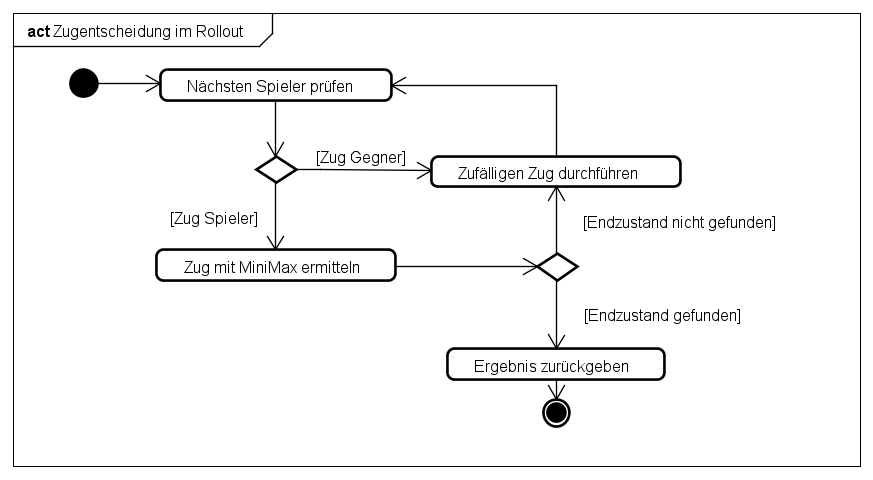
\includegraphics[scale=0.6]{pics/MR-activity.png}
\caption{Darstellung einer Zugentscheidung im Rollout des MCTS-MR}
\label{abb:mr-activiy}
\end{figure}

\textbf{MCTS-MS}: Hier ist die Selektion so angepasst, dass vor der Wahl des als nächsten zu selektierenden Knotens überprüft wird, ob dieser bereits ein bestimmtes Limit $l$ an Besuchen erreicht hat. Ist dies der Fall, wird eine MiniMax-Suche mit vorgegebener Tiefe $d_{mm}$ gestartet. Hierbei ist darauf zu achten, welcher der beiden Spieler der Maximierer ist. Falls das Ergebnis ein Sieg für den eigenen Spieler oder eine Niederlage für den Gegner darstellt, so wird das Ergebnis $r = 1$ gesetzt. Der eigene Spieler hat somit sicher die Chance zu gewinnen. Wird jedoch eine Niederlage für den eigenen Spieler oder ein Sieg für den Gegner gefunden, wird $r = -1$ vergeben. In diesem Fall hat der Gegner sicher die Chance zu gewinnen. Anschließend wird überprüft, ob dieses Ergebnis den tatsächlichen Wert $w$ des Knoten widerspiegelt. Sind $w$ und $r$ im Vorzeichen gleich, so wird $r$ zuerst über die Backpropagation bis zur Wurzel verbreitet. Anschließend erfolgt die Selektion des nächsten Kindknotens.\\\\\\\\
\textbf{MCTS-MB}: Die Umsetzung dieses Algorithmus wird in \autoref{abb:mb-activiy} dargestellt. Bevor die eigentliche Backpropagation erfolgt, wird in dieser Bachelorarbeit überprüft, ob der aktuell selektierte Knoten einen Endzustand des Spiels darstellt. Ist dies der Fall, so wird vor der MiniMax-Suche der $d_{mm}$-letzte Elternknoten des selektierten Knotens bei dem Start der MiniMax-Suche ausgewählt, um die Tiefe $d_{mm}$ komplett ausnutzen zu können. Als nächstes gilt es, anhand des Ergebnisses der MiniMax-Suche, Sieg oder Niederlage zu beweisen. Stellt der selektierte Knoten einen Sieg für den eigenen Spieler dar und die MiniMax-Suche ermittelt für den Gegner bestenfalls nur eine Niederlage, so ist der Sieg des eigenen Spielers bewiesen. Die eigene Niederlage gilt als bewiesen, falls der selektierte Knoten eine Niederlage darstellt und die MiniMax-Suche für den eigenen Spieler nur Niederlagen ermitteln kann. Anschließend erfolgt die normale Backpropagation anhand dieser Werte. Da sich diese Umsetzung nur auf gefundene Niederlagen der MiniMax-Suche fokussiert, wird bei einem Sieg der übliche Wert $w=1$ für die Backpropagation verwendet.

\begin{figure}[h]
\centering
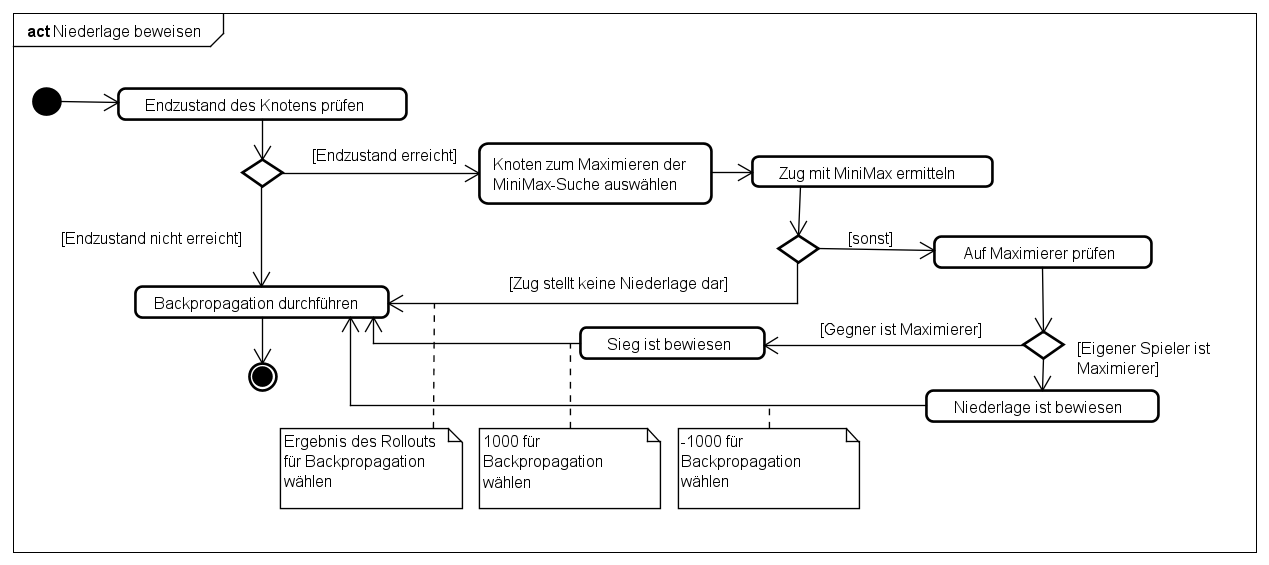
\includegraphics[scale=0.5]{pics/MB-activity.png}
\caption{Beweise in der Backpropagation des MCTS-MB}
\label{abb:mb-activiy}
\end{figure}

\textbf{MCTS-IPM}: Die Umsetzung orientiert sich nahe an der Erklärung aus Kapitel \ref{sec:mcts-hyb}. Es wird eine MiniMax-Suche mit der Tiefe $d_{mm}$ gestartet, wenn ein Knoten bereits eine bestimmte Anzahl an Besuchen erreicht hat. Das Ergebnis dieser Suche wird anschließend ohne weitere Überprüfung in dem Knoten gespeichert (siehe \autoref{eq:ipem}). Da dieser Hybrid-Algorithmus die Möglichkeit bereitstellen soll, zusätzlich Zugsortierung und K-Best-Pruning zu verwenden, wird für das Alpha-Beta-Pruning ein weiterer Spielbaum erstellt. Dieser Spielbaum wird nach dem Ermitteln des besten Zugs gelöscht. Aufgrund der Rechenzeit ist diese Umsetzung nicht optimal, aber durch die Zugsortierung bedingt notwendig.\\
%Hier erfolgt die MiniMax-Suche mittels einer Heuristik. Hierbei wird, wie bei MCTS-MS, bei einem erreichten Limit der Besuche der MiniMax gestartet. Anschließend wird der ermittelte Wert unter Berücksichtigung des vordefinierten Gewichts lediglich in dem gerade selektierten Knoten gespeichert. Eine Überprüfung der ermittelten Werte und der im Knoten befindenden Werte erfolgt hierbei nicht, um eine uneingeschränkte Umsetzung zum MCTS-MS zu vergleichen.
Da nun die Implementierung der Spielbaum-Algorithmen behandelt wurde, wird die Umsetzung des Alpha-Zero-Trainings erläutert.
\subsubsection{Implementierung des AlphaZero-Trainings}
Zu Beginn wird das neuronale Netz mit zufälligen Werten initialisiert. Anschließend erfolgt die Trainingsphase, wobei das neuronale Netz gegen sich selbst spielt. Die Zugwahl erfolgt hierbei ausschließlich mithilfe der Simulationen des MCTS-Algorithmus, wobei dieser nun die Wahrscheinlichkeiten des neuronalen Netzes berücksichtigt. Hierbei ist \autoref{eq:uct} wie folgt abgeändert:
\begin{align}
\text{UCT}_{AZ}(s, n) = \overline{X_{j}}(n) + p_{AZ}(s) \cdot 2C_{p} \cdot \sqrt{\frac{2 \cdot \ln{[v(n)]}}{v(n_{j})} }
\label{eq:az_new}
\end{align} 
Das neuronale Netz liefert unter der Angabe des aktuellen Spielfeldes $s$ eine Wahrscheinlichkeit $p_{AZ}(s)$, welche die Exploration des Spielbaums beeinflusst. Dies hat den positiven Effekt, dass das neuronale Netz nun die Exploration einzelner Knoten des Spielbaums kontrollieren kann. Ist beispielsweise ein Spielzug für das neuronale Netz unerforscht, so kann ein hohes $p_{AZ}(s)$ vergeben werden, wodurch dieser Zug im Spielbaum simuliert werden kann. Zusätzlich werden die Ergebnisse $w$ des Rollouts und $v$ des neuronalen Netzes addiert. Dieses Ergebnis wird anschließend für die Backpropagation eingesetzt. Die UCT-Suche wiederholt sich mit einer festgelegten Anzahl $s_{sim}$. Für das Training der Wahrscheinlichkeiten des neuronalen Netzes werden die Ergebnisse der MCTS-Simulationen verwendet. Hierfür wird alleinig das Verhältnis von $v$ zu $s_{sim}$ der jeweiligen Knoten benutzt. Dadurch wird dem Netz gezeigt, wie häufig die einzelnen Knoten in der UCT-Suche aufgesucht wurden. Nachdem ein Zug kalkuliert worden ist, werden das aktuelle Spielfeld, das Verhältnis aus der Anzahl der besuchten Züge während der Simulationen und der Parameter $w$, der Gewinne der Simulationen, gespeichert. Hierbei ist anzumerken, dass das aktuelle Spielfeld immer aus der Sicht des eigenen Spielers zum Training gegeben wird. Der eigene Spieler wird hierbei immer mit einer 1 dargestellt, wohingegen der Gegner als -1 dargestellt wird. Ist z.B. der gegnerische Spieler am Zug, so werden die Spieler auf dem Spielfeld invertiert, d.h. 1 wird zu -1 und umgekehrt, damit die Trainingsdaten immer aus der Sicht des aktuellen Spielers dargestellt werden. Wenn die maximale Anzahl an Simulationen erreicht ist, wird das gesammelte Spielgeschehen dem neuronalen Netz übergeben und dessen Parameter werden anschließend trainiert. Dieser gesamte Prozess wird auch in einer vorab definierten Anzahl an Trainingsiterationen $num_{train}$ wiederholt (siehe \autoref{abb:training-seq}).

\begin{figure}[h]
\centering
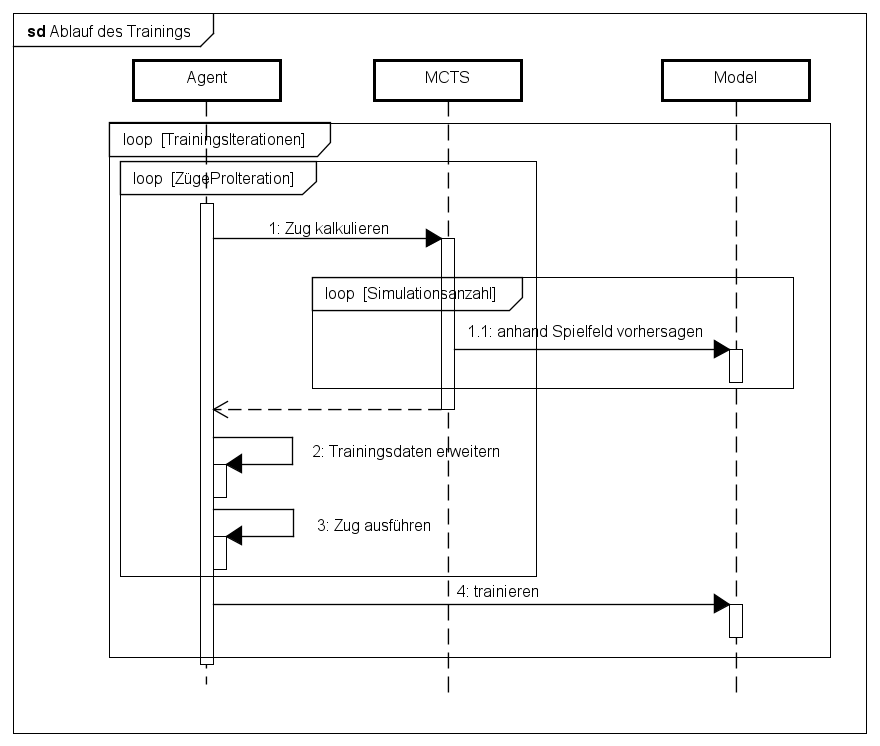
\includegraphics[scale=0.4]{pics/training.png}
\caption{Ablauf des Training}
\label{abb:training-seq}
\end{figure}

Ein simplifiziertes Beispiel eines Trainingsdatensatzes für den Ausschnitt eines Spielfelds ist in \autoref{abb:traindaten} dargestellt. Das Spielfeld zeigt hierbei den typischen Spielbeginn eines jeden Reversi-Spiels. In \autoref{abb:train-prob} ist das Feld mit den Koordinaten (4;1) 10-mal während den 50 MCTS-Simulationen besucht worden und bekommt deshalb den Wert 0,2 zugewiesen. Die Position (2;3) hingegen ist 20-mal besucht worden und bekommt infolge dessen den Wert 0,4. Die übrigen Felder werden analog berechnet, wobei Felder, auf die der Spieler nicht ziehen kann oder  die bereits eingenommen sind, mit einer 0 bewertet werden. Das Endergebnis der Simulationen ist in diesem Beispiel eine 1, folglich hat der Spieler gewonnen. Falls der Gegner in diesem Beispiel am Zug ist, würden in \autoref{abb:train-board} und \autoref{abb:train-prob} das Spielfeld aus dessen Sicht dargestellt werden, also die Werte 1 und -1 vertauscht werden.
% Table generated by Excel2LaTeX from sheet 'Tabelle1'
\begin{figure} [h]
\centering
\begin{minipage}[b]{0.25\linewidth}
\centering
\begin{tabular}{|c|c|c|c|c|c|}
\hline
0 & 0 & 0  & 0  & 0 & 0 \\ \hline
0 & 0 & 1  & -1 & 0 & 0 \\ \hline
0 & 0 & -1 & 1  & 0 & 0 \\ \hline
0 & 0 & 0  & 0  & 0 & 0 \\ \hline
\end{tabular}
\subcaption{Aktuelles Spielfeld}
\label{abb:train-board}
\end{minipage}
%\hspace{1.5cm}
\qquad
\begin{minipage}[b]{0.3\linewidth}
\centering
\begin{tabular}{|c|c|c|c|c|c|}
\hline
0 & 0   & 0   & 0,2 & 0   & 0 \\ \hline
0 & 0   & 0   & 0   & 0,3 & 0 \\ \hline
0 & 0,4 & 0   & 0   & 0   & 0 \\ \hline
0 & 0   & 0,1 & 0   & 0   & 0 \\ \hline
\end{tabular}
\subcaption{Verhältnisse der Besuche}
\label{abb:train-prob}
\end{minipage}
\qquad
\begin{minipage}[b]{0.3\linewidth}
	\centering
   \begin{tabular}{|r|}
    \hline
    1 \\
    \hline
    \end{tabular}%
  \label{tab:addlabel}%
\subcaption{Ergebnis der Simulation}
\label{abb:train-ergebnis}
\end{minipage}
\caption{Beispiel eines Trainingsdatensatzes}
\label{abb:traindaten}
\end{figure}
%Ist das Training abgeschlossen, so folgt die Evaluierung. Das neuronale Netz spielt hierbei gegen dessen vorherige Version, also vor dem letzten Training, an. Hierbei werden $num_{eval}$ Spiele gespielt. Auch hier erfolgt die Zugwahl anhand des MCTS-Algorithmus unter Berücksichtigung der gelieferten Wahrscheinlichkeiten zur jeweiligen Spielsituation.\\
%Sind alle $num_{eval}$ Evaluierungsspiele erfolgt, wird überprüft, ob das trainierte neuronale Netz   in mindestens $55\%$ der Spiele gewonnen hat. Ist dies der Fall, so wird das aktuell beste Model durch das trainierte Netz ersetzt. Andernfalls wird dieses verworfen.\\
%Dieses komplette Vorgehen wird $num_{total}$ wiederholt.\\
%\\Der Trainingsdatensatz nach Alpha Zero besteht aus kompletten Spiele. In \citep{Silver.05.12.2017} wird beschrieben, dass AlphaZero dessen Vorgänger übertrifft. Aufgrund dieser unterschiedlichen Trainingsmechanismen ist es interessant, diese Ansätze zu vergleichen.\\
%In dieser Arbeit erfolgt der zweite Trainingsansatz unter Verwendung des MCTS-Algorithmus, um Zugwahlen zu treffen. Jedoch wird nicht das Ergebnis der Simulationen gespeichert. Es werden Spiele von Anfang bis Ende gespielt, wobei die Spielpositionen und das erreichte Endergebnis zum Trainieren des neuronalen Netzes verwendet werden.\\ %Die Evaluierung des Models erfolgt ähnlich zum vorher genannten AlphaZero-Training.\\

\pagebreak
% ----------------------------------------------------------------------------------
% Kapitel: Evaluierung
% ----------------------------------------------------------------------------------
\section{Ergebnisse und Diskussion}
In diesem Kapitel werden die in den vorherigen Kapiteln erläuterten Algorithmen anhand von Versuchen evaluiert. Hierfür werden die Ergebnisse dieser Versuche dargestellt und diskutiert. Die Algorithmen treten gegen eine KI an, die mit Alpha-Beta-Pruning die Züge kalkuliert. Diese KI verwendet ausschließlich die Taktik, die höchste Anzahl an eigenen Steinen zu besitzen, unabhängig von der eigenen und gegnerischen Stabilität und Mobilität. Aus diesem Grund wird diese KI auch als gierig bezeichnet und im Folgenden \emph{triviale KI} genannt. Zu Beginn werden die bereits bekannten Heuristiken aus \autoref{sec:heuristik} bewertet, indem gegen die triviale KI gespielt wird. Die beste Heuristik wird im Folgenden für MCTS-IPM verwendet. Zusätzlich spielt der klassische MCTS gegen die triviale KI, um das Potential dieses Algorithmus zu prüfen. Anschließend treten die MCTS-Hybride aus \autoref{sec:mcts-hyb} gegen den klassischen MCTS und die triviale KI an. Abschließend wird das Ergebnis des neuronalen Netzes des AlphaZero-Ansatzes dargestellt und diskutiert.

\subsection{Die Wahl der Heuristik} \label{sec:wahl-heur}
Zunächst muss sich für eine Heuristik entschieden werden, die MCTS-IPM verwenden soll. Die Heuristik $h$ berücksichtigt Stabilität, Mobilität, die eigene Anzahl an Steinen und das statische Spielfeld gleichzeitig und berechnet sich bezogen auf das aktuelle Spielfeld $b$ und Spieler $s$ anhand des Mittelwerts dieser Eigenschaften:
\begin{align}
h(b, s) = \frac{w_{m}\cdot\text{TaM}(b) + w_{r}\cdot\text{Stab}(b) + w_{n}\cdot N(s) + w_{f}\cdot\text{StB}(s)}{4}
\end{align} 
Damit festgelegt werden kann, auf welche Spielfeldpositionen geachtet werden soll, werden die Werte der Stabilität, Mobilität, Anzahl an Steinen und statisches Spielfeld durch die Werte $w_i$ gewichtet. Dadurch kann festgelegt werden, ob die KI sich z.B. mehr auf die Stabilität oder auf die Anzahl der eigenen Steine fokussieren soll. Da jedoch kein gieriges Verhalten auftreten soll, wird $w_n$ vorzugsweise am niedrigsten Gewichtet. Des Weiteren wird kein dynamisches statisches Feld verwendet, was dazu führen kann, dass obwohl der eigene Spieler bereits eine Ecke eingenommen hat, die außenrum liegenden Felder trotzdem negativ bewertet werden und es somit dazu führen kann, dass der Spieler diese Felder nicht einnehmen will. Aufgrund dessen wird $w_{f}$ ebenfalls vorzugsweise niedrig gewertet. Wie in Kapitel \ref{sec:heuristik} bereits erläutert wird, sind Stabilität und Mobilität essentiell für die KI, um die eigene Einschränkung an Zügen und eine vorzeitige Niederlage vermeiden zu können, wodurch die Gewichte $w_{m}$ und $w_{r}$ am höchsten gesetzt werden.\\
Damit die vorherigen Aussagen überprüft werden und sich für eine Wahl der Gewichte für die Heuristik des MCTS-IPM entschieden werden kann, spielt der Client unter der Berücksichtigung einer Heuristik mit variierenden Gewichten wiederholend gegen die triviale KI. Da hierbei beide Parteien Alpha-Beta-Pruning verwenden und keine Zufallssimulationen durchgeführt werden, werden Spiele mit den selben Gewichten folglich immer gleich ausfallen. Wie der folgenden \autoref{tab:heur-gew} zu entnehmen ist, sind fünf Durchläufe pro MiniMax-Tiefe $d_{mm}$ geschehen, um die Wahl der optimalen Gewichte treffen zu können. Der Parameter $Z_{S}$ beschreibt die Anzahl an Zügen im Spiel bezogen auf den eigenen Spieler, wohingegen sich $Z_{G}$ analog auf den Gegner bezieht. Die Anzahl an besetzen Positionen des Spielers im Endzustand wird durch $N_{S}$ dargestellt. Die Anzahl an besetzten Ecken durch den eigenen Spieler wird durch $N_E$ beschrieben. Hat der eigene Spieler gewonnen, so wird dies durch $\text{Sieg}=1$ dargestellt. Andernfalls wird dies durch eine 0 ausgedrückt. Der Client hat hierbei, unter der Verwendung des Alpha-Beta-Pruning mit vorgegebener Spielbaumtiefe $d_{mm}$ gegen die triviale KI gespielt. Hierbei sind die Tiefen $d_{mm} \in \{1, 2, 3, 4, 5\}$ gewählt worden. Die Gewichte für die Bewertungsfunktion sind im Bereich $\{0.75, 1.0, 2.0\}$ definiert worden. Die triviale KI hat mit der selben vorgegebenen Tiefe für das Alpha-Beta-Pruning die Zugwahl getroffen.


\begin{table}[h]
  \centering
    \begin{tabular}{|rrrrrrrrrr|}
    \hline
    $d_{mm}$ & $Z_{S}$ & $Z_{G}$ & $N_{S}$ & $N_E$ & $w_f$ & $w_m$ & $w_r$ & $w_n$ & Sieg\\ [0.5ex]
    \hline\hline
    1     & 31    & 29    & 43    & 2     & 1\cellcolor[rgb]{ .949,  .949,  .949}     & 1\cellcolor[rgb]{ .949,  .949,  .949}     & 1\cellcolor[rgb]{ .949,  .949,  .949}     & 1\cellcolor[rgb]{ .949,  .949,  .949}     & 1\cellcolor[rgb]{ .949,  .949,  .949} \\
    1     & 30    & 30    & 44    & 4     & 0,75\cellcolor[rgb]{ .949,  .949,  .949}  & 0,75\cellcolor[rgb]{ .949,  .949,  .949}  & 0,75\cellcolor[rgb]{ .949,  .949,  .949}  & 2\cellcolor[rgb]{ .949,  .949,  .949}     & 1\cellcolor[rgb]{ .949,  .949,  .949} \\
    1     & 31    & 29    & 52    & 3     & 1\cellcolor[rgb]{ .949,  .949,  .949}     & 2\cellcolor[rgb]{ .949,  .949,  .949}     & 2\cellcolor[rgb]{ .949,  .949,  .949}     & 0,75\cellcolor[rgb]{ .949,  .949,  .949}  & 1\cellcolor[rgb]{ .949,  .949,  .949} \\
    1     & 32    & 28    & 39    & 3     & 2\cellcolor[rgb]{ .949,  .949,  .949}     & 0,75\cellcolor[rgb]{ .949,  .949,  .949}  & 0,75\cellcolor[rgb]{ .949,  .949,  .949}  & 0,75\cellcolor[rgb]{ .949,  .949,  .949}  & 1\cellcolor[rgb]{ .949,  .949,  .949} \\
    1     & 33    & 27    & 39    & 2     & 1\cellcolor[rgb]{ .949,  .949,  .949}     & 0,75\cellcolor[rgb]{ .949,  .949,  .949}  & 2\cellcolor[rgb]{ .949,  .949,  .949}     & 0,75\cellcolor[rgb]{ .949,  .949,  .949}  & 1\cellcolor[rgb]{ .949,  .949,  .949} \\
    \hline
    2     & 31    & 29    & 32    & 3     & 1     & 1     & 1     & 1     & 0 \\
    2     & 31    & 29    & 46    & 4     & 0,75\cellcolor[rgb]{ .949,  .949,  .949}  & 0,75\cellcolor[rgb]{ .949,  .949,  .949}  & 0,75\cellcolor[rgb]{ .949,  .949,  .949}  & 2\cellcolor[rgb]{ .949,  .949,  .949}     & 1\cellcolor[rgb]{ .949,  .949,  .949} \\
    2     & 31    & 29    & 34    & 3     & 1\cellcolor[rgb]{ .949,  .949,  .949}     & 2\cellcolor[rgb]{ .949,  .949,  .949}     & 2\cellcolor[rgb]{ .949,  .949,  .949}     & 0,75\cellcolor[rgb]{ .949,  .949,  .949}  & 1\cellcolor[rgb]{ .949,  .949,  .949} \\
    2     & 32    & 28    & 49    & 3     & 2\cellcolor[rgb]{ .949,  .949,  .949}     & 0,75\cellcolor[rgb]{ .949,  .949,  .949}  & 0,75\cellcolor[rgb]{ .949,  .949,  .949}  & 0,75\cellcolor[rgb]{ .949,  .949,  .949}  & 1\cellcolor[rgb]{ .949,  .949,  .949} \\
    2     & 34    & 25    & 56    & 3     & 1\cellcolor[rgb]{ .949,  .949,  .949}     & 0,75\cellcolor[rgb]{ .949,  .949,  .949}  & 2\cellcolor[rgb]{ .949,  .949,  .949}     & 0,75\cellcolor[rgb]{ .949,  .949,  .949}  & 1\cellcolor[rgb]{ .949,  .949,  .949} \\
    \hline
    3     & 30    & 30    & 12    & 2     & 1     & 1     & 1     & 1     & 0 \\
    3     & 30    & 30    & 17    & 2     & 0,75  & 0,75  & 0,75  & 2     & 0 \\
    3     & 31    & 29    & 46    & 4     & 1\cellcolor[rgb]{ .949,  .949,  .949}     & 2\cellcolor[rgb]{ .949,  .949,  .949}     & 2\cellcolor[rgb]{ .949,  .949,  .949}     & 0,75\cellcolor[rgb]{ .949,  .949,  .949}  & 1\cellcolor[rgb]{ .949,  .949,  .949} \\
    3     & 32    & 28    & 45    & 2     & 2\cellcolor[rgb]{ .949,  .949,  .949}     & 0,75\cellcolor[rgb]{ .949,  .949,  .949}  & 0,75\cellcolor[rgb]{ .949,  .949,  .949}  & 0,75\cellcolor[rgb]{ .949,  .949,  .949}  & 1\cellcolor[rgb]{ .949,  .949,  .949} \\
    3     & 33    & 27    & 59    & 4     & 1\cellcolor[rgb]{ .949,  .949,  .949}     & 0,75\cellcolor[rgb]{ .949,  .949,  .949}  & 2\cellcolor[rgb]{ .949,  .949,  .949}     & 0,75\cellcolor[rgb]{ .949,  .949,  .949}  & 1\cellcolor[rgb]{ .949,  .949,  .949} \\
    \hline
    4     & 28    & 32    & 3     & 0     & 1     & 1     & 1     & 1     & 0 \\
    4     & 31    & 29    & 24    & 1     & 0,75  & 0,75  & 0,75  & 2     & 0 \\
    4     & 31    & 29    & 50    & 3     & 1\cellcolor[rgb]{ .949,  .949,  .949}     & 2\cellcolor[rgb]{ .949,  .949,  .949}     & 2\cellcolor[rgb]{ .949,  .949,  .949}     & 0,75\cellcolor[rgb]{ .949,  .949,  .949}  & 1\cellcolor[rgb]{ .949,  .949,  .949} \\
    4     & 31    & 29    & 46    & 3     & 2\cellcolor[rgb]{ .949,  .949,  .949}     & 0,75\cellcolor[rgb]{ .949,  .949,  .949}  & 0,75\cellcolor[rgb]{ .949,  .949,  .949}  & 0,75\cellcolor[rgb]{ .949,  .949,  .949}  & 1\cellcolor[rgb]{ .949,  .949,  .949} \\
    4     & 31    & 29    & 21    & 2     & 1     & 0,75  & 2     & 0,75  & 0 \\
    \hline
    5     & 23    & 25    & 3     & 1     & 1     & 1     & 1     & 1     & 0 \\
    5     & 30    & 30    & 29    & 2     & 0,75  & 0,75  & 0,75  & 2     & 0 \\
    5     & 30    & 30    & 26    & 2     & 1     & 2     & 2     & 0,75  & 0 \\
    5     & 31    & 29    & 12    & 2     & 2     & 0,75  & 0,75  & 0,75  & 0 \\
    5     & 30    & 30    & 12    & 2     & 1     & 0,75  & 2     & 0,75  & 0 \\
    \hline
    \end{tabular}%
    \caption{Spielergebnisse der variierenden Heuristik gegen die triviale KI}
  \label{tab:heur-gew}%
\end{table}%
In \autoref{tab:heur-gew} ist deutlich zu sehen, dass bei einheitlichen Gewichten $w_i=1$, der betrachtete Spieler bei steigender Spielbaumtiefe schlechter wird. Es können hierbei nur Spiele mit einer Tiefe von $d_{mm}=1$ gewonnen werden. Auch ist deutlich zu erkennen, dass bei steigender Tiefe immer weniger Heuristiken gewinnen und die triviale KI somit stärker wird. Wie bei $d_{mm}=4$ zu sehen ist, reicht es ab dieser Tiefe nicht mehr aus, hauptsächlich die Ecken des Spielfeldes belegen zu wollen. In den Fällen $d_{mm} \in \{1;2;3;4\}$ ist zu sehen, dass die Ergebnisse der Kombination $(1.0, 2.0, 2.0, 0.75)$, also das Fokussieren auf die Mobilität der eigenen Steine und belegten Ecken, vielversprechend ausfallen. Das Selbe gilt für die Kombination $(2; 0,75; 0,75; 0,75)$, wobei der Hauptfokus auf dem statischen Feld liegt. Womit bestätigt wird, dass beide Bewertungsfunktionen eine gute Wahl für die Heuristik des MCTS-IPM sind. Jedoch ist auch erkennbar, dass ab einer Spielbaumtiefe von $t_{mm}=5$ diese Ansätze zur Berechnung der Heuristik nicht mehr ausreichen. Anhand dieser Tiefe ist gut zu erkennen, dass zwei besetzte Ecken nicht ausreichen, um das Spiel zu gewinnen und hierbei eine bessere Strategie notwendig ist. 
\subsection{MCTS gegen triviale KI}
Um den klassischen MCTS zu prüfen, spielt auch dieser gegen die triviale KI. Es werden hierbei je 100 Spiele mit einer Simulationsanzahl $s_{sim} \in \{50; 100; 150; 200\}$ gegen die triviale KI mit einer  Spielbaumtiefe $d_{mm} \in \{1;2;3;4;5\}$ durchgeführt. Die Ergebnisse der Versuche sind in der folgenden \autoref{abb:mcts-triv-erg} dargestellt. Im Folgenden wird die MCTS-Suche mit $s_{sim}=X$ als MCTS-$X$ abgekürzt. 

\begin{figure} [h]
%\centering
\begin{minipage}[b]{0.45\linewidth}
\centering
\begin{tikzpicture}
\begin{axis}[
	height=7.5cm,
	axis lines = left,
	xmax=5.5,
	xmin=0,
	xtick={0,1,...,5},
	xlabel=$d_{mm}$,
	ymax=1.05,
	ymin=0.25,
	ytick={0.25,0.5,...,1},
	%ylabel=$s_{sim}$,
	legend style={at={(0.6,.5)},anchor=north west},
	]
	\addplot[solid] table [x=i,y=mc-50]{winrate_mcvtriv.dat};
	\addplot[red, solid] table [x=i,y=mc-100]{winrate_mcvtriv.dat};
	\addplot[blue, solid] table [x=i,y=mc-150]{winrate_mcvtriv.dat};
	\addplot[brown, solid] table [x=i,y=mc-200]{winrate_mcvtriv.dat};
	\addlegendentry{mcts-50}
	\addlegendentry{mcts-100}
	\addlegendentry{mcts-150}
	\addlegendentry{mcts-200}

\end{axis}
\end{tikzpicture}
\subcaption{Siegesrate}
\label{abb:mcts-win}
\end{minipage}
%\hspace{1.5cm}
\hfill
\begin{minipage}[b]{0.45\linewidth}
\centering
\begin{tikzpicture}
\begin{axis}[
	width=7cm,
	height=7.5cm,
	axis lines = left,
	xlabel=$s_{sim}$,
	xmax=210,
	xmin=0,
	xtick={0,50,100,150,200},
	ymax=150,
	ymin=0,
	ylabel=$\overline{t}\text{ in ms}$,
	ytick={0,50,...,100},
	]
	\addplot[solid] table [x=i,y=mc]{runtime_mctstriv.dat};
\end{axis}
\end{tikzpicture}
\subcaption{Durchschnittliche Rechenzeit pro Zug}
\label{abb:mcts-runtime}
\end{minipage}
\caption{Ergebnisse von MCTS gegen triviale KI}
\label{abb:mcts-triv-erg}
\end{figure}

In \autoref{abb:mcts-win} ist zu erkennen, dass bereits mit einer Simulationsanzahl von $s_{sim} = 50$ sehr gute Ergebnisse erzielt werden können. Sogar bei einer MiniMax-Tiefe von $t_{mm} = 5$ können 73 von 100 Spielen gewonnen werden, obwohl hierbei die Heuristiken aus \autoref{tab:heur-gew} ihre Grenzen erreichen. Die durchschnittliche Regenzeit pro Zug erfolgt bereits mit einer durchschnittlichen Berechnungszeit von 28,6 ms pro Zug. Mit steigender Simulationsanzahl steigt auch die Siegesrate pro MiniMax-Tiefe. Vor allem ist der Unterschied zwischen $s_{sim} = 200$ zu $s_{sim} = 50$ an der Stelle $d_{mm} = 5$ deutlich bemerkbar. An den Stellen $d_{mm} = 1$ bis $d_{mm} = 4$ ist auch zu erkennen, dass eine Simulationsanzahl von $s_{sim} = 100$ im Vergleich zu den höheren $s_{sim}$ annähernd die selbe Anzahl an Siege erbringt. Der Verlauf der Zeit zur Zugberechnung nimmt hierbei einen annähernd linearen Verlauf an, wobei für $s_{sim} = 200$ durchschnittlich 99,97 ms an Rechenzeit pro Zug benötigt wird. An diesen Ergebnissen ist zu erkennen, dass bei steigender MiniMax-Tiefe eine steigende Anzahl an Simulationen für den MCTS-Algorithmus durchaus sinnvoll ist. Die durchschnittliche Zeit pro Zugberechnung ist hierbei annähernd proportional zur Simulationsanzahl.

\subsection{MCTS-Keep gegen klassischen MCTS}
Um die Verbesserung des MCTS-Algorithmus aus \autoref{sec:optimi} zu verifizieren, spielt ein MCTS-Algorithmus, unter Verwendung der Optimierungen, gegen den herkömmlichen MCTS. Hierbei werden insgesamt 800 Spiele gespielt, wobei die Anzahl der Simulationen $s_{sim}\in \{50;100;150;200\}$ nach 200 Spielen variiert wird.\\
Wie in \autoref{abb:mctskeepwin} zu erkennen ist, ist MCTS-Keep nicht signifikant besser als seine klassische Version, wenn nur die Siegesrate betrachtet wird. Auffallend ist das annähernd lineare Verhalten von $s_{sim}$ und die durchschnittliche Anzahl an Besuchen der übernommenen Knoten $\overline{v}$ pro Spiel. Zum Beispiel beträgt bei einer Simulationsanzahl von $s_{sim} = 50$ die Gesamtanzahl an Besuchen von wiederverwendeten Knoten ca. 46,53 pro Spiel. Durch \autoref{abb:mctskeepvisits} ist somit anzunehmen, dass $s_{sim}$ und $\overline{v}$ proportional zueinander sind.

\begin{figure} [h]
\centering
\begin{minipage}{0.4\textwidth}
\centering
\begin{tikzpicture}
\begin{axis}[
	height=7.5cm,
	width=7cm,
	axis lines = left,
	xmax=210,
	xmin=0,
	xtick={0,50,100,150,200},
	xlabel=$s_{sim}$,
	ymax=1.05,
	ymin=0,
	ytick={0,0.25,...,1},
	]
	\addplot[solid] table [x=i,y=win]{mctskeeptree.dat};
\end{axis}
\end{tikzpicture}
\subcaption{Siegesrate}
\label{abb:mctskeepwin}
\end{minipage}
\qquad
\begin{minipage}{0.4\textwidth}
\centering
\begin{tikzpicture}
\begin{axis}[
	height=7.5cm,
	width=7cm,
	axis lines = left,
	xmax=210,
	xmin=0,
	xtick={0,50,100,150,200},
	xlabel=$s_{sim}$,
	ymax=300,
	ymin=0,
	ytick={0,50,...,250},
	ylabel=$\overline{v}$
	]
	\addplot[solid] table [x=i,y=node]{mctskeeptree.dat};
	%\addlegendentry{$\overline{v}$}
\end{axis}
\end{tikzpicture}
\subcaption{$\overline{v}$ übernommener Knoten pro Spiel}
\label{abb:mctskeepvisits}
\end{minipage}
\label{abb:mctskeeptotal}
\caption{Ergebnisse von MCTS-Keep gegen MCTS}
\end{figure}
Somit lässt sich schlussfolgern, dass die Beibehaltung des Spielbaums besonders hilfreich für MCTS-MS uns MCTS-IPM ist, da diese Hybride anhand der Anzahl an Besuchen pro Knoten die MiniMax-Suche starten.

\subsection{Analyse der MCTS-Hybriden}
Um die Verbesserung der Kombinationen aus MCTS und MiniMax gegenüber dem herkömmli-chen MCTS überprüfen zu können, spielen diese Algorithmen gegeneinander. Hierbei können verschiedene Parameter der Algorithmen verändert werden, wodurch das Ermitteln einer einheitlichen Metrik erschwert wird.\\
Alle Algorithmen verwenden eine definierte Anzahl an Simulationen $s_{sim}$, also die Wiederholungen der Schritte Selektion bis Backpropagation, und den Parameter $c_{p}$, welcher die Exploration im Spielbaum beeinflusst. Im Folgenden wird $c_{p} = 0,75$ definiert, um das Ausmaß der Exploration zu limitieren. Hinzukommend verwenden die Hybride die Tiefe $d_{mm}$ für die MiniMax-Suche mit der Erweiterung Alpha-Beta-Pruning.\\
Aufbauend dazu verwenden MCTS-MS und MCTS-IPM zusätzlich den Parameter $l$ für das Limit zum Starten der MiniMax-Suche in der Selektion. MCTS-IPM verwendet zusätzlich das Gewicht $\gamma$, mit dem die Backpropagation beeinflusst wird, und die Heuristik $h$, welche in der MiniMax-Suche verwendet wird. Hierbei sei erneut angemerkt, dass MCTS-IPM der einzige Hybrid ist, der zusätzlich zum Alpha-Beta-Pruning die Zugsortierung und die Anzahl $k$ für das K-Best-Pruning verwendet.\\
Im Folgenden werden die Ergebnisse der MCTS-Hybride gegen den herkömmlichen MCTS verglichen. Hierbei wird der Spielbaum nach jeder neuen Zugaufforderung übernommen. Es erfolgen $s_{sim} = 100$ Simulationen und die MiniMax-Tiefe $d_{mm} = \{1, 2, 3, 4\}$ wird variiert. Anschließend werden die Attribute der Läufe verglichen. Generell werden Anzahl an eingenommenen Ecken, Siegesrate, Anzahl an Steinen am Ende des Spiels und Rechenzeit pro Zug analysiert. Hinzukommend werden Anzahl bewiesener Siege und Niederlagen, Ergebnis der Rollouts und Anzahl an Zügen pro Spiel in die Analyse aufgenommen. Die Algorithmen MCTS-MS und MCTS-IPM werden noch auf die Anzahl erreichter Limits pro Spiel untersucht, wobei die Limits variiert werden. Da als Abbruchbedingung der UCT-Suche ein bewiesener Sieg eines Kindknotens der Wurzel genügt und auf eine bewiesenen Niederlage hierbei nicht geachtet wird, sei hier bereits vorweggenommen, dass die Anzahl an bewiesenen Niederlagen die Siege übersteigen wird. Zuerst folgt die Darstellung der Ergebnisse für MCTS-MR.

\textbf{MiniMax im Rollout}: Da die MiniMax-Suche in jedem Schritt für die Zugentscheidung im Rollout verwendet wird, ist eine hohe Tiefe $d_{mm}$ sehr zeitaufwendig. Werden $100$ Simulationen und $d_{mm}=4$ gewählt, so dauert dies zur Berechnung eines einzigen Zugs durchschnittlich 5,1 s. Nimmt $d_{mm}=1$ an, reduziert dies die Rechenzeit auf 0,3 ms. Dies hat auch zur Folge, dass nur Endzustände in direkt folgenden Zügen entdeckt werden können. Bei einer höheren Spielbaumtiefe können Endzustände dementsprechend früher gefunden werden, sind jedoch rechenaufwändiger.Am besten hat hier MCTS-MR mit $t=3$ mit einer Siegesrate von 51\% abgeschlossen (siehe \autoref{abb:mr-win}). Die durchschnittliche Summen der Ergebnisse aus den Rollouts variieren hierbei bei den Tiefen $d_{mm}=\{1;2;4\}$ mit $\overline{N}_{roll}=\{120; 114; 104\}$. Die Tiefe $d_{mm}=3$ hat hierbei eine Auffälligkeit mit $\overline{N}_{roll}=-8$. Aufgrund der Ergebnisse der anderen MiniMax-Tiefen ist jedoch anzunehmen, dass dies ein Ausreißer ist.

\begin{figure} [h]
\centering
\begin{minipage}[t]{0.4\textwidth}
\centering
\begin{tikzpicture}
\begin{axis}[
	height=7.5cm,
	width=7cm,
	axis lines = left,
	xmax=4.5,
	xmin=0,
	xlabel=$d_{mm}$,
	xtick={0,1,...,4},
	ymax=1.05,
	ymin=0,
	ytick={0,0.25,...,1},
	]
	\addplot[solid] table [x=i,y=mr]{winrate.dat};
\end{axis}
\end{tikzpicture}
\subcaption{Siegesrate}
\label{abb:mr-win}
\end{minipage}
\qquad
\begin{minipage}[t]{0.4\textwidth}
\centering
\begin{tikzpicture}
\begin{axis}[
	height=7.5cm,
	width=7cm,
	axis lines = left,
	xmax=4.5,
	xmin=0,
	xtick={0,1,...,4},
	xlabel=$d_{mm}$,
	ymax=5.5,
	ymin=0,
	ytick={0,1.0,...,5.5},
	ylabel=$\overline{t}\text{ in s}$,
	legend style={at={(0.65,.9)},anchor=north west},
	]
	\addplot[solid] table [x=i,y=mr]{runtime.dat};
\end{axis}
\end{tikzpicture}
\subcaption{Durchschnittliche Rechenzeit pro Zug}
\label{abb:mr-else}
\end{minipage}

\caption{Ergebnisse von MCTS-MR gegen MCTS}
\label{abb:win_mr}
\end{figure}
Auffällig sind hier die Zeiten zur Zugberechnung. Die Rechenzeit hat sich ungefähr um den Faktor 19,5 erhöht. Aufgrund des angesprochenen Ausreißers bei $d_{mm}=3$ ist festzustellen, dass keine eindeutige Aussage bezogen zur Tiefe der MiniMax-Suche und dem Ergebnis der Rollouts gemacht werden kann. Es ist definitiv zu sehen, dass bei ca. 2900 Simulationen pro Spiel, nicht signifikant mehr Siege als Niederlagen festgestellt werden. 
%Es kann jedoch auf jeden Fall angenommen werden, bei durchschnittlich 29 Zügen pro Spiel mit 100 Simulationen, was ca. 2900 Simulationen pro Spiel (abgezogen der Einsparungen durch die Abbruchbedingung des MCTS-Solvers im späten Spielverlauf), dass nicht signifikant mehr Siege als Niederlagen in den Rollouts festgestellt werden. 
Aufgrund der Laufzeit und des Spielergebnisses ist hier $d_{mm}=1$ gegenüber $d_{mm}=4$ vorzuziehen. Abschließend ist anzunehmen, dass dieser Hybrid-Algorithmus nicht signifikant besser als seine klassische Version ist.\\
%Anschließend werden die Ergebnisse von MCTS-MS dargestellt und erläutert.
\textbf{MiniMax in der Selektion}: 
%Hier ist darauf zu achten, dass bei der Wahl des Limits $l$ kein zu niedriger Wert gewählt wird, da dies sonst dazu führt, dass in annähernd jedem Selektionsschritt eine MiniMax-Suche gestartet wird. Bei einem zu hohen Wert z.B. $l = 200$ bei einer Simulationsanzahl $s=150$, kann es dazu kommen, dass die MiniMax-Suche hingegen nicht gestartet wird und sich MCTS-MS somit wie MCTS-Solver verhält. Wird jedoch die Optimierung aus Kapitel \ref{sec:optimi} verwendet, d.h. dass der Spielbaum für das gesamte Spiel beibehalten wird, so wirkt sich ein hohes Limit nicht mehr insofern negativ auf den Hybriden aus, also dass der MiniMax-Algorithmus nicht mehr ausgeführt wird.\\
In \autoref{abb:ms-erg} werden die Ergebnisse mit den Limits $l=\{20;50\}$ gegen den klassischen MCTS dargestellt. Hierbei hat MCTS-MS-50 mit einer MiniMax-Tiefe von 1 das beste Ergebnis mit 106 Siegen erreicht. Die restlichen MiniMax-Tiefen haben hierbei nicht signifikant schlechtere Ergebnisse erzielt. Durchschnittlich ist das Limit der Knoten bei $l=50$ ca. 1500 mal erreicht und die MiniMax-Suche anschließend gestartet worden. Wegen der in der Tiefe ansteigenden MiniMax-Suche, erhöht sich die Zeit zur Zugberechnung bei $d_{mm}=1$ mit 0,07 s auf 1,8 s bei $d_{mm}=4$.\\
Bei der Wahl $l=20$ ist dieses Limit durchschnittlich 2100-mal erreicht worden. Aufgrund der vermehrten Anzahl an MiniMax-Suchen mit steigender Tiefe, erhöht sich auch hier die durchschnittliche Laufzeit zur Zugberechnung von 0,07 s bei $d_{mm}=1$ auf 2,1 s bei $d_{mm}=4$ (siehe \autoref{abb:ms-zeit}). Die Siegesrate fällt hier jedoch, im Vergleich zu $l=50$, nur für die Tiefen $d_{mm} = \{2;3\}$ ein wenig besser aus.\\
\begin{figure} [h]
\centering
\begin{minipage}[t]{0.4\textwidth}
\centering
\begin{tikzpicture}
\begin{axis}[
	height=7.5cm,
	width=7cm,
	axis lines = left,
	xmax=4.5,
	xmin=0,
	xlabel=$d_{mm}$,
	xtick={0,1,...,4},
	ymax=1.05,
	ymin=0,
	ytick={0,0.25,...,1},
	]
	\addplot[solid] table [x=i,y=ms-50]{winrate.dat};
	\addplot[red, solid] table [x=i,y=ms-20]{winrate.dat};
	%\node [right, black] at (axis cs: 0.5,0.9) {$\overline{t}_{Limits} \approx 1500$};
	\addlegendentry{$l=50$}
	\addlegendentry{$l=20$}
\end{axis}
\end{tikzpicture}
\subcaption{Siegesrate}
\label{abb:ms-win}
\end{minipage}
\qquad
\begin{minipage}[t]{0.4\textwidth}
\centering
\begin{tikzpicture}
\begin{axis}[
	height=7.5cm,
	width=7cm,
	axis lines = left,
	xmax=4.5,
	xmin=0,
	xtick={0,1,...,4},
	xlabel=$d_{mm}$,
	ymax=5.5,
	ymin=0,
	ytick={0,1.0,...,5.5},
	ylabel=$\overline{t}\text{ in s}$,
	]
	\addplot[solid] table [x=i,y=ms-50]{runtime.dat};
	\addplot[red, solid] table [x=i,y=ms-20]{runtime.dat};
	\addlegendentry{$l=50$}
	\addlegendentry{$l=20$}
\end{axis}
\end{tikzpicture}
\subcaption{Durchschnittliche Zeit zur Zugberechnung}
\label{abb:ms-zeit}
\end{minipage}
\caption{Ergebnisse von MCTS-MS-20 und MCTS-MS-50 gegen MCTS}
\label{abb:ms-erg}
\end{figure}
Aufgrund nahezu identischer Siegesraten ist daher anzunehmen, dass die Wahl des Limits mit $l=20$ oder $l=50$ keinen signifikanten Unterschied darstellt. Sogar in der Laufzeit zur Zugberechnung wirkt sich die Wahl $l=20$ nicht signifikant aus. Auch dieser Hybrid ist, aufgrund der Siegesraten, nicht auffallend besser als der klassische MCTS-Algorithmus. Um den Einfluss der Optimierung MCTS-Keep, den Spielbaum der MCTS-Simulationen das Spiel über beizubehalten, zu überprüfen, wird bei MCTS-IPM auf diese Optimierung verzichtet.\\
%Anschließend werden die Ergebnisse von MCTS-MB erläutert. Dies ist der letzte zu behandelnde Hybrid-Algorithmus, der keine Heuristiken verwendet.
\textbf{MiniMax in der Backpropagation}: Dieser Hybrid-Algorithmus hat, wie in \autoref{abb:win_mb} zu sehen ist, nur für die MiniMax-Tiefe $d_{mm} = 2$ den klassischen MCTS in mehr als $50\%$ der Spiele geschlagen. Die Wahl von $d_{mm} = 2$ hat hierbei das beste Ergebnis mit einer Siegesrate von $60\%$ erreicht und hat im Schnitt 6,35 Siege beweisen können. Durchschnittlich hat dieser Algorithmus 5,5 Siege und 333,1 Niederlagen pro Spiel bewiesen. Alle Versionen der MiniMax-Suche haben im Schnitt 58,8 ms für eine Zugentscheidung benötigt.

\begin{figure} [h]
\centering
\begin{tikzpicture}
\begin{axis}[
	axis lines = left,
	xmax=4.5,
	xmin=0,
	xtick={0,1,...,4},
	xlabel=$d_{mm}$,
	ymax=1.05,
	ymin=0,
	ytick={0,0.25,...,1},
	]
\addplot[solid] table [x=i,y=mb]{winrate.dat};
\end{axis}
\end{tikzpicture}
\caption{Siegesrate von MCTS-MB gegen MCTS}
\label{abb:win_mb}
\end{figure}
Die Umsetzung dieses Hybrid-Algorithmus stellt im Vergleich zu den vorherigen MCTS-Hybri-den, nicht mehr Siege sicher, obwohl das Beweisen von Siegen und Niederlagen und somit die Verbesserung des MCTS-Solver die Hauptaufgabe dieses Algorithmus ist. Die genauen Zahlen hierfür folgen am Ende dieses Abschnitts, da sich die Hybrid-Algorithmen im Beweisen der Siege und Niederlagen sehr ähnlich sind. Was diesen MCTS-Hybriden hinsichtlich seiner Ergebnisse von den vorherigen Algorithmen unterscheidet, ist die Rechenzeit pro Zug bei steigender MiniMax-Tiefe. Dies lässt sich darin begründen, dass MiniMax nur bei Knoten, die Endzustände repräsentieren, angewendet wird.\\
%Abschließend werden die Ergebnisse zu MCTS-IPM dargestellt.
\textbf{MiniMax mit Informierten Prior}: Da dieser Hybrid auf MCTS-MS basiert und sich lediglich in der Art der Verarbeitung und der ermittelten Ergebnisse des MiniMax unterscheiden, wirkt sich die Wahl des Limits höchstwahrscheinlich genauso aus, wie im vorherigen Abschnitt. 
%Hinzukommend ist herauszufinden, ob sich die Wahl der Gewichte für die Heuristik für diesen Algorithmus gravierend für die Zugentscheidung des MCTS-Algorithmus ausfällt. Falls z.B. die Heuristik sich mehr auf das Belegen von Ecken fokussiert, ist herauszufinden, ob sich der MCTS-IPM dementsprechend verhält, da das Ergebnis der Bewertungsfunktion nun zum Wert $w$ des Knotens addiert wird. 
Als Heuristik wird sich hierfür in allen Fällen der MiniMax-Tiefen für die Heuristik mit der Gewichtkombination $(1;2;2;0,75)$, d.h. Ecken zu besitzen und die eigene Mobilität sind die Hauptziele der Heuristik, entschieden. Das Knotengewicht wird hierbei mit $\gamma = 10$ gewählt. Aufgrund der vorangegangen Ergebnisse des MCTS-MS wird sich für das Limit $l=50$ entschieden. Zusätzlich werden während der MiniMax-Suche Zugsortierung und K-Best-Pruning mit $K = 3$ verwendet. Die Spielbäume, welche aus den MCTS-Simulationen entstehen, werden für diesen Versuch nicht übernommen, um zu überprüfen, ob dadurch die Limits signifikant weniger erreicht werden und dies eine Auswirkung auf die weiteren Ergebnisse hat. Die Ergebnisse sind in \autoref{abb:win_ipem} dargestellt. Hierbei ist das Limit durchschnittlich ca. 1400 mal pro Spiel erreicht worden. Da hierbei zur MiniMax-Suche ein weiterer Spielbaum aufgebaut und anschießend gelöscht wird, erhöht sich die Rechenzeit pro Zug erheblich von 0,07 s ($d_{mm}=1$) auf 13,1 s ($d_{mm}=4$). 

\begin{figure} [h]
\centering

\begin{minipage}{0.4\linewidth}
\begin{tikzpicture}
\begin{axis}[
	height=7.5cm,
	width=7cm,
	axis lines = left,
	xmax=4.5,
	xmin=0,
	xtick={0,1,...,4},
	xlabel=$d_{mm}$,
	ymax=1.05,
	ymin=0,
	ytick={0,0.25,...,1},
	]
\addplot[solid] table [x=i,y=ip-50]{winrate.dat};
\end{axis}
\end{tikzpicture}
\subcaption{Siegesrate}
\end{minipage}
\qquad
\begin{minipage}{0.4\linewidth}
\begin{tikzpicture}
\begin{axis}[
	height=7.5cm,
	width=7cm,
	axis lines = left,
	xmax=4.5,
	xmin=0,
	xtick={0,1,...,4},
	xlabel=$d_{mm}$,
	ymax=14,
	ymin=0,
	ytick={0,5,...,13},
	ylabel=$\overline{t}\text{ in s}$,
	]
	\addplot[solid] table [x=i,y=ip-50]{runtime.dat};
\end{axis}
\end{tikzpicture}
\subcaption{Durchschnittliche Zeit zur Zugberechnung}
\end{minipage}
\caption{Ergebnisse von IPEM-50 gegen MCTS}
\label{abb:win_ipem}
\end{figure}
Auffällig ist hier, dass die Ecken durchschnittlich nur 2,04-mal besetzt worden sind, obwohl die Heuristik auf diese Postionen achtet. Dies lässt vermuten, dass die Ergebnisse aus den Rollouts einen höheren Einfluss haben als die verwendete Heuristik. Da sich das Limit hier nur um eine Differenz von ca. 100 zu MCTS-MS-50 unterscheidet, ist festzustellen, dass die Optimierung von MCTS-Keep keinen Mehrwert für MCTS-MS und MCTS-IPM aufweist. Im Folgenden werden Gemeinsamkeiten der Kombinationen aus MCTS und MiniMax dargestellt.

\textbf{Auffällige Gemeinsamkeiten der MCTS-Hybride}: Auffällig ist das Besetzen der Eckpositionen. Es sind im Durchschnitt 2,01 Ecken pro Spiel besetzt worden. Ein weiteres Merkmal ist das Beweisen von Siegen und Niederlagen. Hierbei sind durchschnittlich 297,9 Niederlagen und 6,04 Siege pro Spiel bewiesen worden. Außerdem werden die Spiele, mit durchschnittlich 29,8 Zügen und ca. 31,7 belegten Feldern pro Spiel, nicht vorzeitig verloren. Was die steigende Tiefe der MiniMax-Suche betrifft, so ist aufgrund der Ergebnisse festzustellen, dass eine tiefere MiniMax-Suche die Siegesrate nicht verbessert. Hinzu kommt, dass eine steigende MiniMax-Tiefe die Zugberechnungszeit deutlich erhöht, wobei MCTS-MB aufgrund der Umsetzung aus \autoref{sec:umsetzung} hierbei eine Ausnahme darstellt.

\textbf{Hybride gegen triviale KI}: Abschließend wird das Verhalten der Hybrid-Algorithmen gegen die triviale KI betrachtet. Hierbei wird sich hauptsächlich auf die Siegesraten der Algorithmen bezogen. In \autoref{abb:mc-mr-mb} sind die Algorithmen MCTS, MCTS-MR und MCTS-MB dargestellt. Die Ergebnisse des klassischen MCTS sind aus \autoref{abb:mcts-triv-erg} übernommen. Die Ergebnisse der Algorithmen MCTS-MS-20, MCTS-MS-50 und MCTS-IPM-50 sind in \autoref{abb:ms-ipem} zu sehen. Hierbei haben alle Algorithmen eine Simulationsanzahl von $s=100$ verwendet. Die Tiefe der MiniMax-Suche ist wie in den vorherigen Kapiteln zwischen $d_{mm}=\{1;2;3;4\}$ variiert worden, wobei sich dies nun auch auf die triviale KI bezieht. Es werden alle Spielbäume der MCTS-Simulationen über das Spiel beibehalten, wobei MCTS-IPM hier wieder eine Ausnahme darstellt. MCTS-IPM verwendet wieder Zugsortierung und K-Best-Pruning mit $k=3$ und die Heuristik $h = \{1;2;2;0,75\}$ aus Kapitel \ref{sec:wahl-heur}.

\begin{figure} [h]
\centering
\begin{minipage}[b]{0.45\textwidth}
\centering
\begin{tikzpicture}
\begin{axis}[
	height=7.5cm,
	width=8cm,
	axis lines = left,
	xmax=4.5,
	xmin=0,
	xtick={0,1,...,4},
	xlabel=$d_{mm}$,
	ymax=1.15,
	ymin=0.5,
	ytick={0.5, 0.75,...,1},
	]
	\addplot[solid] table [x=i,y=mcts]{winrate_triv.dat};
	\addplot[red, solid] table [x=i,y=mr]{winrate_triv.dat};
	\addplot[blue, solid] table [x=i,y=mb]{winrate_triv.dat};
	%\node [right, black] at (axis cs: 0.5,0.9) {$\overline{t}_{Limits} \approx 1500$};
	\addlegendentry{mcts}
	\addlegendentry{mr}
	\addlegendentry{mb}
\end{axis}
\end{tikzpicture}
\subcaption{ MCTS, -MR und -MB}
\label{abb:mc-mr-mb}
\end{minipage}
\qquad
\begin{minipage}[b]{0.45\textwidth}
\centering
\begin{tikzpicture}
\begin{axis}[
	height=7.5cm,
	width=8cm,
	axis lines = left,
	xmax=4.5,
	xmin=0,
	xtick={0,1,...,4},
	xlabel=$d_{mm}$,
	ymax=1.15,
	ymin=0.5,
	ytick={0.5, 0.75,...,1},
	]
	\addplot[solid] table [x=i,y=ms-20]{winrate_triv.dat};
	\addplot[red, solid] table [x=i,y=ms-50]{winrate_triv.dat};
	\addplot[blue, solid] table [x=i,y=ip-50]{winrate_triv.dat};
	%\node [right, black] at (axis cs: 0.5,0.9) {$\overline{t}_{Limits} \approx 1500$};
	\addlegendentry{ms-20}
	\addlegendentry{ms-50}
	\addlegendentry{ipem-50}
\end{axis}
\end{tikzpicture}
\subcaption{MCTS-MS-20, -50 und -IPEM-50}
\label{abb:ms-ipem}
\end{minipage}
\caption{Siegesraten der MCTS-Algorithmen gegen die triviale KI}
\label{abb:win_ms}
\end{figure}

Hierbei ist erneut auffällig, dass der klassische MCTS bereits sehr gute Ergebnisse erzielen kann, wobei das schlechteste Ergebnis bei $d_{mm}=4$ mit 86\% liegt. Für $d_{mm}=1$ haben die Algorithmen MCTS-MB und MCTS-MS-50 die besten Ergebnisse mit $97,5\%$ erreicht. Der klassische MCTS dominiert bei $d_{mm}=2$ mit einer Siegesrate von $97\%$, wohingegen die Hybrid-Algorithmen bestenfalls $95,5\%$ erreicht haben. Für $d_{mm}=3$ hat MCTS-MS-50 das beste Ergebnis mit $92\%$ erzielt. Abschließend hat MCTS-MB für $d_{mm}=4$ eine Siegesrate von $90\%$ erreicht. Außerdem ist festzustellen, dass ab einer MiniMax-Tiefe $d_{mm}=3$ keiner der Algorithmen eine Siegesrate von $95\%$ oder höher erreicht hat. Es ist auch anzumerken, dass MCTS-IPM-50 nicht besser als die Hybrid-Algorithmen ohne Heuristiken spielt, obwohl in Kapitel \ref{sec:wahl-heur} deutlich zu sehen ist, dass die verwendete Heuristik die triviale KI bis zu $d_{mm}=4$ eindeutig schlagen kann.\\
Da nun die Ergebnisse der Versuche MCTS-Hybride gegen klassischen MCTS und triviale KI gezeigt wurden, wird im Folgenden ein Fazit zu den Hybrid-Algorithmen bezogen auf die durchgeführten Versuche gezogen.

\subsection{Diskussion zu den Ergebnissen der MCTS-Hybriden}
Es ist eindeutig erkennbar, dass die MCTS-Hybride dem klassischen MCTS-Algorithmus nicht überlegen sind, da sich die Siegesraten ausschließlich zwischen $40\%$ und $60\%$ befinden. Hierbei ist anzumerken, dass sich die Siegesraten der Ergebnisse mit denen der Forschungspapiere \cite{Baier.2015} und \cite{Baier.2018} näherungsweise übereinstimmen. Des Weiteren verhalten sich die Hybrid-Algorithmen in den Bereichen eingenommene Ecken, bewiesenen Siegen und Niederlagen ähnlich. Anhand der Anzahl an Zügen ist auch zu erkennen, dass die Hybride die Eigenschaft des MCTS-Solvers, vorzeitige Siege des Gegners zu verhindern, beibehalten, damit das Spiel nicht vorzeitig verloren wird.\\
Anhand der Ergebnisse gegen die triviale KI ist erkennbar, dass die MCTS-Hybride den MCTS-Algorithmus nicht verschlechtern, da eine einheitliche Siegesrate von allen Algorithmen erzielt wird. Auch hier ist anhand der Anzahl an Zügen erneut zu sehen, dass vorzeitige Siege vermieden werden, was vor allem die triviale KI sehr schnell versucht zu erreichen.\\
Die Optimierung MCTS-Keep hat sich auch nicht positiv bemerkbar gemacht und hat selbst für die Algorithmen MCTS-MS und MCTS-IPM keinen weiteren Nutzen dargestellt.\\
Abschließend konnte aufgrund des Rechenaufwandes der Hybride MCTS-MR, MCTS-MS und MCTS-IPM bei hohen MiniMax-Suchen gezeigt werden, dass diese den Algorithmus nicht verbessern, sondern lediglich die Zeit zur Zugberechnung verlängern. Dies hat zur Folge, dass eine niedrige Tiefe für die MiniMax-Suche in allen Fällen vorzuziehen ist. Die Ergebnisse dieser Umsetzung der MCTS-MiniMax-Kombinationen erzielt im Vergleich zum klassischen MCTS keine signifikant besseren Ergebnisse, wodurch der klassische MCTS-Algorithmus den Hybriden auf jeden Fall vorzuziehen ist, sowohl bezüglich der Komplexität, als auch der Laufzeit und Siegesrate.\\\\
Da die Ergebnisse der Hybrid-Algorithmen nun dargestellt und diskutiert wurden, wird im Folgenden auf die Ergebnisse der Umsetzung von AlphaZero eingegangen.

\subsection{Ergebnisse zu AlphaZero}
Das neuronales Netz wird anhand der Ergebnisse der MCTS-Simulationen trainiert. Das verwendete Model orientiert sich hierbei an dem neuronalen Netz von AlphaGo Zero aus \cite{Silver.2017} und besteht aus folgenden Schichten (siehe \autoref{abb:nn-resnet-erg}):
\begin{itemize}
\item einem Faltungsblock, bestehend aus  einer Faltungsschicht, Batch-Normalisierung und einer ReLU-Funktion als Aktivierungsfunktion
\item eine beliebige Anzahl an residualen Blöcken, bestehend aus zwei Faltungsblöcken und der Skip-Verbindung zum Input des Blocks. Nach der Addition folgt eine weitere ReLU-Aktivierungsfunktion
\item zwei vollständig vernetzte Blöcke, die die Wahrscheinlichkeiten $\pi$ der Spielpositionen $i$, im Folgenden Policy-Head genannt, und das erwartete Ergebnis $v$, im Folgenden Value-Head genannt, berechnet
\item Der Policy-Head besteht hierbei aus einem Faltungsblock, gefolgt von einer voll vernetzten Schicht, ReLU-Funktion, erneut eine vollständig vernetzte Schicht und abschließend erfolgt die Ausgabe durch eine tanh-Aktivierungsfunktion
\item Der Value-Head besteht aus einem Faltungsblock und einer vollständig vernetzten Schicht
\end{itemize}
Als Eingabe wird das aktuelle Spielfeld $i$ verwendet.

\begin{figure}[h]
\centering
\begin{tikzpicture}  
  \node[draw](0){Faltungsblock};
  \node[draw, right=0.5cm of 0](1){Residualblock-1};
  \node[draw, right=of 1](2){Residualblock-X};
  \node[draw, right=0.5cm of 2](3){Value-Head};
  \node[draw, below=0.5cm of 3](4){Policy-Head};
  \node[draw=none, left=of 0](a){};
  \node[draw=none, right=of 3](b){};
  \node[draw=none, right=of 4](c){};
    
  \draw[->] (a) -- node[above,pos=0.5]{$i$} (0);  
  \draw[->] (0) -- (1);
  \draw[->] (1) -- node[above,pos=0.5]{...} (2);
  \draw[->] (2) -- (3);
  \draw[->] (2) |- (4);
  \draw[->] (3) -- node[above,pos=0.5]{$\pi$} (b);
  \draw[->] (4) -- node[above,pos=0.5]{$v$} (c);
  %\draw[->] (2) -- ++(0,-1.8)  node[below left,pos=0.5]{Wiederhole bis Spiel beendet wird} -| (0);
\end{tikzpicture}
\caption{Neuronales Netz nach AlphaGo Zero}
\label{abb:nn-resnet-erg}
\end{figure}

In den Versuchen werden fünf Residualblöcke eingesetzt. Hierbei erfolgt das Training des Netzes unter den folgenden Eigenschaften:
\begin{itemize}
\item Die Lernrate beträgt 0,01.
\item Die Exploration des MCTS-Algorithmus wird alleinig von den berechneten Wahrscheinlichkeiten des neuronalen Netzes bestimmt, d.h. in \autoref{eq:az_new} wird $C_p=1$ gesetzt.
\item Es werden 60 Trainingsiterationen durchgeführt.
\item Es werden 50 Spiele pro Trainingsiteration gespielt.
\item Jeder Zug eines Spielers wird durch MCTS ermittelt. Hierbei wird eine Simulationsanzahl von $s_{sim}=50$ verwendet.
\item Es wird während jedem Spiel das aktuelle Spielfeld, die Verteilung der MCTS-Suche auf dem Spielfeld und das Endergebnis zu den Trainingsdaten hinzugefügt.
\item Es wird nicht erst nach jeder Iteration trainiert, sondern nach jedem Spiel.
\end{itemize}
Im Folgenden werden die Ergebnisse des Trainings dargestellt.

\textbf{Ergebnisse des Trainings}:
Das neuronale Netz hat hierbei gegen die triviale KI, gegen die $(1;2;2;0,75)$-Heuristik und gegen MCTS gespielt. Hierbei hat MCTS eine Simulationsanzahl von $s_{sim}=50$ verwendet. Die triviale KI und die Heuristik sind hierbei erneut in der MiniMax-Tiefe $d_{mm}$ variiert worden.\\
Die Züge des neuronalen Netzes werden in durchschnittlich 173,7 ms kalkuliert. Wie in \autoref{abb:win_neuralnet} dargestellt ist, hat das neuronale Netz in dieser Umsetzung keine perfekten Ergebnisse erzielt. Gegen die triviale KI können zu Beginn $90\%$ der Spiele gewonnen werden. Bei steigender MiniMax-Tiefe der trivialen KI wird die Siegesrate deutlich schlechter, bis hin zu $54\%$ bei $d_{mm}=5$. Gegen die triviale KI werden durchschnittlich 2,1 Ecken pro Spiel eingenommen. Das Spiel ist insgesamt vorzeitig, mit einem Sieg für die triviale KI, 47-mal beendet worden. Hierbei zählt ein Spiel als vorzeitig beendet, wenn das neuronale Netz weniger als 20 Züge im Spiel ausgeführt hat.\\
Gegen die Heuristik mit der Gewichtskombination $(1;2;2;0,75)$ beginnt das neuronale Netz schlecht, bei einem Tiefpunkt bei $d_{mm} = 2$ mit einer Siegesrate von $33\%$. Auffällig ist hier, dass anschließend die Siegesrate deutlich ansteigt und bei $d_{mm}=5$ sogar das beste Ergebnis mit $79\%$ erreicht wird. Gegen die Heuristik werden durchschnittlich 1,6 Ecken pro Spiel besetzt.\\
Gegen den klassischen MCTS-Algorithmus ist eine Siegesrate von $37\%$ erreicht worden. Durchschnittlich sind hierbei 1,8 Ecken pro Spiel eingenommen worden.\\\\

\begin{figure} [h]
\centering
\begin{tikzpicture}
\begin{axis}[
	height=7.5cm,
	width=7cm,
	axis lines = left,
	xmax=5.5,
	xmin=0,
	xtick={0,1,...,5},
	xlabel=$d_{mm}$,
	ymax=1.05,
	ymin=0,
	ytick={0,0.25,...,1},
	]
\addplot[solid] table [x=i,y=triv]{winrate_nn.dat};
\addplot[solid, red] table [x=i,y=heur]{winrate_nn.dat};
\addlegendentry{\text{triviale KI}}
\addlegendentry{\text{Heuristik}}
\end{axis}
\end{tikzpicture}
\caption{Ergebnisse von AlphaZero gegen triviale KI und Heuristik}
\label{abb:win_neuralnet}
\end{figure}

In \autoref{abb:nn-erg} ist ein Beispiel mit einem Spielfeld und den Wahrscheinlichkeiten, die das neuronale Netz daraufhin liefert, dargestellt. Hier ist sofort zu sehen, dass die Position (8;8), eine Ecke, höher gewertet ist, als die restlichen Felder. Auch ist gut zu erkennen, dass die Position (7;7), die dem Gegner die Eckposition ermöglichen würde, niedriger bewertet ist. Das geschätzte Ergebnis $v$ beträgt hierbei -0,04. Das neuronale Netz liefert genau dieses $v$ zu jedem Spielfeld, das dem Netz gezeigt wird. Auch in der Startposition des Spiels wird $v=-0,04$ geliefert. Während des Trainings ist auch auffällig, dass $v$ bereits nach wenigen Trainingsiterationen während der Spiele konstant bleibt und sich nur nach dem Training des Netzes ändert.\\

\begin{figure} [h]
\centering
\begin{minipage}[b]{0.4\textwidth}
\centering
\begin{tabular}{ccccccccc}
                       & 1                       & 2                       & 3                       & 4                       & 5                       & 6                       & 7                       & 8                      \\ \cline{2-9} 
\multicolumn{1}{c|}{1} & \multicolumn{1}{c|}{1}  & \multicolumn{1}{c|}{1}  & \multicolumn{1}{c|}{-1} & \multicolumn{1}{c|}{-1} & \multicolumn{1}{c|}{-1} & \multicolumn{1}{c|}{1}  & \multicolumn{1}{c|}{0}  & \multicolumn{1}{c|}{0} \\ \cline{2-9} 
\multicolumn{1}{c|}{2} & \multicolumn{1}{c|}{0}  & \multicolumn{1}{c|}{1}  & \multicolumn{1}{c|}{-1} & \multicolumn{1}{c|}{1}  & \multicolumn{1}{c|}{1}  & \multicolumn{1}{c|}{1}  & \multicolumn{1}{c|}{1}  & \multicolumn{1}{c|}{1} \\ \cline{2-9} 
\multicolumn{1}{c|}{3} & \multicolumn{1}{c|}{1}  & \multicolumn{1}{c|}{1}  & \multicolumn{1}{c|}{-1} & \multicolumn{1}{c|}{1}  & \multicolumn{1}{c|}{1}  & \multicolumn{1}{c|}{-1} & \multicolumn{1}{c|}{1}  & \multicolumn{1}{c|}{1} \\ \cline{2-9} 
\multicolumn{1}{c|}{4} & \multicolumn{1}{c|}{0}  & \multicolumn{1}{c|}{1}  & \multicolumn{1}{c|}{-1} & \multicolumn{1}{c|}{1}  & \multicolumn{1}{c|}{-1} & \multicolumn{1}{c|}{1}  & \multicolumn{1}{c|}{1}  & \multicolumn{1}{c|}{1} \\ \cline{2-9} 
\multicolumn{1}{c|}{5} & \multicolumn{1}{c|}{1}  & \multicolumn{1}{c|}{-1} & \multicolumn{1}{c|}{-1} & \multicolumn{1}{c|}{-1} & \multicolumn{1}{c|}{-1} & \multicolumn{1}{c|}{1}  & \multicolumn{1}{c|}{1}  & \multicolumn{1}{c|}{0} \\ \cline{2-9} 
\multicolumn{1}{c|}{6} & \multicolumn{1}{c|}{0}  & \multicolumn{1}{c|}{-1} & \multicolumn{1}{c|}{-1} & \multicolumn{1}{c|}{1}  & \multicolumn{1}{c|}{-1} & \multicolumn{1}{c|}{1}  & \multicolumn{1}{c|}{1}  & \multicolumn{1}{c|}{0} \\ \cline{2-9} 
\multicolumn{1}{c|}{7} & \multicolumn{1}{c|}{0}  & \multicolumn{1}{c|}{-1} & \multicolumn{1}{c|}{-1} & \multicolumn{1}{c|}{1}  & \multicolumn{1}{c|}{1}  & \multicolumn{1}{c|}{-1} & \multicolumn{1}{c|}{0}  & \multicolumn{1}{c|}{1} \\ \cline{2-9} 
\multicolumn{1}{c|}{8} & \multicolumn{1}{c|}{-1} & \multicolumn{1}{c|}{-1} & \multicolumn{1}{c|}{0}  & \multicolumn{1}{c|}{1}  & \multicolumn{1}{c|}{1}  & \multicolumn{1}{c|}{1}  & \multicolumn{1}{c|}{-1} & \multicolumn{1}{c|}{0} \\ \cline{2-9} 
\end{tabular}
    \subcaption{Spielfeld}
    \label{abb:nn-erg-field}

\end{minipage}
\qquad
\begin{minipage}[b]{0.4\textwidth}
\centering
   \begin{tabular}{ccccccccc}
                       & 1                        & 2                      & 3                      & 4                      & 5                      & 6                      & 7                        & 8                        \\ \cline{2-9} 
\multicolumn{1}{c|}{1} & \multicolumn{1}{c|}{0}   & \multicolumn{1}{c|}{0} & \multicolumn{1}{c|}{0} & \multicolumn{1}{c|}{0} & \multicolumn{1}{c|}{0} & \multicolumn{1}{c|}{0} & \multicolumn{1}{c|}{0}   & \multicolumn{1}{c|}{0}   \\ \cline{2-9} 
\multicolumn{1}{c|}{2} & \multicolumn{1}{c|}{0}   & \multicolumn{1}{c|}{0} & \multicolumn{1}{c|}{0} & \multicolumn{1}{c|}{0} & \multicolumn{1}{c|}{0} & \multicolumn{1}{c|}{0} & \multicolumn{1}{c|}{0}   & \multicolumn{1}{c|}{0}   \\ \cline{2-9} 
\multicolumn{1}{c|}{3} & \multicolumn{1}{c|}{0}   & \multicolumn{1}{c|}{0} & \multicolumn{1}{c|}{0} & \multicolumn{1}{c|}{0} & \multicolumn{1}{c|}{0} & \multicolumn{1}{c|}{0} & \multicolumn{1}{c|}{0}   & \multicolumn{1}{c|}{0}   \\ \cline{2-9} 
\multicolumn{1}{c|}{4} & \multicolumn{1}{c|}{0,1} & \multicolumn{1}{c|}{0} & \multicolumn{1}{c|}{0} & \multicolumn{1}{c|}{0} & \multicolumn{1}{c|}{0} & \multicolumn{1}{c|}{0} & \multicolumn{1}{c|}{0}   & \multicolumn{1}{c|}{0}   \\ \cline{2-9} 
\multicolumn{1}{c|}{5} & \multicolumn{1}{c|}{0}   & \multicolumn{1}{c|}{0} & \multicolumn{1}{c|}{0} & \multicolumn{1}{c|}{0} & \multicolumn{1}{c|}{0} & \multicolumn{1}{c|}{0} & \multicolumn{1}{c|}{0}   & \multicolumn{1}{c|}{0}   \\ \cline{2-9} 
\multicolumn{1}{c|}{6} & \multicolumn{1}{c|}{0,1} & \multicolumn{1}{c|}{0} & \multicolumn{1}{c|}{0} & \multicolumn{1}{c|}{0} & \multicolumn{1}{c|}{0} & \multicolumn{1}{c|}{0} & \multicolumn{1}{c|}{0}   & \multicolumn{1}{c|}{0}   \\ \cline{2-9} 
\multicolumn{1}{c|}{7} & \multicolumn{1}{c|}{0,1} & \multicolumn{1}{c|}{0} & \multicolumn{1}{c|}{0} & \multicolumn{1}{c|}{0} & \multicolumn{1}{c|}{0} & \multicolumn{1}{c|}{0} & \multicolumn{1}{c|}{0,1} & \multicolumn{1}{c|}{0}   \\ \cline{2-9} 
\multicolumn{1}{c|}{8} & \multicolumn{1}{c|}{0}   & \multicolumn{1}{c|}{0} & \multicolumn{1}{c|}{0} & \multicolumn{1}{c|}{0} & \multicolumn{1}{c|}{0} & \multicolumn{1}{c|}{0} & \multicolumn{1}{c|}{0}   & \multicolumn{1}{c|}{0,6} \\ \cline{2-9} 
\end{tabular}
    \subcaption{Wahrscheinlichkeiten}
    \label{abb:nn-erg-policy}

\end{minipage}
\caption{Vorhergesagene Ergebnisse}

\label{abb:nn-erg}
\end{figure}

\subsection{Diskussion zu den Ergebnissen von AlphaZero}
Anhand der ermittelten Siegesraten ist zu erkennen, dass die Umsetzung des neuronale Netzes nicht optimal ist. Des Weiteren lässt der konstant bleibende Parameter $v$ vermuten, dass ein residuales Netz nicht für Reversi geeignet ist und zu schnell das Spiel generalisiert. Hinzukommend ist auch anzunehmen, dass die Ergebnisse aufgrund des Beibehaltens des Rollouts während der MCTS-Suche besser ausgefallen sind und in dieser Umsetzung das neuronale Netz vom MCTS-Algorithmus positiv beeinflusst wird. Die neuronalen Netze von \cite{Shantanu.2018} und \cite{Liskowski.2018} verwenden lediglich Faltungsschichten mit Dropout als Regularisierung für Othello. Laut \cite{Hinton.03.07.2012} ist die Motivation von Dropout das Verhindern der Überanpassung von einzelnen Neuronen im Netz. Hierbei werden während des Trainings eine vorher festgelegte Anzahl an Neuronen zufällig pro Schicht für das Training nicht beachtet. Dies sorgt dafür, dass sich die aktiven Neuronen nicht auf bestimmte Merkmale der Daten fokussieren.\\
Das Modell von \cite{Shantanu.2018} besteht aus der Eingabeschicht, vier Faltungsschichten, und zwei vollständig vernetzten Schichten, welche als Policy- und Value-Head fungieren. Alle Schichten werden mit der Batch-Normalisierung regularisiert und anschließend folgt stets eine ReLU-Funktion. Dropout wird hierbei mit einer Quote von 30\% in den vollständig vernetzten Schichten angewendet. Hierbei wird jedoch, anstatt ein einzelnes Modell zu verwenden, wie bei AlphaGo Zero, nach jeder Trainingsiteration mit der aktuell besten Version evaluiert. Hinzukommend wird der Rollout des MCTS-Algorithmus nicht durchgeführt und stattdessen das Ergebnis $v$ des Value-Heads für die Backpropagation verwendet. Insgesamt sind 30 Iterationen mit 100 Spielen pro Iteration erfolgt. Mit diesem Ansatz sind Siegesraten von 100\% gegen einen gierigen Gegner mit der MiniMax-Tiefe $d_{mm}=1$, 90\% gegen einen Spieler mit zufälligen Zügen und ca. 96\%  gegen einen Spieler, welcher mit MiniMax-Ansatz und einer Heuristik spielt, erreicht worden.\\
\cite{Liskowski.2018} verwendet nicht den Ansatz von AlphaZero, sondern benutzt für das Training bereits existierende Spiele von professionellen Othello-Spielern. Die Trainingsdaten bestehen aus ca. 6,9 Millionen Spielfelder und den zugehörigen Zügen. Das Training erfolgt hierbei in 30 Iterationen. Ein Modell besteht dabei aus acht Faltungsschichten und zwei vollständig vernetzten Schichten. Unter Verwendung von Batch-Normalisierung erzielte es eine maximale Siegesrate von 93,2\% gegen einen Spieler mit Heuristik und einer Such-Tiefe $d_{mm}=1$.\\
Aus der genannten Literatur zeigt sich, dass ein neuronales Netz in der Lage sein kann für das Spiel Othello und somit auch für Reversi bessere Ergebnisse zu erzielen. Die Anzahl an Trainingsiterationen zu erhöhen, wird in diesem Fall zu keiner Verbesserung führen, da sowohl in dieser Arbeit als auch in \cite{Shantanu.2018} insgesamt 3000 Spiele pro Training erfolgt sind. Somit lässt sich schlussfolgern, dass der Einsatz von Faltungsschichten unter Verwendung des Dropouts zielführender und der Einsatz von residualen Verbindungen in dieser Umsetzung nicht den erwünschten Erfolg erbringen konnte. Zusätzlich könnte eine regelmäßige Evaluation die Verschlechterung des neuronalen Netzes vermeiden.\\
Um diese Arbeit abzuschließen, werden die Ergebnisse in einem Fazit zusammengefasst und ein Ausblick für zukünftige Bearbeiter des Themengebietes gegeben.


\pagebreak

% ----------------------------------------------------------------------------------
% Kapitel: Fazit und Ausblick
% ----------------------------------------------------------------------------------
\section{Fazit und Ausblick}
Der Fokus dieser Arbeit lag auf der Anwendung des MCTS-Algorithmus auf das Brettspiel Reversi mit diversen anderen Algorithmen als Kontrahenten. Das Ziel, diese Algorithmen zu implementieren und anwenden zu können, ist erreicht worden. Es wurden Versuche mit Optimierungen und Kombinationen mit anderen Algorithmen durchgeführt und ausgewertet. Die Hypothese, dass eine Kombination zweier Algorithmen die klassischen Algorithmen übertreffen, konnte anhand der Versuche nicht bestätigt werden. Sogar mit Hinzunahme einer Heuristik konnte kein positiver Einfluss auf das Ergebnis festgestellt werden. Es konnte jedoch die Erkenntnis gewonnen werden, dass die Hybrid-Algorithmen vor allem bei einer höheren MiniMax-Tiefe als $d_{mm}=3$ sehr zeitaufwändig in den Zugkalkulationen sind und in diesen Fällen der klassische MCTS-Algorithmus vorzuziehen ist. Somit lässt sich schlussfolgern, dass MiniMax den MCTS-Algorithmus nicht positiv beeinflusst.\\
AlphaZero ist eine Kombination aus MCTS und einem neuronalen Netz, welche in dieser Arbeit auf das Brettspiel Reversi angewendet wurde. In der Implementierung ist das residuale Netz aus \cite{Silver.2017} mit fünf residualen Blöcken umgesetzt worden. Trotz Batch-Normalisierung konnte das resultierende neuronale Netz die triviale KI nur im Falle der niedrigsten MiniMax-Tiefe $d_{mm}=1$ übertreffen. Nimmt der gegnerische Algorithmus jedoch an Stärke bzw. an Suchtiefe zu, zeigt sich eine deutliche Reduktion der Siegesrate des umgesetzten AlphaZero-Algorithmus. Mit der aktuellen Umsetzung des Trainingsprozesses hat sich schon in frühen Iterationen das Ergebnis $v$ des Value-Heads generalisiert und zu jedem Spielfeld das selbe Ergebnis geliefert. Betrachtet man die Umsetzung und Ergebnisse der Forschungspapiere \cite{Shantanu.2018} und \cite{Liskowski.2018}, so lässt sich schlussfolgern, dass Faltungsnetze unter der Verwendung eines Dropouts Ergebnisse von mindestens 90\% an Siegen liefern.\\
Die Ergebnisse dieser Arbeit zeigen, dass der Einsatz eines residualen Netzes ohne Verwendung von Dropout für Reversi nicht zu einem überzeugenden Ergebnis geführt hat. Somit ist das Ziel, die Leistungsverbesserung durch AlphaZero zu überprüfen, erreicht worden, jedoch hat dies nicht zu einem positiven Ergebnissen geführt.\\
Für zukünftige Bearbeiter dieses Themengebietes könnte eine Kombination aus dem aktuell verwendeten residualen Netz und den neuronalen Netzen der Forschungspapiere ein geeigneter Ansatz sein. Hierbei ist es ein guter Ansatz Dropout vor allem in den vollständig vernetzten Schichten des Value-Heads und Policy-Heads anzuwenden.\\
Was die MiniMax-MCTS-Hybride betrifft, so wäre eine interessanter Ansatz das Kombinieren von MCTS-MR, MCTS-IPM und MCTS-MB, also eine MiniMax-Suche sowohl während Rollout und Selektion, als auch Backpropagation mit der Verwendung von Heuristiken anzuwenden.\\


%Des Weiteren ist AlphaZero mit der Verwendung eines MCTS-Hybriden ein weiterer interessanter Ansatz, auch wenn die Versuche dieser Arbeit vorerst vermuten lassen, dass dies keinen signifikanten Unterschied in sowohl Training als auch Siegesrate ausmachen wird.




%Auch ist in der Umsetzung des MCTS-MS nicht der Fall aufgeführt, dass das Ergebnis der MiniMax-Suche nicht den Wert des aktuellen Knoten widerspiegelt und somit nicht bestätigt, obwohl dies den Spielbaum des MCTS in andere Richtungen lenken könnte. Der MCTS-MB-Algorithmus ist mit der aktuellen Umsetzung an den gerade expandierten Knoten gebunden. Hier ist das Starten der MiniMax-Suche nach dem Rollout, unabhängig des selektierten Knoten, zusätzlich ein interessante Methode. Des Weiteren ist AlphaZero mit der Verwendung eines  MiniMax-MCTS-Hybriden ein weiterer interessanter Ansatz, auch wenn die Versuche dieser Arbeit vorerst vermuten lassen, dass dies keinen signifikanten Unterschied in sowohl Training als auch Siegesrate ausmachen wird.


\pagebreak

% ----------------------------------------------------------------------------------------------------------
% Filter fuer Literatur und Quellen definieren
% ----------------------------------------------------------------------------------------------------------

\defbibheading{Literatur}{\section*{Literaturverzeichnis}} 
\defbibheading{Quellen}{\section*{Quellenverzeichnis}} 
  
\defbibfilter{Literatur}{\not\keyword{online}} 
\defbibfilter{Quellen}{\keyword{online}} 

% ----------------------------------------------------------------------------------------------------------
% Literatur
% ----------------------------------------------------------------------------------------------------------
\lhead{} 
\rhead{Literaturverzeichnis} 

\printbibliography[heading=Literatur,filter=Literatur] 

\pagebreak


% ---------------------------------------------------------------------------------------------------------- 
% Quellen 
% ---------------------------------------------------------------------------------------------------------- 
%\lhead{} 
%\rhead{Quellenverzeichnis} 
%
%\printbibliography[title = {Quellenverzeichnis}, heading=Quellen,filter=Quellen] 
%
%\pagebreak 

% ----------------------------------------------------------------------------------------------------------
% Anhang
% ----------------------------------------------------------------------------------------------------------
\pagenumbering{Roman}
\setcounter{page}{1}
\lhead{Anhang \thesection}
\rhead{} 
\begin{appendix}
\section*{Anhang}
\phantomsection
\addcontentsline{toc}{section}{Anhang}
\addtocontents{toc}{\vspace{-0.5em}}

Inhalt des beigefügten Datenträgers:
\begin{itemize}
  \item PDF-Version dieser Bachelorarbeit
  \item \LaTeX -Sourcen dieser Bachelorarbeit
  \item UML-Modelle als Astah-Dateien
  \item Ergebnisse der Versuche als Microsoft-Excel-Dateien
  \item Die in der Arbeit referenzierten Quellen im PDF-Format
  \item Source-Code des Programms
  \item Source-Code-Dokumentation
  \item Trainiertes Modell des neuronalen Netzes\\\\
\end{itemize}

\section{Domänenmodell}
Das folgende Domänenmodell ist die ausführliche Variante, auf die in Kapitel \ref{sec:softwarearch} verwiesen wird. 

\begin{figure}[h]
%\includegraphics*[width=\textwidth,keepaspectratio, viewport=0 1300 1614 2560, clip]{pics/Klassendiagramm.png}
\centering
\includegraphics[width=\textwidth,keepaspectratio]{pics/Domänenmodell.png}
%\caption{Domänenmodell}
\caption{Domänenmodell}
\label{abb:domainmodell-complete}
\end{figure}


\end{appendix}


\pagebreak




\end{document}
